% arara: xelatex
%% arara: xelatex


% https://koalatea.io/r-knn-regression/
% http://freerangestats.info/blog/2017/04/09/propensity-v-regression
% https://economics.stackexchange.com/questions/45335/what-is-the-difference-between-ate-and-att
% https://kosukeimai.github.io/MatchIt/articles/matching-methods.html


\documentclass[14pt,xcolor=dvipsnames,handout]{beamer}


% !TEX root = om_metrics_14.tex

%\usepackage{epsdice} % dice 1-6 for probability :)

% \usepackage[absolute,overlay]{textpos}

% \usefonttheme[onlymath]{serif}

\usefonttheme{professionalfonts}
% by default beamer changes math fonts for better visibility for projection
% this professionalfonst theme removes this behavior


\usepackage[orientation=portrait,size=custom,width=25.4,height=19.05]{beamerposter}




%25,4 см 19,05 см размеры слайда в powerpoint

\usetheme{metropolis}
\metroset{
  %progressbar=none,
  numbering=none,
  subsectionpage=progressbar,
  block=fill
}

%\usecolortheme{seahorse}

\usepackage{fontspec}
\usepackage{polyglossia}
\setmainlanguage{russian}


% \usepackage{fontawesome5} % removed [fixed]
\setmainfont[Ligatures=TeX]{Myriad Pro}
% \setsansfont{Myriad Pro}




% why do we need \newfontfamily:
% http://tex.stackexchange.com/questions/91507/
\newfontfamily{\cyrillicfonttt}{Myriad Pro}
\newfontfamily{\cyrillicfont}{Myriad Pro}
%\newfontfamily{\cyrillicfontbs}{Myriad Pro}
\newfontfamily{\cyrillicfontsf}{Myriad Pro}


% https://tex.stackexchange.com/questions/175860/why-does-unicode-math-break-the-kerning-of-accents-in-combination-with-amssymb
% "You shouldn't be using amssymb together with unicode-math"
\usepackage{amsmath}
\usepackage{amsthm} % amssymb 


% https://tex.stackexchange.com/questions/483722/
% \usepackage[MnSymbol]{mathspec}  % Includes amsmath.
% \usepackage{mathspec}  % Includes amsmath.
% \setmathsfont(Digits,Latin,Greek,Symbols)[Numbers={Lining,Proportional}]{Latin Modern Math}
% mathspec must be loaded earlier than amsmath



%\usepackage{bm}

% \usepackage{fdsymbol} % \nperp

% \usepackage{unicode-math} % \symbf
% \setmathfont{Latin Modern Math}



\usepackage{centernot}

\usepackage{graphicx}

\usepackage{wrapfig}
% \usepackage{animate} % animations :)
% \usepackage{tikz}
%\usetikzlibrary{shapes.geometric,patterns,positioning,matrix,calc,arrows,shapes,fit,decorations,decorations.pathmorphing}
% \usepackage{pifont}
\usepackage{comment}
\usepackage[font=small,labelfont=bf]{caption}
\captionsetup[figure]{labelformat=empty}
% \includecomment{techno}



%Расположение

\setbeamersize{text margin left=15 mm,text margin right=5mm} 
\setlength{\leftmargini}{38 pt}

%\usepackage{showframe}
%\usepackage{enumitem}
% \setlist{leftmargin=5.5mm}


%Цвета от дирекции

\definecolor{dirblack}{RGB}{58, 58, 58}
\definecolor{dirwhite}{RGB}{245, 245, 245}
\definecolor{dirred}{RGB}{149, 55, 53}
\definecolor{dirblue}{RGB}{0, 90, 171}
\definecolor{dirorange}{RGB}{235, 143, 76}
\definecolor{dirlightblue}{RGB}{75, 172, 198}
\definecolor{dirgreen}{RGB}{155, 187, 89}
\definecolor{dircomment}{RGB}{128, 100, 162}

\setbeamercolor{title separator}{bg=dirlightblue!50, fg=dirblue}

%Цвета блоков

% Голубой блок!
\setbeamercolor{block title}{bg=dirblue!30,fg=dirblack}
\setbeamercolor{block title example}{bg=dirlightblue!50,fg=dirblack}
\setbeamercolor{block body example}{bg=dirlightblue!20,fg=dirblack}

\AtBeginEnvironment{exampleblock}{\setbeamercolor{itemize item}{fg=dirblack}}
%\setbeamertemplate{blocks}[rounded][shadow]

% Набор команд для удобства верстки

% Набор команд для структуризации

%\newcommand{\quest}{\faQuestionCircleO}
%\faPencilSquareO \faPuzzlePiece \faQuestionCircleO  \faIcon*[regular]{file} {\textcolor{dirblue}
%\newcommand{\quest}{\textcolor{dirblue}{\boxed{\textbf{?}}}
%\newcommand{\task}{\faIcon{tasks}}
%\newcommand{\exmpl}{\faPuzzlePiece}
%\newcommand{\dfn}{\faIcon{pen-square}}
%\newcommand{\quest}{\textcolor{dirblue}{\faQuestionCircle[regular]}}
%\newcommand{\acc}[1]{\textcolor{dirred}{#1}}
%\newcommand{\accm}[1]{\textcolor{dirred}{#1}}
%\newcommand{\acct}[1]{\textcolor{dirblue}{#1}}
%\newcommand{\acctm}[1]{\textcolor{dirblue}{#1}}
%\newcommand{\accex}[1]{\textcolor{dirblack}{\bf #1}}
%\newcommand{\accexm}[1]{\textcolor{dirblack}{ \mathbf{#1}}}
%\newcommand{\acclp}[1]{\textcolor{dirorange}{\it #1}}
\newcommand{\todo}[1]{\textcolor{dircomment}{\bf #1}}
%\newcommand{\graylink}[1]{{\fontsize{11}{12}\selectfont \textcolor{gray}{#1}}}
%\newcommand{\figcaption}[1]{{\fontsize{18}{20}\selectfont #1}}


\newcommand{\videotitle}[1]{
    {\fontsize{33}{30}\selectfont \textcolor{dirblue}{\textbf{#1}} }

    %\todo{название видеофрагмента}
}

\newcommand{\lecturetitle}[1]{
  {\fontsize{33}{30}\selectfont \textcolor{dirblue}{\textbf{#1}} }

    %\todo{название лекции}
}





%\newcommand{\spcbig}{\vspace{-10 pt}}
%\newcommand{\spcsmall}{\vspace{-5 pt}}

%\usepackage{listings}
%\lstset{
%xleftmargin=0 pt,
%  basicstyle=\small, 
%  language=Python,
  %tabsize = 2,
%  backgroundcolor=\color{mc!20!white}
%}



%\newcommand{\mypart}[1]{\begin{frame}[standout]{\huge #1}\end{frame}}

\setbeamercolor{background canvas}{bg=}

% frame title setup
\setbeamercolor{frametitle}{bg=,fg=dirblue}
\setbeamertemplate{frametitle}[default][left]

\addtobeamertemplate{frametitle}{\hspace*{0.1 cm}}{\vspace*{0.25cm}}


%Шрифты
\setbeamerfont{frametitle}{family=\rmfamily,series=\bfseries,size={\fontsize{33}{30}}}
\setbeamerfont{framesubtitle}{family=\rmfamily,series=\bfseries,size={\fontsize{26}{20}}}


% удобнее знать номер слайда, чтобы вносить правки!  

\setbeamercolor{footline}{fg=dircomment}
\setbeamerfont{footline}{series=\bfseries, size={\fontsize{12}{14}}}
%\setbeamertemplate{footline}[page number]


\defbeamertemplate{footline}{custom footline}
{%
  \hspace*{\fill}%
  \usebeamercolor[fg]{page number in head/foot}%
  \usebeamerfont{page number in head/foot}%
  page: \insertpagenumber\,/\,\insertpresentationendpage%
  \hspace{20pt}%
  slide: \insertframenumber\,/\,\inserttotalframenumber%
  %\hspace*{\fill}
  \vskip2pt%
}
%\setbeamertemplate{footline}[custom footline]

\usepackage{physics}



% tikz block

\usepackage{pgfplots}
\pgfplotsset{compat=newest}

\usepackage{tikz}
\usetikzlibrary{calc}
\usetikzlibrary{quotes,angles}
\usetikzlibrary{arrows}
\usetikzlibrary{arrows.meta}
\usetikzlibrary{positioning,intersections,decorations.markings}
\usetikzlibrary{patterns}

\usepackage{tkz-euclide} 
%\tikzset{>=latex}

\tikzset{cross/.style={cross out, draw=black, minimum size=2*(#1-\pgflinewidth), inner sep=0pt, outer sep=0pt},
%default radius will be 1pt. 
cross/.default={5pt}}

\colorlet{veca}{red}
\colorlet{vecb}{blue}
\colorlet{vecc}{olive}


\newcommand{\grid}{\draw[color=gray,step=1.0,dotted] (-2.1,-2.1) grid (9.6,6.1)}

% end tikz block

\newcommand{\R}{\mathbb{R}}
\newcommand{\Rot}{\mathrm{R}}
\newcommand{\HH}{\mathrm{H}}
\newcommand{\Id}{\mathrm{I}}
\newcommand{\RR}{\mathbb{R}}
\newcommand{\ZZ}{\mathbb{Z}}
\newcommand{\la}{\lambda}
\let\P\relax
\newcommand{\P}{\mathbb{P}}
\newcommand{\E}{\mathbb{E}}

\newcommand{\cN}{\mathcal{N}}
\newcommand{\dN}{\mathcal{N}}

\newcommand{\qL}{q_{\text{left}}}
\newcommand{\qR}{q_{\text{right}}}



\newcommand{\ba}{\mathbf{a}}
\newcommand{\be}{\mathbf{e}}
\newcommand{\bb}{\mathbf{b}}
\newcommand{\bc}{\mathbf{c}}
\newcommand{\bd}{\mathbf{d}}
\newcommand{\bx}{\mathbf{x}}
\newcommand{\bff}{\mathbf{f}} % \bf is already def
\newcommand{\bv}{\mathbf{v}}
\newcommand{\bzero}{\mathbf{0}}


\DeclareMathOperator{\Var}{Var}
\DeclareMathOperator{\sVar}{sVar}
\DeclareMathOperator{\Cov}{Cov}
\DeclareMathOperator{\sCov}{sCov}
\DeclareMathOperator{\sCorr}{sCorr}
\DeclareMathOperator{\Corr}{Corr}

\DeclareMathOperator{\plim}{plim}


\newcommand{\graylink}[1]{{\fontsize{11}{12}\selectfont \textcolor{gray}{#1}}}
\newcommand{\figcaption}[1]{{\fontsize{18}{20}\selectfont #1}}





\begin{document}


\begin{frame} % название лекции


\lecturetitle{Trend-seasonal decomposition and exponential smoothing models}

\end{frame}


% !TEX root = ../om_ts_01.tex

\begin{frame} % frame name
	
	\videotitle{Data and Tasks}
	
\end{frame}



\begin{frame}{Data and Tasks: Plan}
	\begin{itemize}[<+->]
		\item Time series is a data type
		\item Tasks for one row
		\item Tasks for multiple rows
	\end{itemize}
	
\end{frame}





\begin{frame}{What is a time series?}
	
	\begin{block}{Time series}
		A sequence of observations ordered in time
		\[
		0, 0, 5, 7, 102, 53, 23
		\]
	\end{block}
	
	\pause
	\begin{block}{Time series}
		A sequence of random variables ordered in time
		\[
		y_1, y_2, y_3, y_4, \ldots, y_T
		\]
	\end{block}
	
	
\end{frame}


\begin{frame}{Tasks for one series}
	
	\begin{itemize}[<+->]
		\item Predict the following values
		\item Restore missing values in the middle of a series
		\item Restore individual observations from aggregated ones
		\item Detect point of discord (or structural break)
		\item Decompose series to a trend and seasonal parts
		\item \ldots
	\end{itemize}
	
\end{frame}


\begin{frame}{Forecasting}
	
	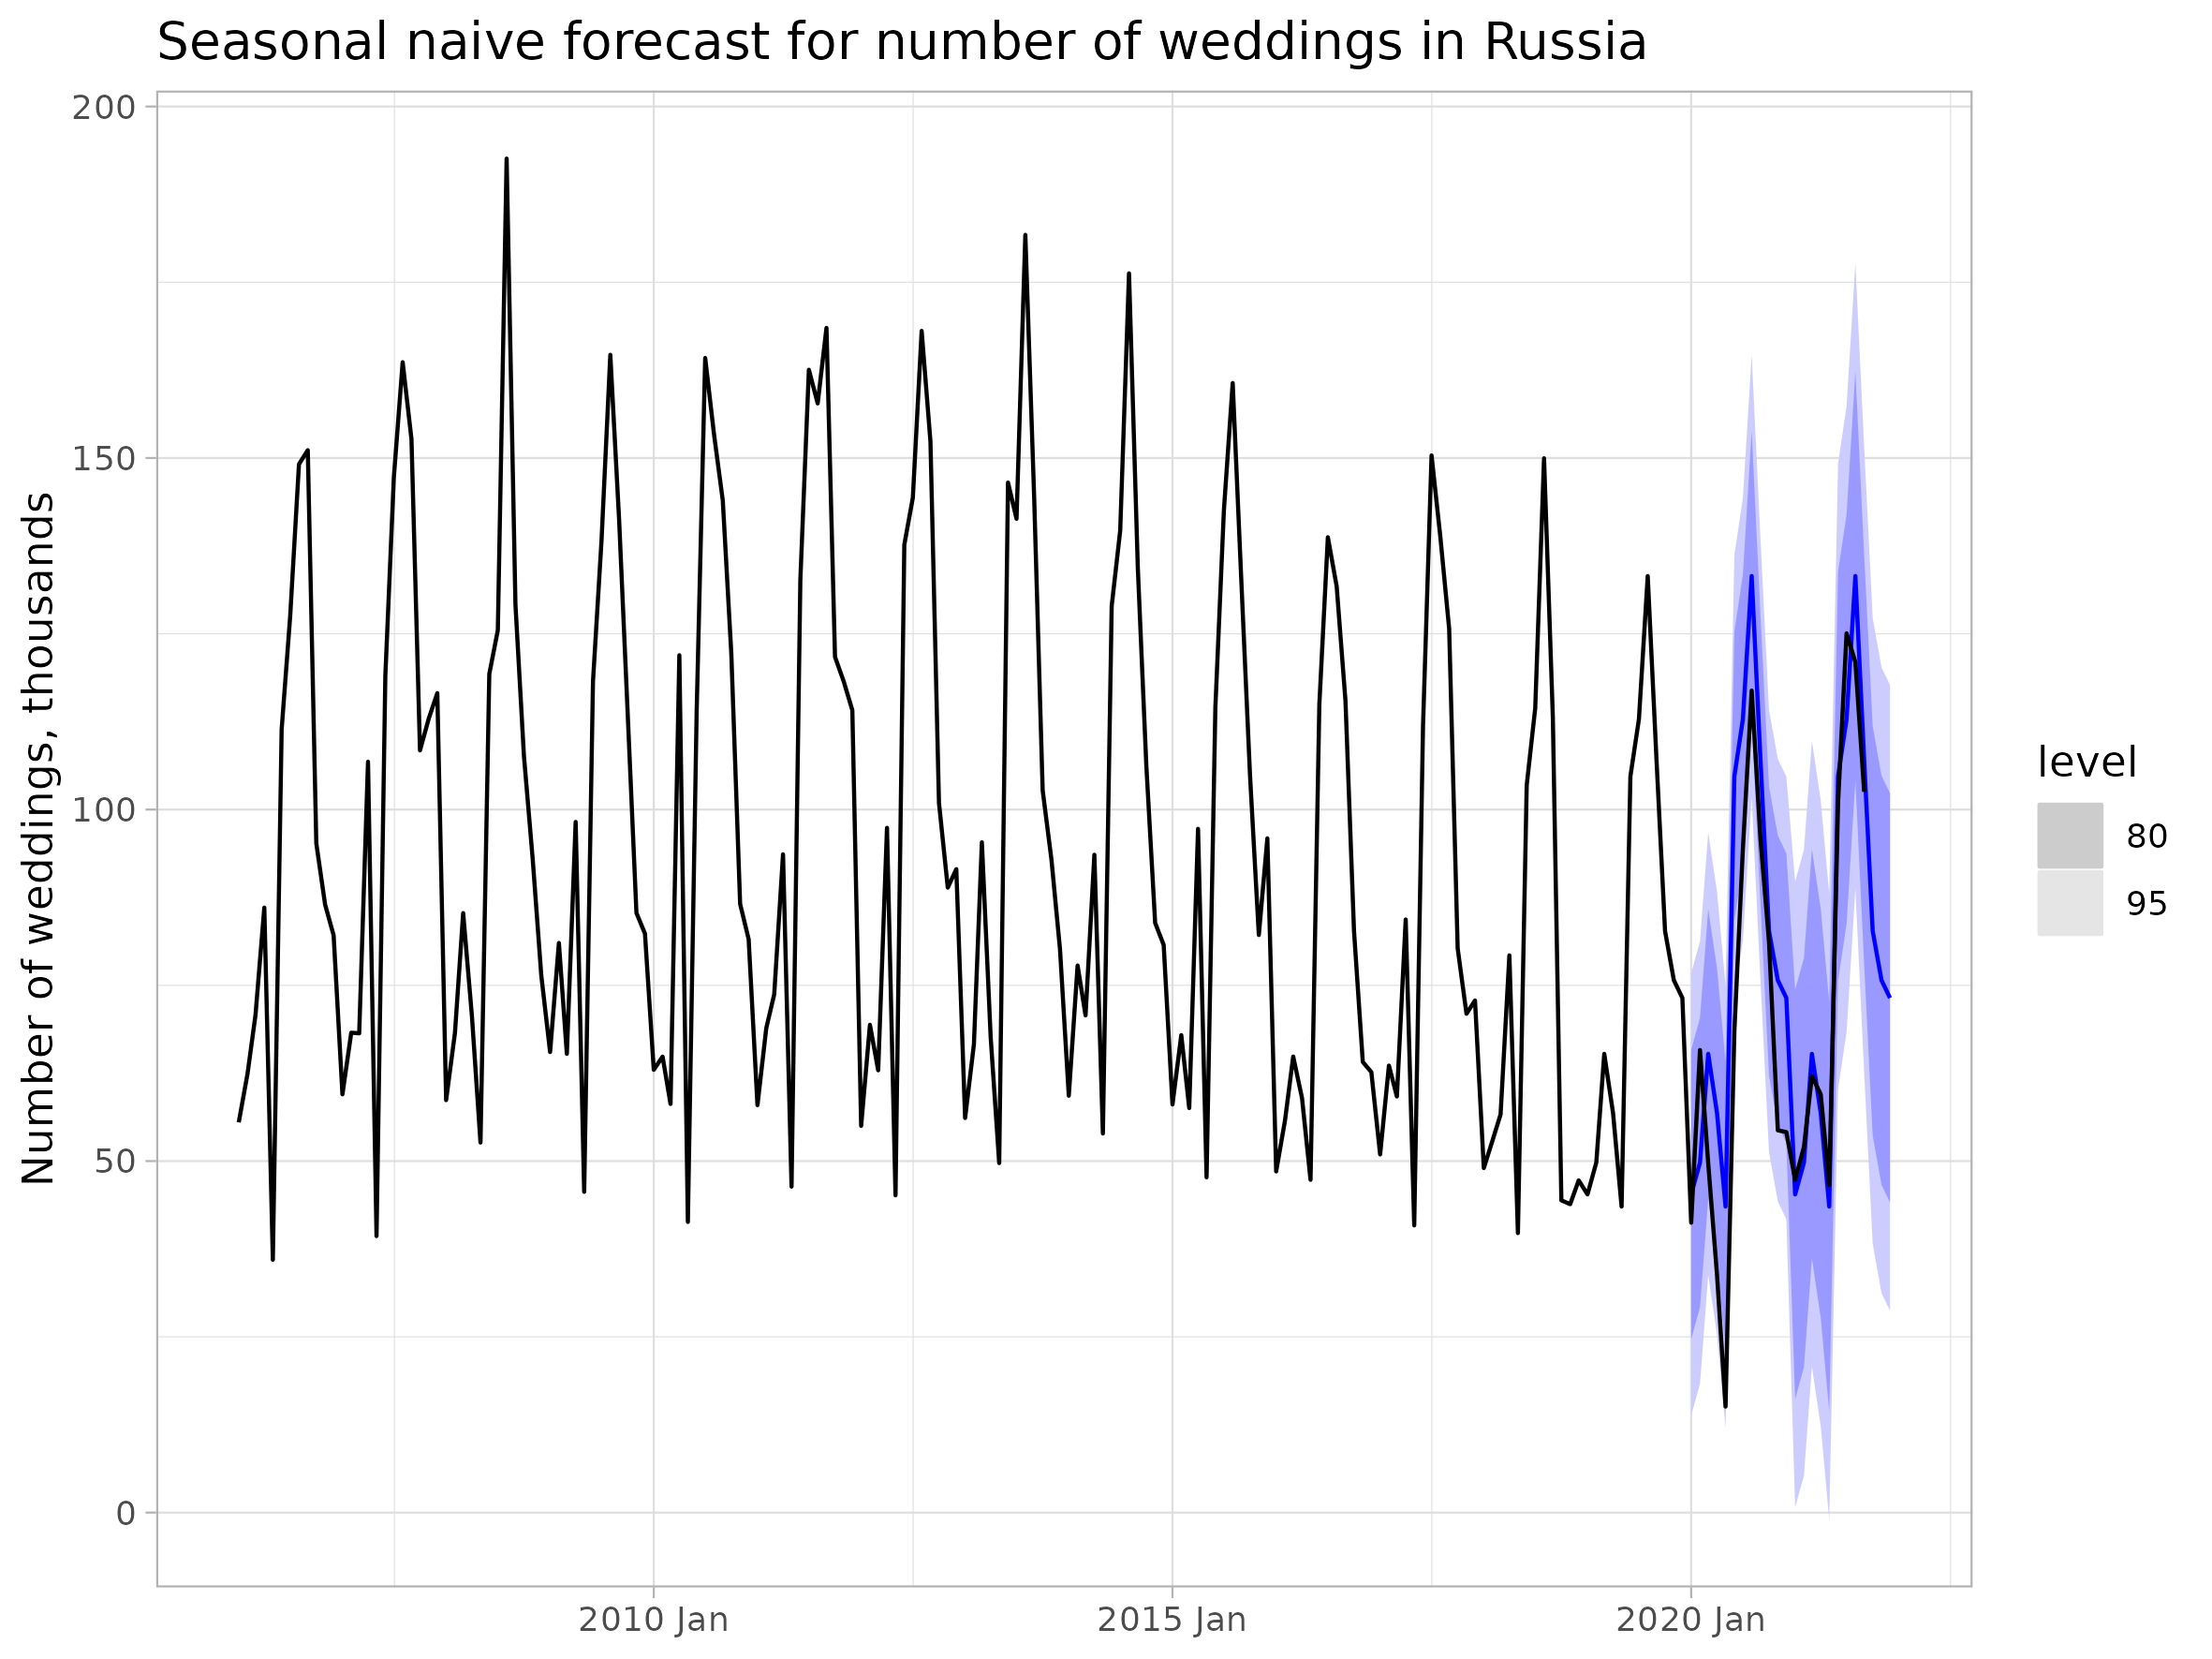
\includegraphics[width=\textwidth]{pictures/om_ts_01-017.png}
	
\end{frame}


\begin{frame}{Tasks for multiple series}
	
	\begin{itemize}[<+->]
		\item Use additional series when studying the target series
		\item Understand if series are related
		\item Measure cause and effect relationships
		\item Classify the new series into one of the existing classes
		\item Understand which series are close to each other
		\item Cluster series into an unknown set of clusters
		\item \ldots
	\end{itemize}
	
\end{frame}

\begin{frame}{Measuring series proximity}
	
	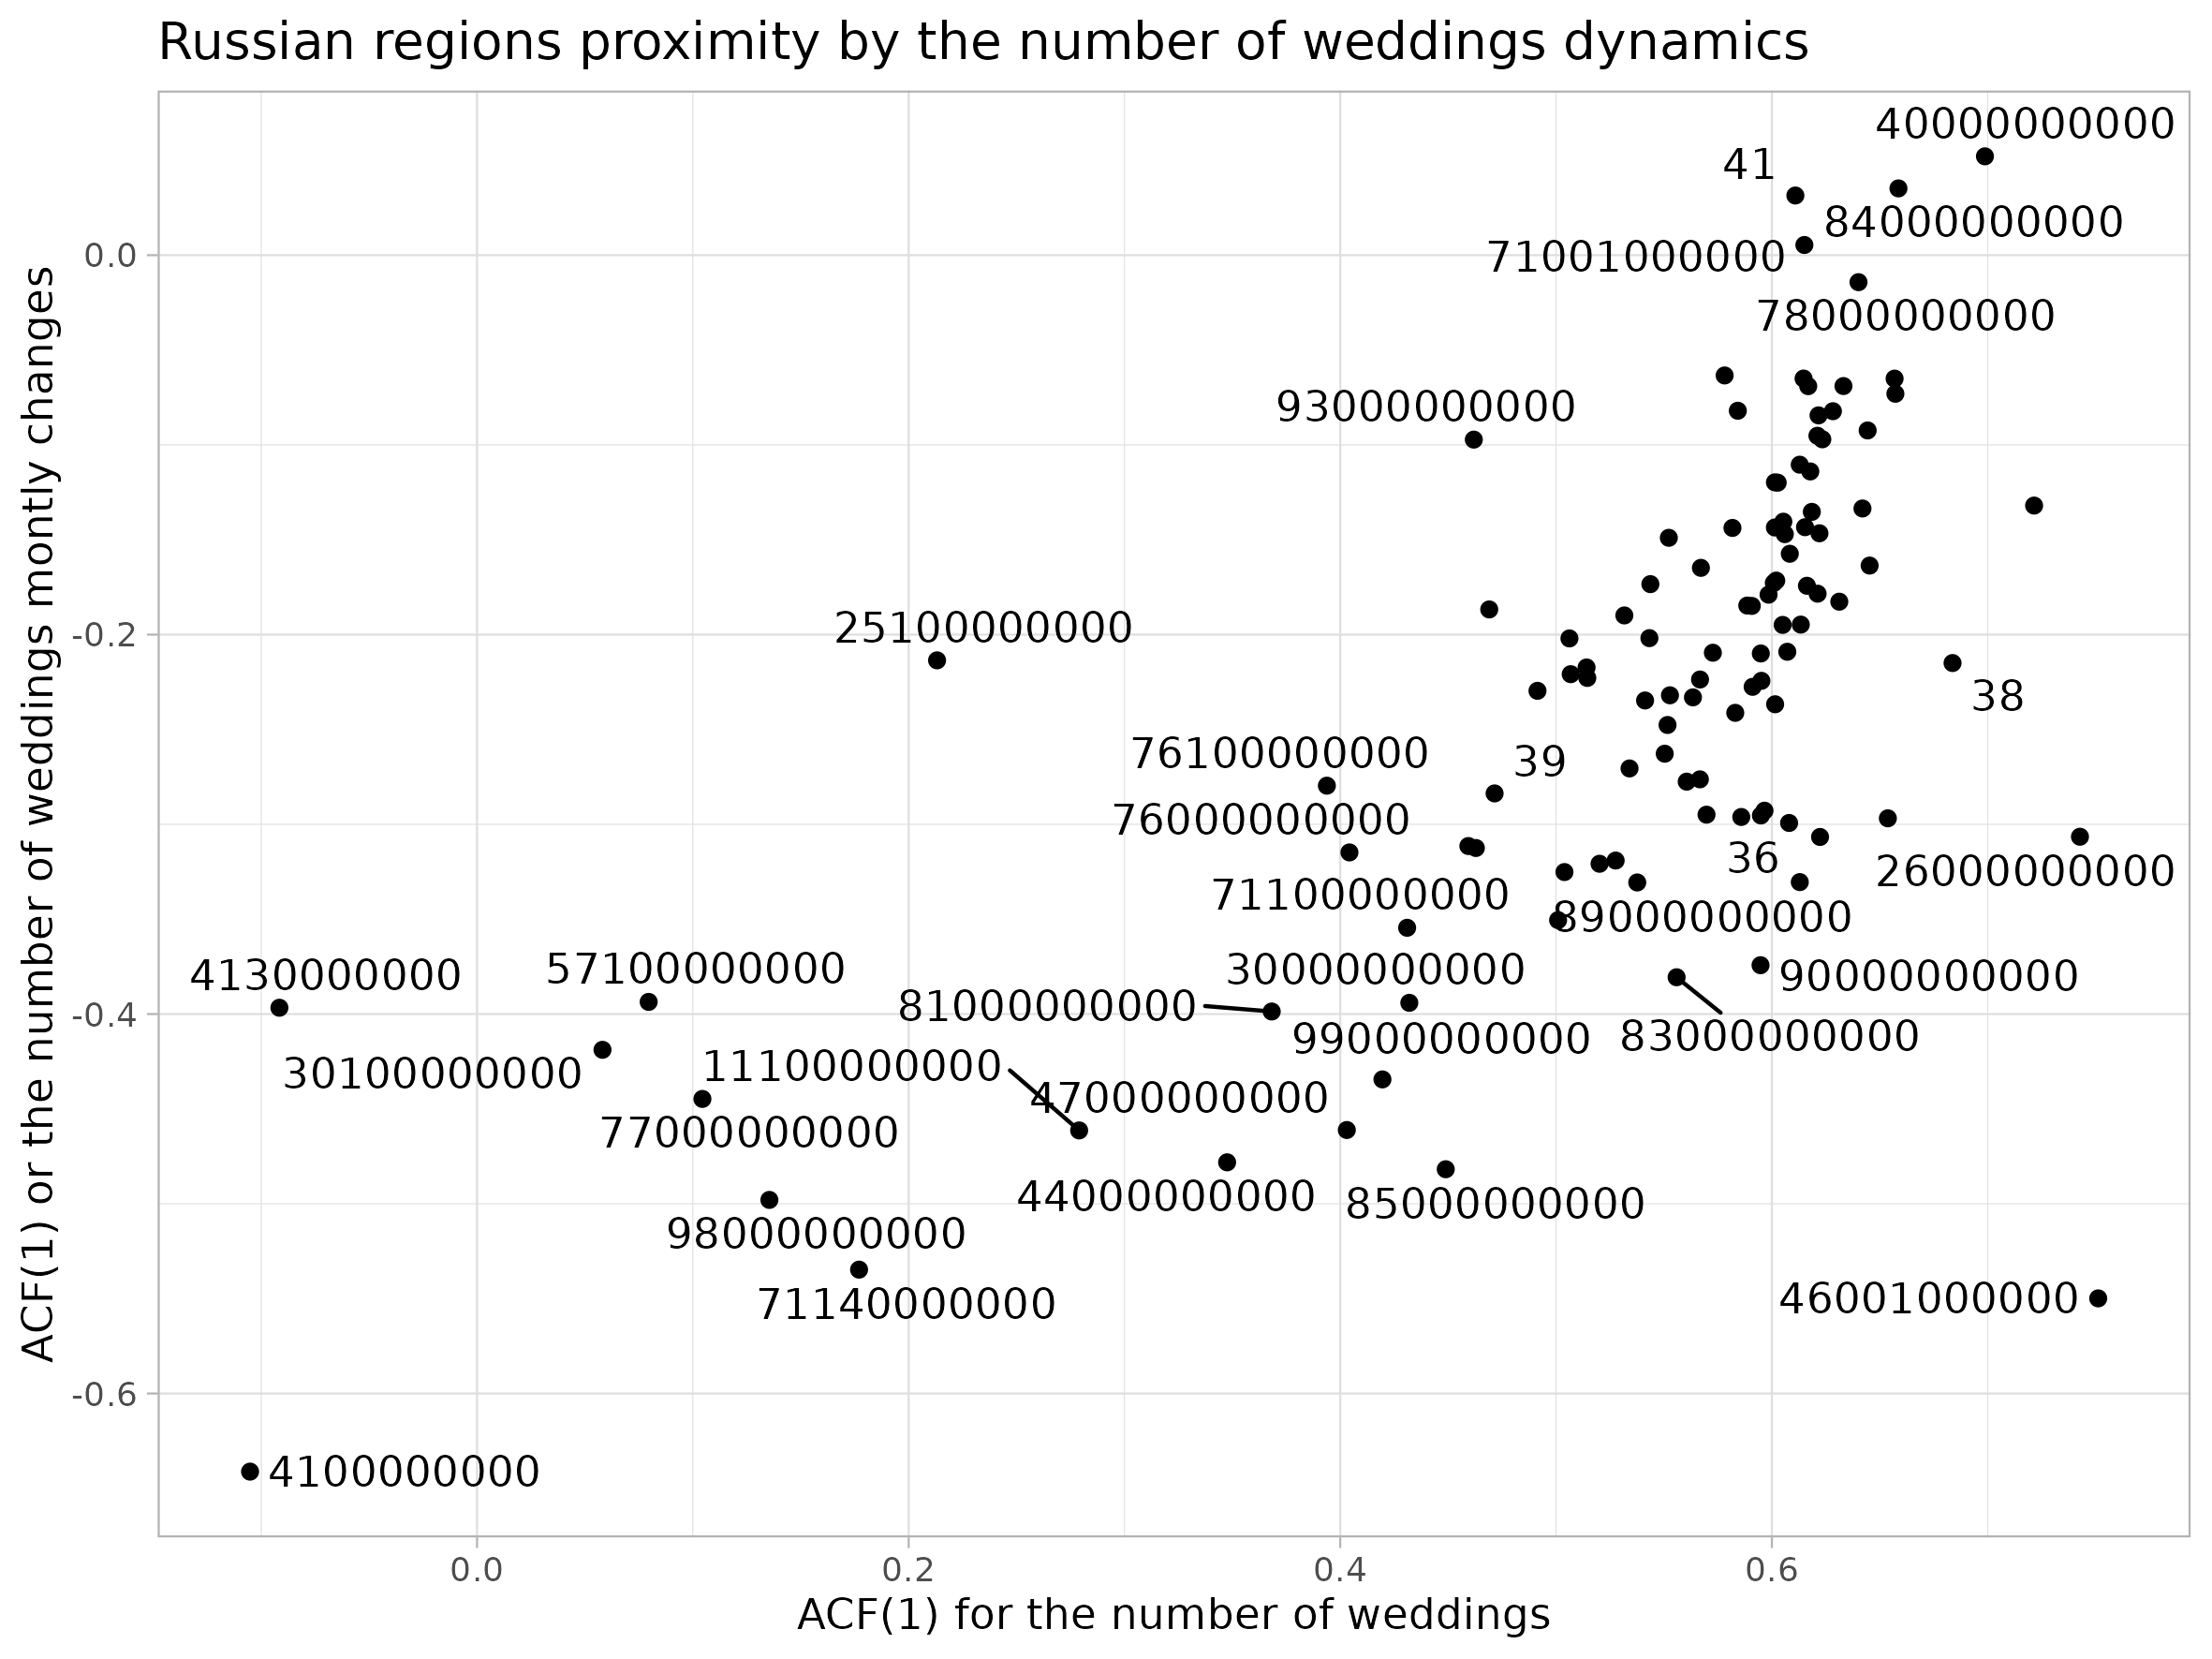
\includegraphics[width=\textwidth]{pictures/om_ts_01-025.png}
	
	
\end{frame}



\begin{frame}{Models and algorithms}
	
	\begin{block}{Models}
		\begin{itemize}[<+->]
			\item Explicit assumptions about the values $y_1$, $y_2$, \ldots, $y_T$
			\item Estimation method: maximum likelihood, Bayesian approach
			\item Point and interval forecasts, hypothesis testing
		\end{itemize}
	\end{block}
	
	ETS, ARIMA, ORBIT, PROPHET, \ldots
	
\end{frame}

\begin{frame}{Models and algorithms}
	
	\begin{block}{Algorithms}
		\begin{itemize}[<+->]
			\item Fuzzy assumptions about the values $y_1$, $y_2$, \ldots, $y_T$
			\item A special instruction for actions
			\item Point estimates without confidence intervals
		\end{itemize}
	\end{block}
	
	STL, gradient boosting, random forest, \ldots
	
\end{frame}

\begin{frame}{Course Focus}
	
	Forecasting one-dimensional series using models
	
\end{frame}

% !TEX root = ../om_ts_01.tex

\begin{frame} % frame name
	
	\videotitle{Series Components}
	
\end{frame}



\begin{frame}{Series Components: Plan}
	\begin{itemize}[<+->]
		\item Trend, cyclicity and seasonality
		\item Additive and multiplicative decomposition
		\item A formal definition?
	\end{itemize}
	
\end{frame}


\begin{frame}{Looking for components}
	
	Additive series decomposition:
	\[
	y_t = trend_t + seas_t + remainder_t
	\]
	
	\pause
	
	\alert{Trend} — smoothly changing component of the series
	
	\pause
	
	\alert{Seasonal component} — a component with a clear frequency and stable intensity
	
	\pause
	
	\alert{Random component} (remainder) — everything else
	
\end{frame}

\begin{frame}{Trend, seasonality and residual}
	
	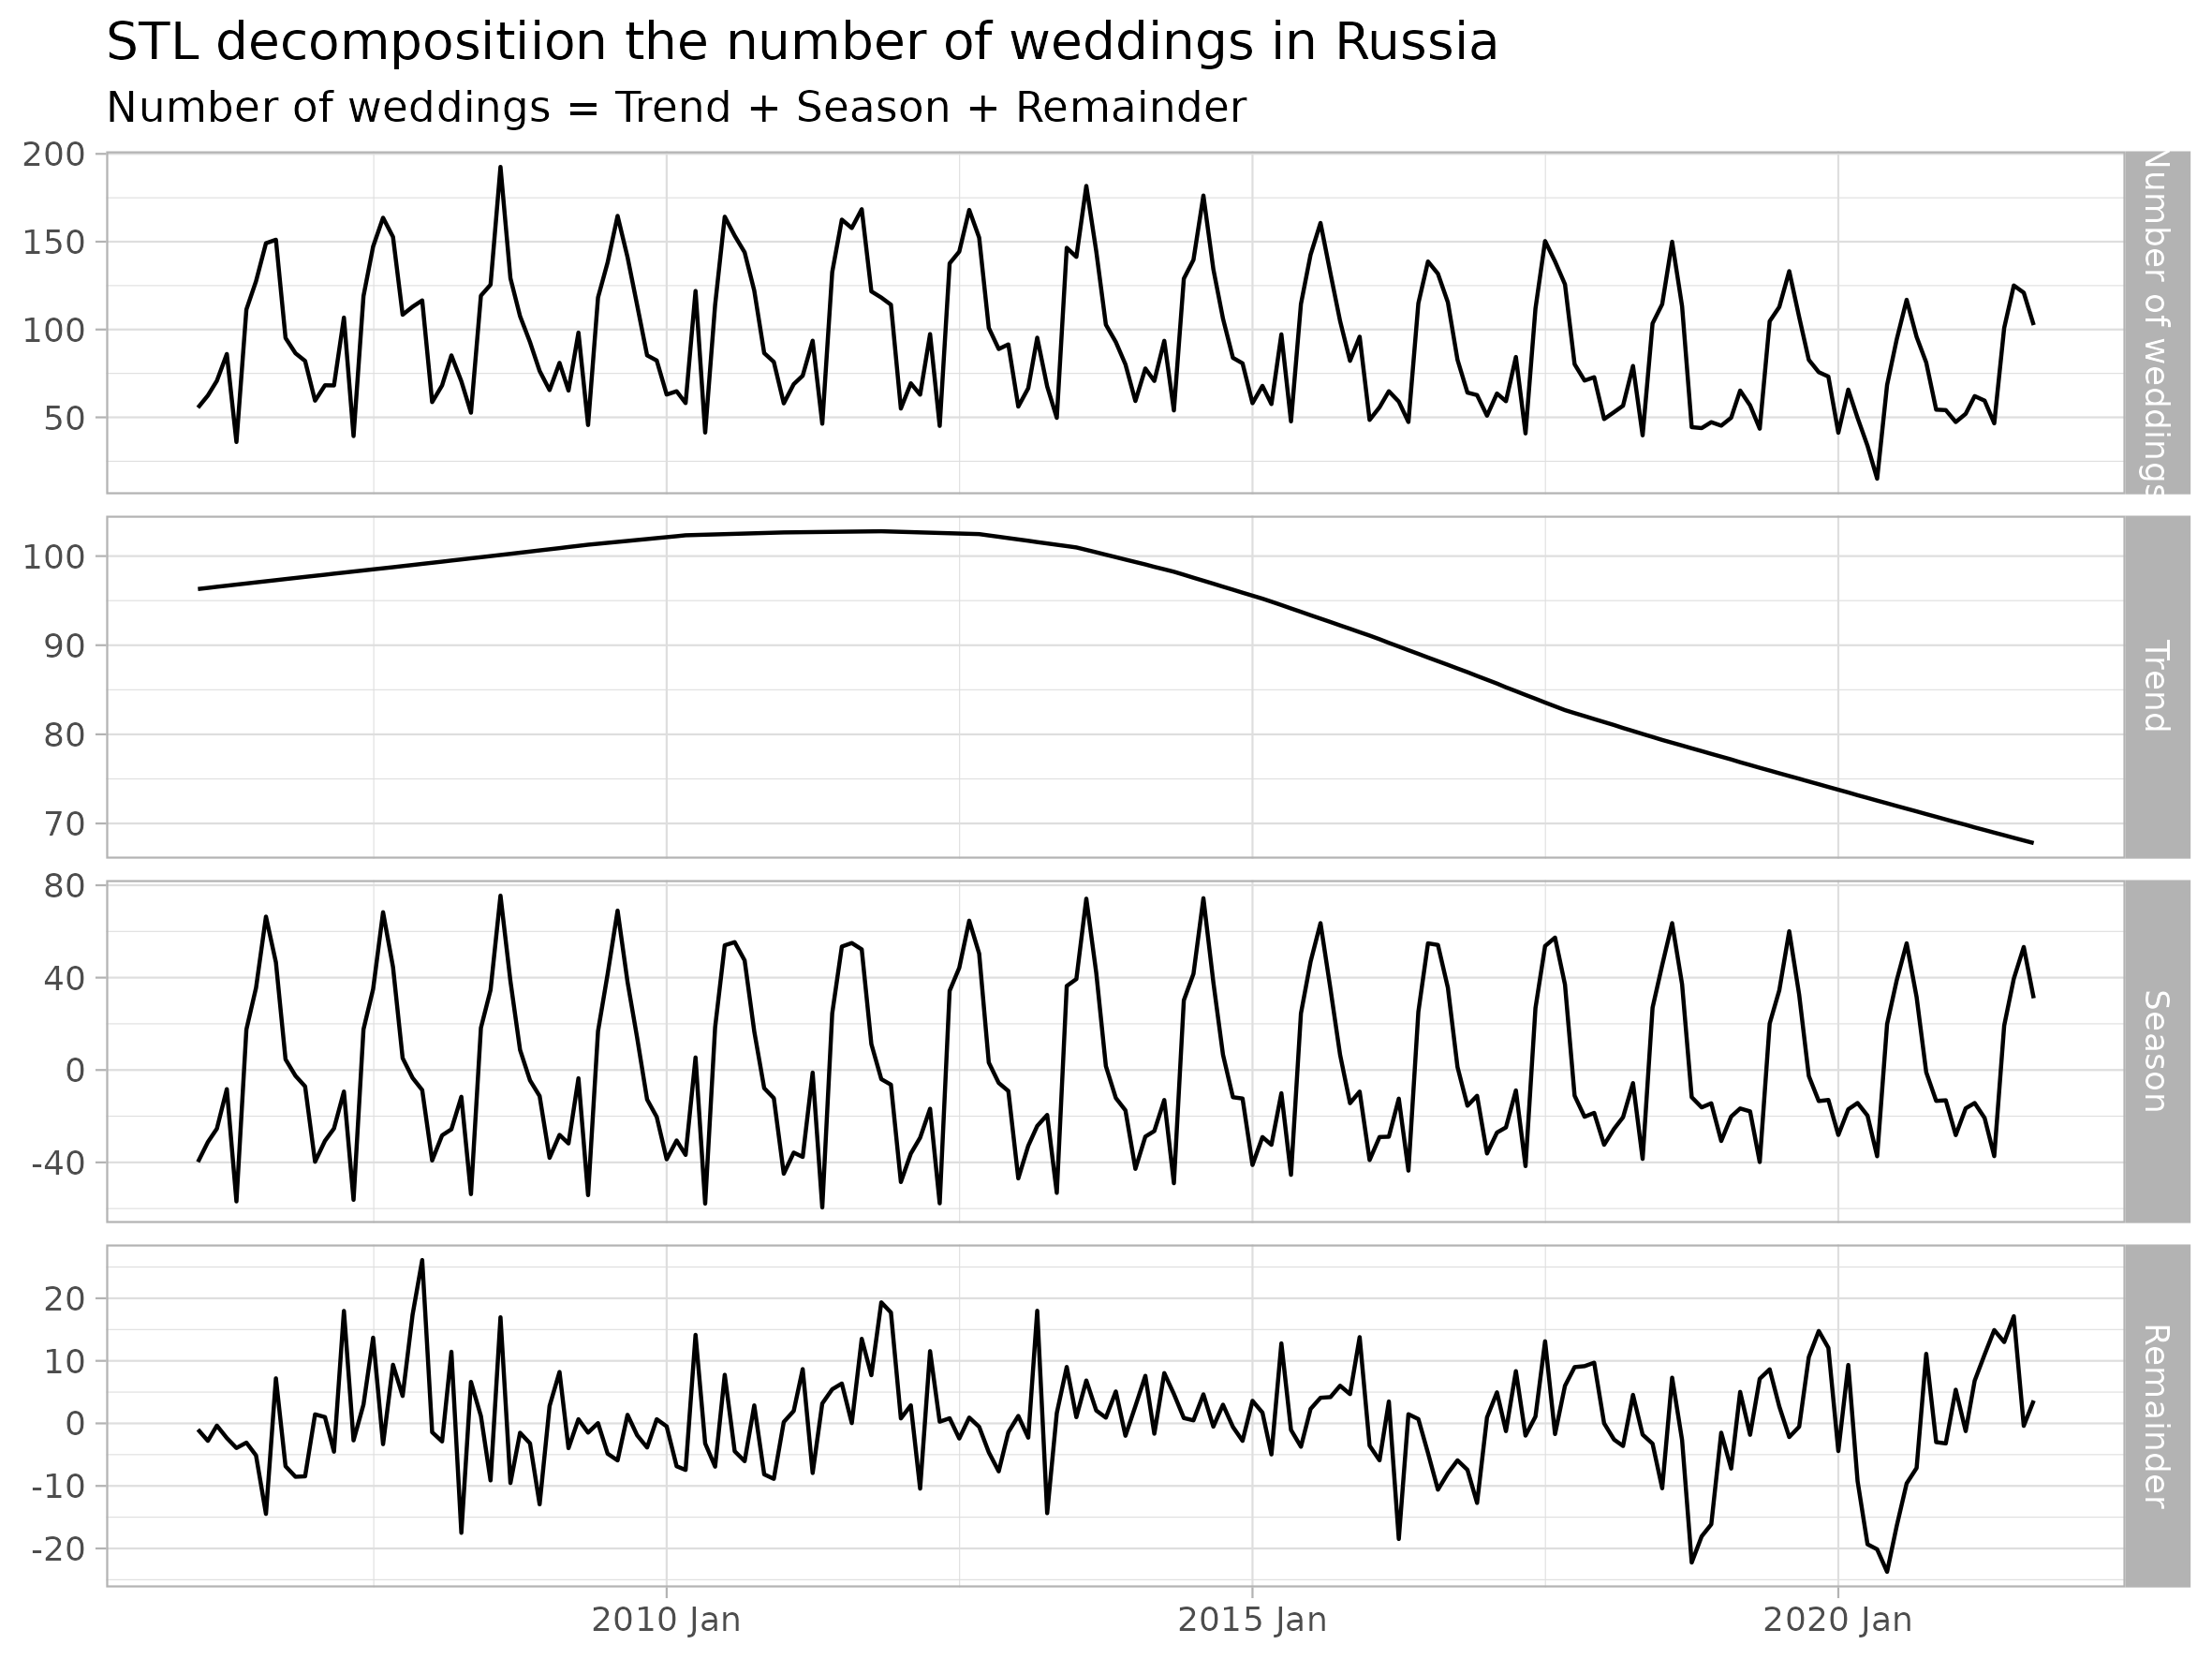
\includegraphics[width=\textwidth]{pictures/om_ts_01-041.png}
	
\end{frame}

\begin{frame}{Strict definition?}
	


	There will be no single strict definition for the components!
	
	\pause
	Some models and algorithms formally \alert{define} these components
	
\end{frame}

\begin{frame}{Cyclical component}
	
	Sometimes the series can be decomposed further
	\[
	y_t = trend_t + cycle_t + seas_t + remainder_t
	\]
	
	\pause
	\alert{Cyclical component} — component with floating frequency and unstable intensity
	
	
	\pause
	\alert{Trend} (in the narrow sense) — a smoothly changing monotonous component of a series
	
\end{frame}


\begin{frame}{Additive and multiplicative decomposition}
	
	
	\alert{Additive} series decomposition:
	\[
	y_t = trend_t + seas_t + remainder_t
	\]
	
	\pause
	\alert{Multiplicative} series decomposition:
	\[
	y_t = trend_t \cdot seas_t \cdot remainder_t
	\]
	
	\pause
	Let's transform one into another:
	\[
	\ln y_t = \ln trend_t + \ln seas_t + \ln remainder_t
	\]
\end{frame}


\begin{frame}{Box-Cox Transformation}
	
	
	For $y_t$, whose fluctuations  increases with $y_t$, \alert{it's reasonable to try} the logarithm
	or the Box-Cox transformation.
	
	\pause
	Logarithm: $y_t \to \ln y_t$
	
	Box-Cox transformation: $y_t \to bc_{\lambda}(y_t)$
	
	\pause
	
	(\alert{Generalized}) Box-Cox transformation:
	\begin{equation*}
		bc_{\lambda}(y_t) =
		\begin{cases} \ln y_t, \text{ if } \lambda = 0, \\
			\operatorname{sign} (y_t) (\abs{y_t}^{\lambda} - 1)/\lambda, \text { if } \lambda \neq 0
		\end{cases}
	\end{equation*}
	
	
	\pause
	
	How to \alert{select} the parameter $\lambda$?
	
	\pause
	
	
	\begin{itemize}[<+->]
		\item Some models contain it inside  and \alert{estimate} $\lambda$ within themselves
		\item You can choose $\lambda$ by yourself to \alert{stabilize the amplitude} of oscillations of the series
		
	\end{itemize}
	
	
\end{frame}






\begin{frame}{What to choose?}
	
	The formal definition of \alert{depends on the model}
	
	\pause
	\alert{STL algorithm}: one decomposition $y_t = trend_t + seas_t + remainder_t$
	
	\pause
	\alert{ETS(AAA)}: different decomposition $y_t = trend_t + seas_t + remainder_t$
	
	
	\pause
	It is important to understand the \alert{purpose of constructing} the decomposition
	
\end{frame}

\begin{frame}{Why decompose?}
	
	\begin{itemize}[<+->]
		\item Interesting \alert{by itself}
		\item For \alert{predicting} a series using component prediction
		\item To get \alert{characteristics of the series}
	\end{itemize}
	
	\pause
	Why characteristics?
	
	\begin{itemize}[<+->]
		\item To classify the new series into one of the given classes
		\item To identify unknown clusters in series
	\end{itemize}
	
\end{frame}


\begin{frame}{Series Components: Summary}
	\begin{itemize}[<+->]
		\item Trend \alert{smoothly changes} and includes a cyclical component
		\item The seasonal component has \alert{clear periodicity} and \alert{stable amplitude}
		\item The exact formalization of the components \alert{depends on the model}
	\end{itemize}
	
\end{frame}

\begin{frame} % frame name
	
	\videotitle{Naive Models}
	
\end{frame}



\begin{frame}{Naive Models: Plan}
	\begin{itemize}[<+->]
		\item White noise
		\item Independent observations
		\item Random walk
	\end{itemize}
	
\end{frame}

\begin{frame}{White noise}
	
	\begin{block}{White noise}
		Time series $u_t$ is white noise if:
		\begin{itemize}
			\item $\E(u_t) = 0$;
			\item $\Var(u_t) = \sigma^2$;
			\item $\Cov(u_s, u_t) = 0$ for $s\neq t$
		\end{itemize}
	\end{block}
	
	\pause
	\begin{itemize}[<+->]
		\item An integral part of all models; most often, white noise is not modelled explicitly
		\item Often \alert{independence} and \alert{normality} are  assumed 

		
		ARCH, GARCH volatility models are based on the fact that $u_t$ and $u_s$ can be dependent!
	\end{itemize}
	
\end{frame}


\begin{frame}{Independent observations}
	
	\begin{block}{Model}
		\[
		y_t = \mu + u_t,
		\]
		where $u_t$ is white noise, $u_t \sim \dN(0;\sigma^2)$
	\end{block}
	\pause
	\alert{Estimators:}
	\[
	\hat \mu_{ML} = \bar y, \quad \hat\sigma^2_{ML} = \frac{\sum(y_i - \bar y)^2}{T}
	\]
	\pause
	\alert{Interval forecast} $h$ steps ahead:
	\[
	[\bar y - 1.96 \hat\sigma; \bar y + 1.96 \hat \sigma]
	\]
\end{frame}


\begin{frame}{Random Walk}
	
	\begin{block}{Naive model}
		\[
		y_t = y_{t-1} + u_t,
		\]
		where $u_t$ is white noise, $u_t \sim \dN(0;\sigma^2)$, starting $y_1$ is given
	\end{block}
	\pause
	Let's reformulate: $y_t - y_{t-1} = \Delta y_t = u_t$
	
	
	\pause
	\alert{Estimators:}
	\[
	\hat\sigma^2_{ML} = \frac{\sum(\Delta y_i - \overline {\Delta y})^2}{T - 1}
	\]
	\pause
	\alert{Interval forecast} $h$ \alert{steps} ahead:
	\[
	[y_T - 1.96 \hat \sigma \sqrt{h}; y_T + 1.96 \hat \sigma \sqrt{h}]
	\]
\end{frame}

\begin{frame}{First predictions!}
	
	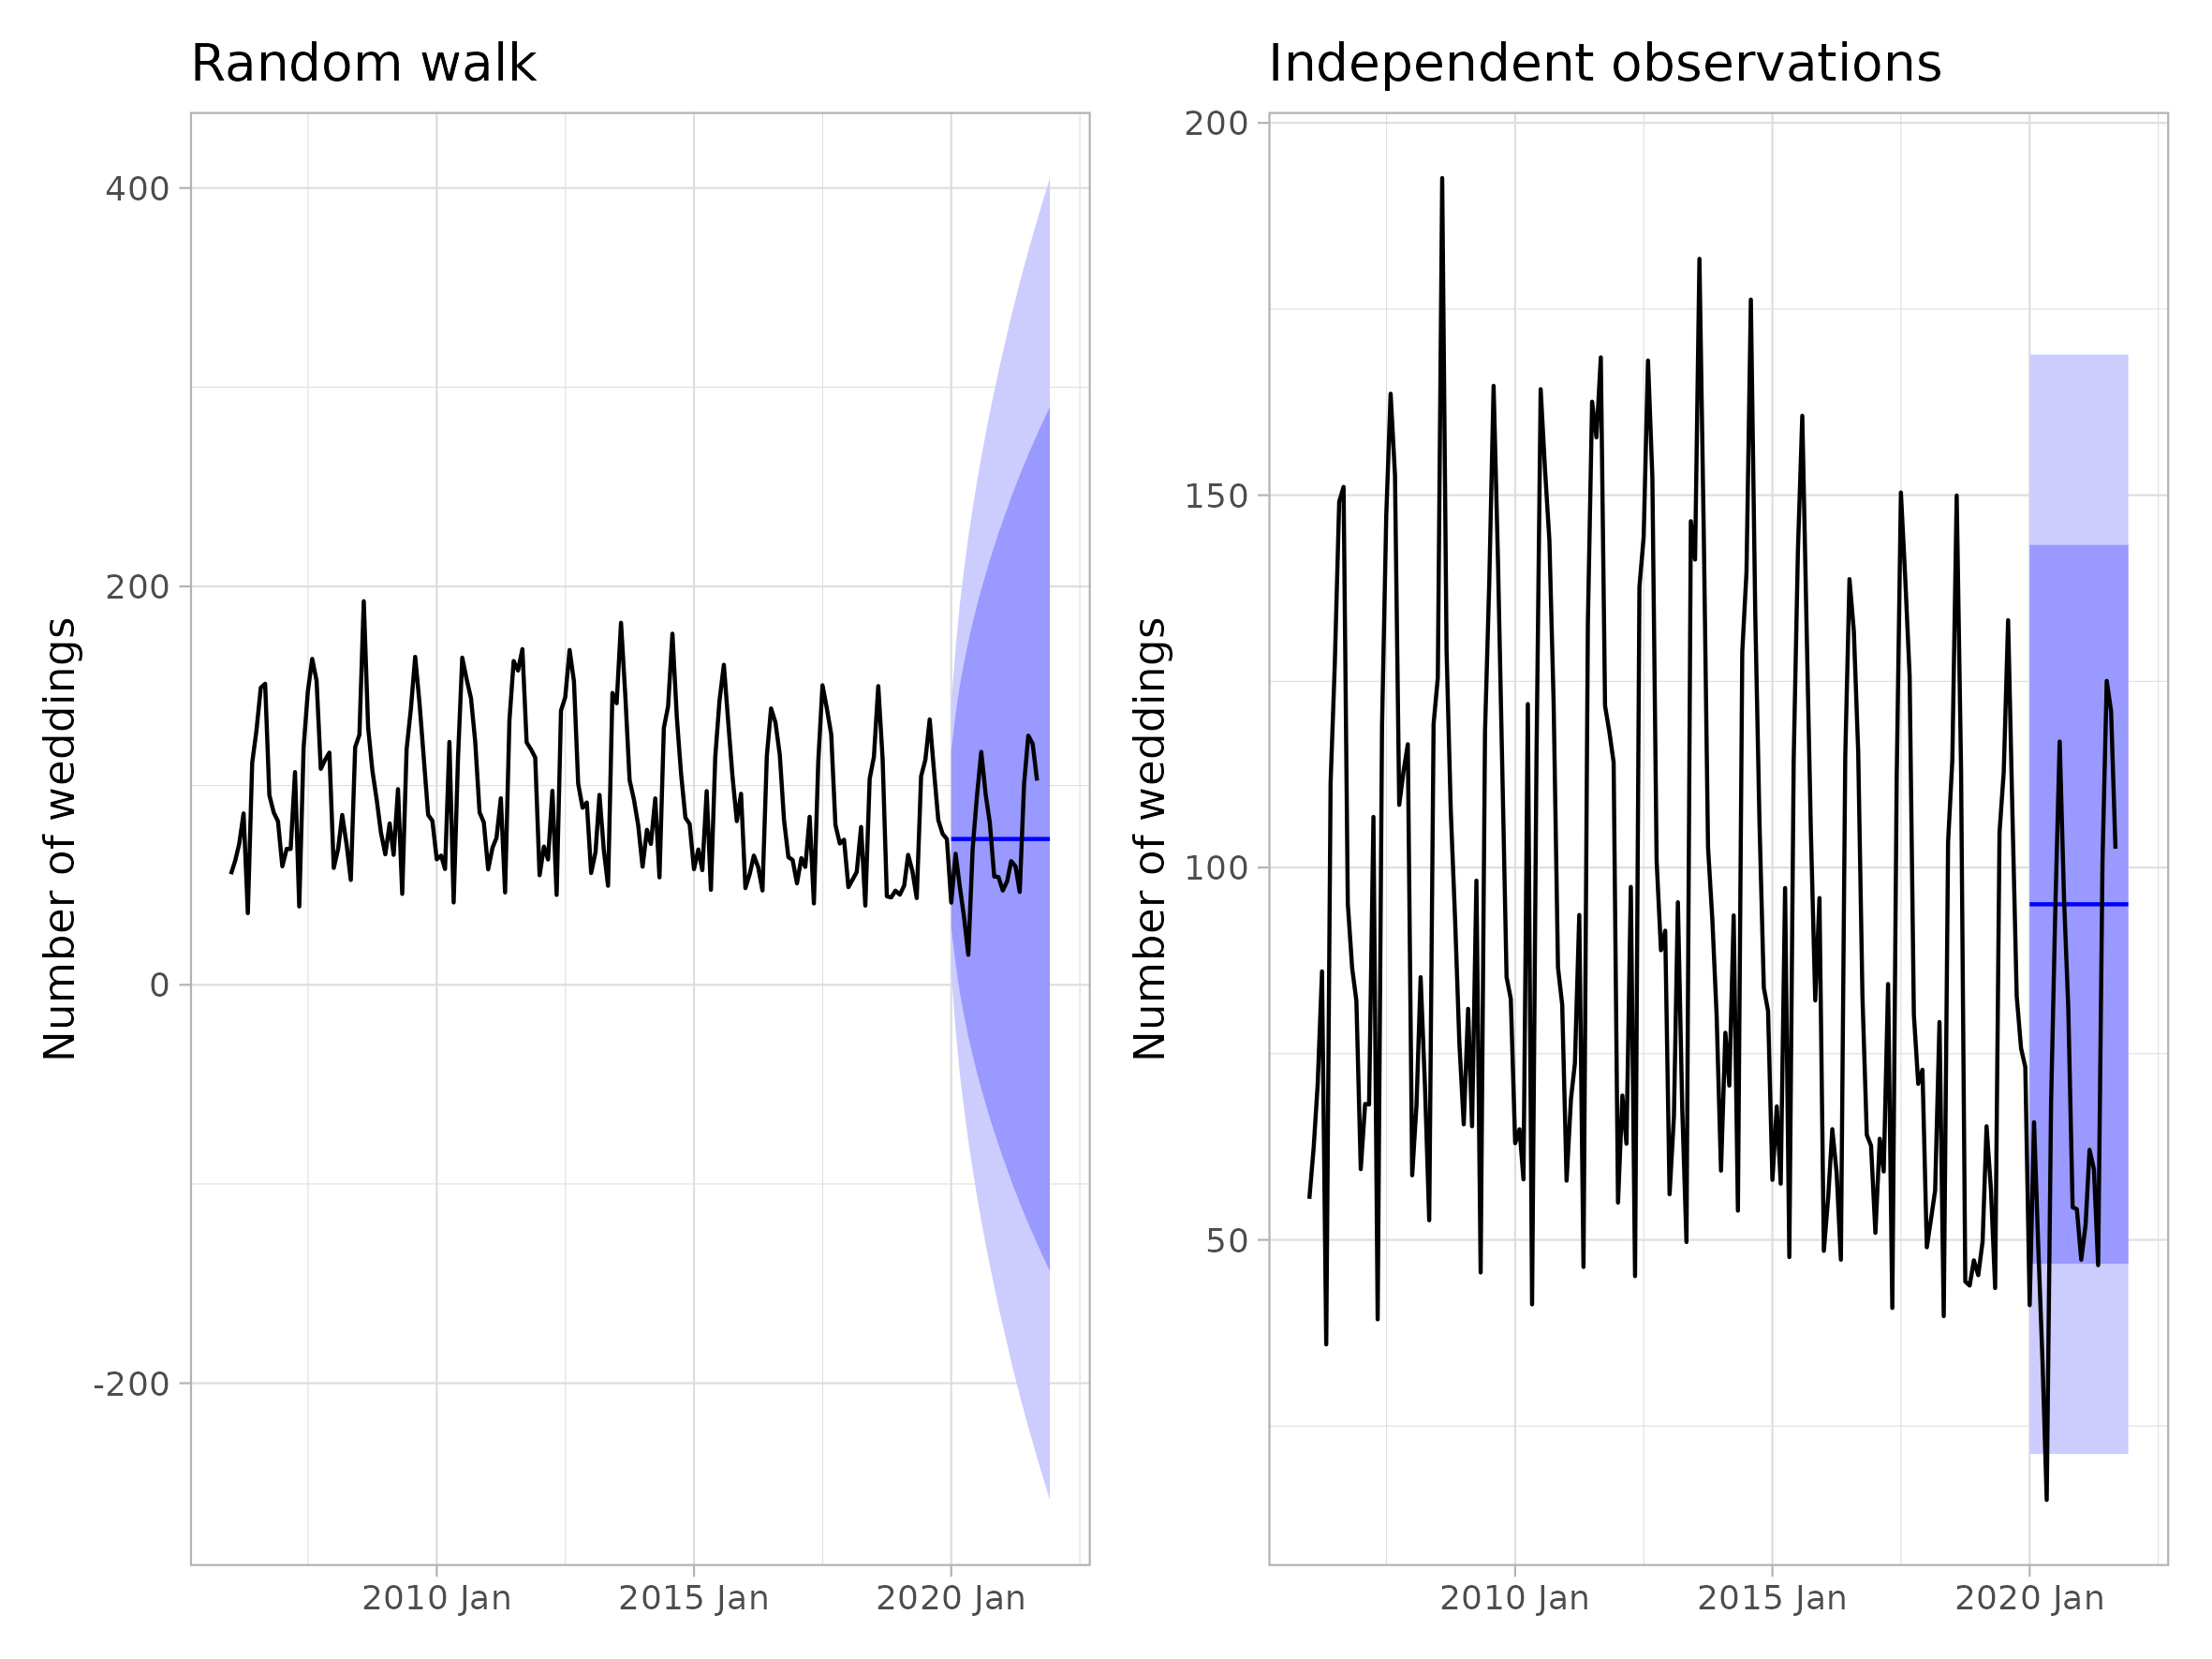
\includegraphics[width=\textwidth]{pictures/om_ts_01-157.png}
	
\end{frame}


\begin{frame}{Seasonal random walk}
	
	\begin{block}{Seasonal naive model}
		\[
		y_t = y_{t-12} + u_t,
		\]
		where $u_t$ is white noise, $u_t \sim \dN(0;\sigma^2)$, $y_1$, \ldots, $y_{11}$ are given
	\end{block}
	\pause
	Let's reformulate: $y_t - y_{t-12} = \Delta_{12} y_t = u_t$
	\pause
	
	\alert{Estimators:}
	\[
	\hat\sigma^2_{ML} = \frac{\sum(\Delta_{12} y_i - \overline {\Delta_{12} y})^2}{T - 12}
	\]
	\pause
	\alert{Interval forecast} for $h$ \alert{steps} ahead:
	\[
	\left[y_{T-12+h\%12} - 1.96 \hat \sigma \sqrt{\left\lceil \frac{h}{12} \right\rceil}; y_{T-12+h\%12} + 1.96 \hat \sigma \sqrt{\left\lceil \frac{h}{12} \right\rceil}\right]
	\]
	
	where $\%$ - remainder from the division, $\lceil x \rceil$ - ceiling function
 	
	
\end{frame}
	
	


\begin{frame}{Not bad already!}
	
	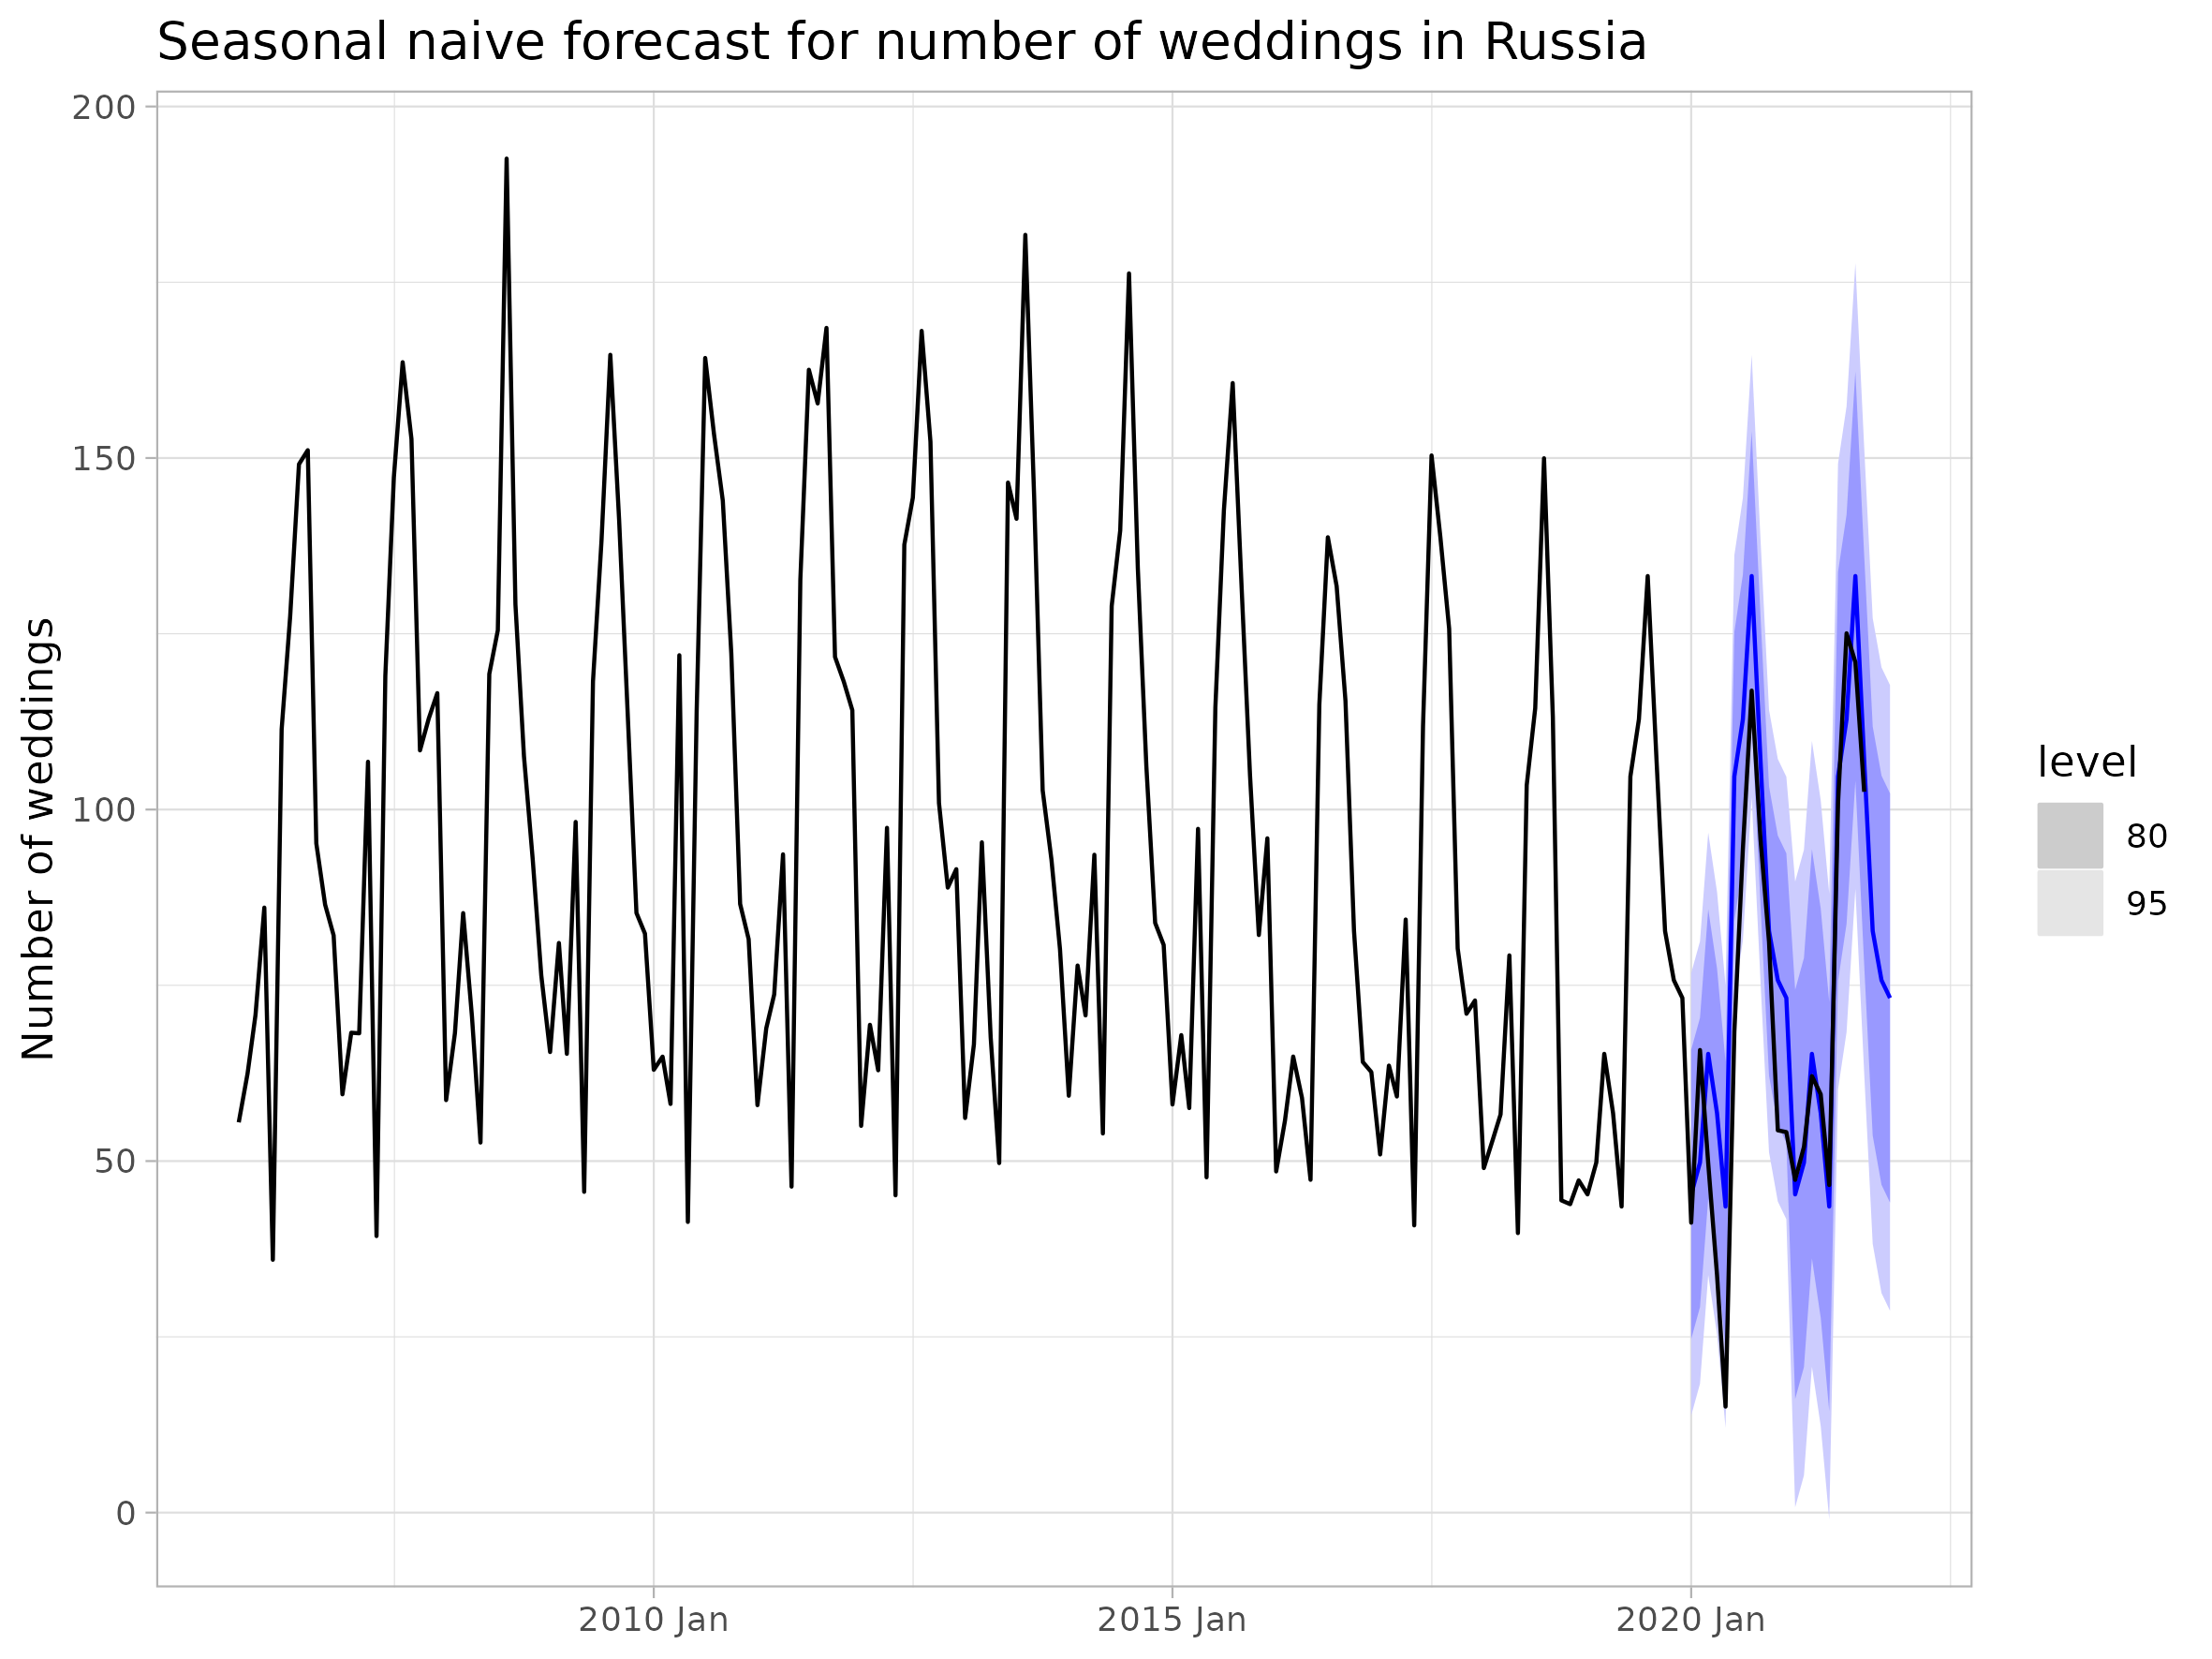
\includegraphics[width=\textwidth]{pictures/om_ts_01-162.png}
	
	
\end{frame}


\begin{frame}
	\frametitle{Why do we need naive models?}
	
	\begin{itemize}[<+->]
		\item \alert{Ideas} for complex model:
		
		the \alert{stationary series} models are similar to the independent observations model;
		
		\alert{non-stationary series} models are similar to a random walk
		
		\item \alert{Benchmark for comparison}:
		
		when evaluating a complex model, it is very important to have a base of comparison
		
		\item \alert{Averaging} with other models' forecasts:
		
		you can \alert{average forecasts} of a complex model and a naive seasonal one!
	\end{itemize}
	
	
\end{frame}

\begin{frame}{Naive Models: Summary}
	
	\begin{itemize}[<+->]
		\item White noise is what you don't want to simulate
		\item Independent observations and random walk
		\item Ideas, parts, and helpers for other models
		\item Base for comparison
	\end{itemize}
\end{frame}

% !TEX root = ../om_ts_01.tex

\begin{frame} % frame name
	
	\videotitle{STL algorithm}
	
\end{frame}



\begin{frame}{STL algorithm: Plan}
	\begin{itemize}[<+->]
		\item Local regression
		\item STL outer loop
		\item STL inner loop
		\item STL options
	\end{itemize}
	
\end{frame}


\begin{frame}{STL}
	
	\alert{STL} — Seasonal Trend decompositon with LOESS
	
	STL — seasonality and trend decomposition using LOESS
	
	\pause
	
	\alert{LOESS} — LOcal regrESSion
	
	LOESS — local linear regression
	
\end{frame}


\begin{frame}{STL as a black box}
	
	\alert{Input:}
	
	Row $Y_t$
	
	Algorithm parameters $n_p$, $n_i$, $n_o$, $n_l$, $n_s$, $n_t$
	
	\pause
	\alert{Output:}
	
	Decomposition $Y_t = T_t + S_t + R_t$
	
	\pause
	
	Black box set up
	
\end{frame}


\begin{frame}{STL: result}
	
	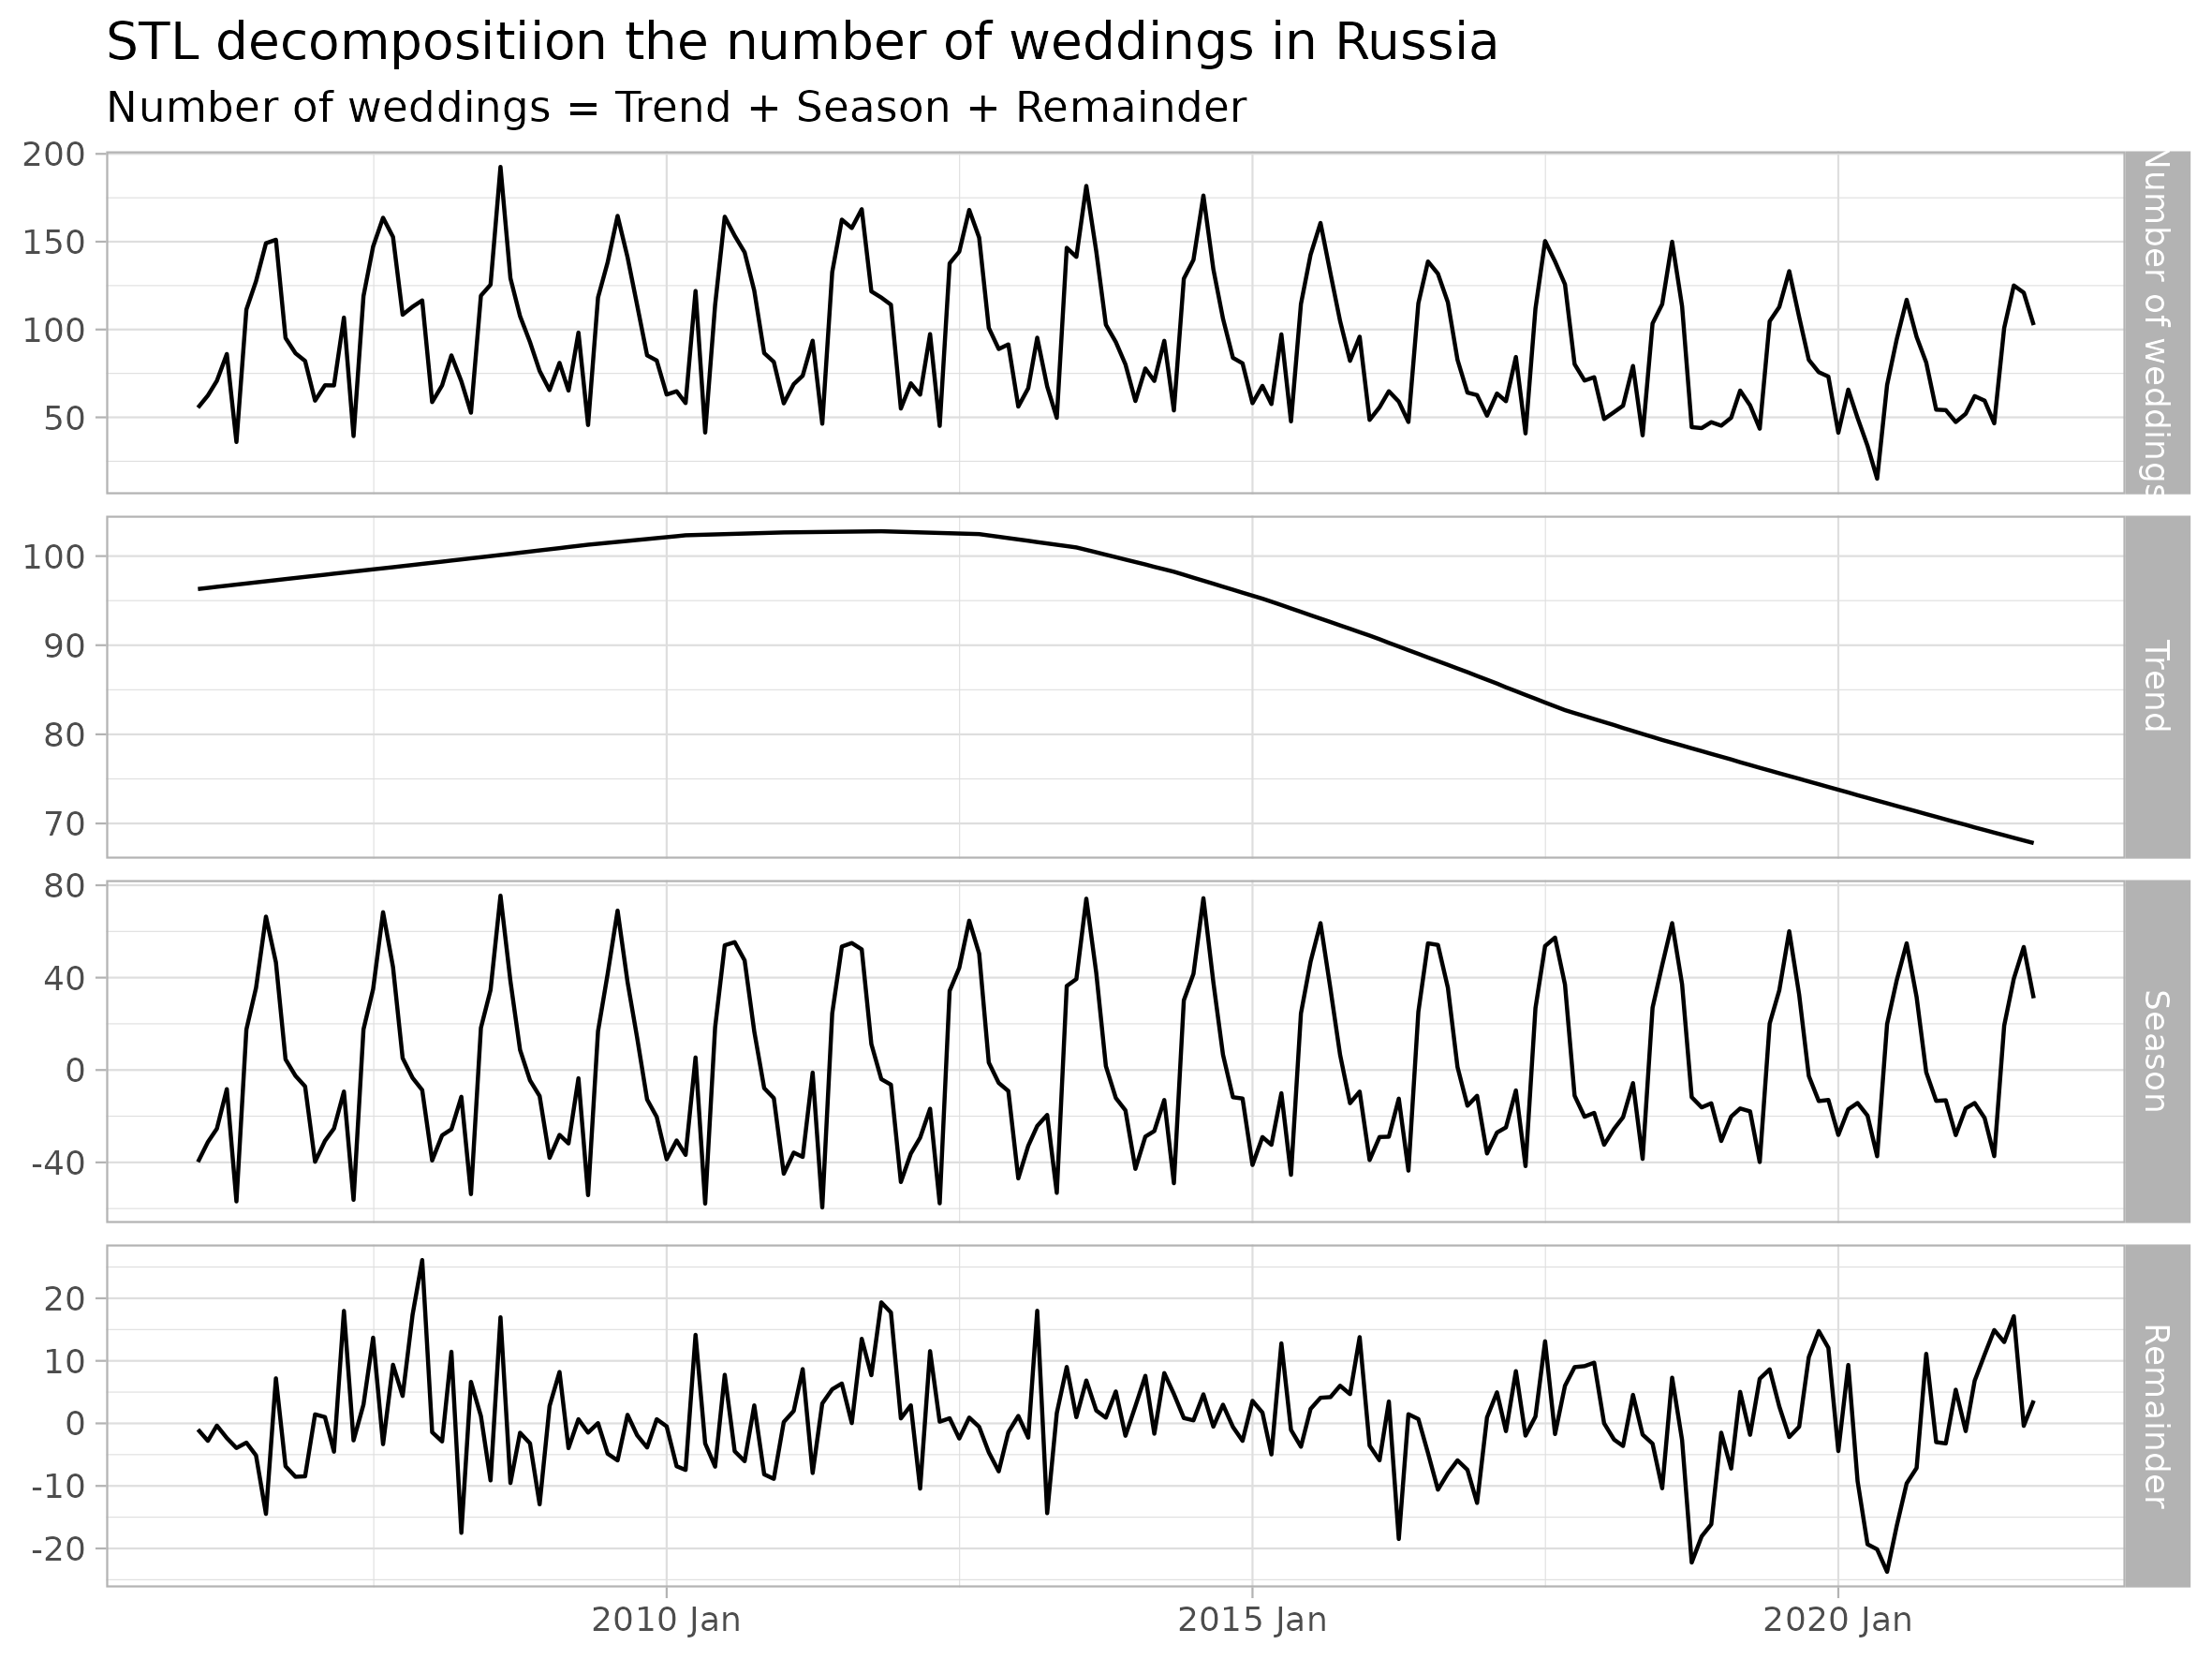
\includegraphics[width=\textwidth]{pictures/om_ts_01-074.png}
	
	
\end{frame}

\begin{frame}{LOESS}
	
	\begin{itemize}
		\item We want to build a forecast for the point $x$
		\item Find \alert{local estimates} $\hat\beta_1(x)$, $\hat\beta_2(x)$
		\[
		\min \sum_i \alert{K_h(x_i - x)} (y_i - \hat\beta_1 - \hat\beta_2 x_i)^2
		\]
		\item Predicting:
		\[
		\hat y = \hat\beta_1(x) + \hat\beta_2(x) x.
		\]
	\end{itemize}
	
	\pause
	\alert{Kernel function}
	\begin{itemize}
		\item The function $K_h(x_i - x)$ decreases with increasing distance $|x_i - x|$;
		\item The $h$ parameter controls the width of the smoothing window
	\end{itemize}
	
	\pause
	For example, $h$ is the number of points $x_i$ next to $x$ that we take into account
	
\end{frame}

\begin{frame}{Nuances of local regression}
	
	\begin{itemize}
		\item Select \alert{degrees of the polynomial}
		\[
		\min \sum_i \alert{K_h(x_i - x)} (y_i - \hat\beta_1 - \hat\beta_2 x_i - \hat\beta_3 x_i^2)^2
		\]
		\item Select \alert{kernel} function
		\[
		K_h(d) = \frac{1}{\sqrt{2\pi}h} \exp(- d^2/2h^2)
		\]
		\item Select \alert{window width} $h$
		
	\end{itemize}
	
\end{frame}

\begin{frame}{STL algorithm}
	
	Purpose: decomposition of $Y_t = T_t + S_t + R_t$
	
	The algorithm contains two loops: \alert{outer} and \alert{inner} loop
	
	\begin{enumerate}[<+->]
		
		\item Initialize $T_t = 0$, $R_t = 0$
		
		\alert{Outer} loop:
		
		\item Calculate the weight of each observation, $\rho_t$:
		
		on the first pass, $\rho_t = 1$ for each observation;
		
		on subsequent passes, $\rho_t$ depends negatively on the new value of $R_t$
		
		\item Update the current decomposition $Y_t = T_t + S_t + R_t$ taking into account new weights $\rho_t$
	\end{enumerate}
	
\end{frame}



\begin{frame}{STL: inner loop}
	
	Goal: update the decomposition $Y_t = T_t + S_t + R_t$.
	
	\begin{enumerate}[<+->]
		
		\item[1.] Remove the previously calculated trend from the series:
		\[
		Y_t^{det} = Y_t - T_t.
		\]
		
		\item[2.] Divide the detrended series into 12 series (one for each season)
		
		\item[3.] Smooth each of the series individually with LOESS:
		\[
		C^{jan} = LOESS_{\rho}(Y^{det}_{jan}), C^{feb} = LOESS_{\rho}(Y^{det}_{feb}), \ldots
		\]
		
		\item[4.] Extract the low-frequency component (double moving average + LOESS):
		\[
		L_t = LOESS(MA(MA(C_t)))
		\]
	\end{enumerate}
	
	
\end{frame}



\begin{frame}{STL: inner loop}
	
	
	\begin{enumerate}		
		
		\item[1-3.] Remove the previously calculated trend from the series, break it down into 12 series and
		smooth each of them with LOESS.
		
		\item[4.] Extract the low-frequency component $L_t$.
		
		
		
	\end{enumerate}
	
	
	\begin{enumerate}[<+->]
		

		\item[5.] Get \alert{new} seasonal component  by removing the low-frequency component:
		\[
		S_t^{new} = C_t - L_t
		\]
		\item[6.] Get new trend component by removing  new seasonal component from the original series and smoothing with LOESS:
		\[
		T_t^{new} = LOESS_{\rho}(Y_t - S_t^{new})
		\]
		
	\end{enumerate}
	
	
\end{frame}




\begin{frame}{STL parameters}
	
	\begin{itemize}[<+->]
		\item $n_p$ — periodicity of seasonality, for example, $n_p=12$
		\item $n_o$ is the number of iterations of the outer loop:
		
		the larger the number $n_o$, the weaker the impact of outliers;
		
		$n_o = 1$ is often sufficient
		
		\item $n_i$ — number of passes of the inner loop:
		
		$n_i = 2$ is often enough to achieve convergence.
	\end{itemize}
	
\end{frame}

\begin{frame}{STL smoothing parameters}
	
	\begin{itemize}[<+->]
		\item $n_l$ — low pass filter smoothing strength
		
		\item $n_s$ — seasonal contract smoothing strength
		\item $n_t$ — smoothing strength when highlighting a trend at the last step
		
		
		
		\alert{What to configure?}
		
		
	\end{itemize}
	
	\begin{enumerate}[<+->]
		\item Be sure to specify the periodicity $n_p$
		\item Maybe play around with $n_s$
	\end{enumerate}
	
\end{frame}

\begin{frame}{STL algorithm: Summary}
	\begin{itemize}[<+->]
		\item LOESS — local regression
		\item STL is a well-proven algorithm without an underlying model
		\item If you wish, you can play around with the smoothing parameters
	\end{itemize}
	
\end{frame}




% !TEX root = ../om_ts_01.tex

\begin{frame} % frame name
	
	\videotitle{Series Characteristics}
	
\end{frame}



\begin{frame}{Series Characteristics: Plan}
	\begin{itemize}[<+->]
		\item Sample autocorrelation
		\item Sample partial autocorrelation
		\item STL features
	\end{itemize}
	
\end{frame}

\begin{frame}{Tasks for multiple series}
	\begin{itemize}
		\item Classify the new series into one of the existing classes
		\item Understand which series are close to each other
		\item Cluster series into an unknown set of clusters
	\end{itemize}
	\pause
	\alert{How to solve?}
	\begin{enumerate}[<+->]
		\item Generate \alert{features} for each series
		\item Apply the algorithms for cross data to the obtained features
	\end{enumerate}
	\pause
	Classify using random forest;
	
	Measure distance using the Mahalanobis metric;
	
	Cluster using hierarchical clustering
	
\end{frame}


\begin{frame}{Creating features}
	
	Two \alert{sets} of features:
	\begin{itemize}[<+->]
		\item Sample ACF (\alert{autocorrelation function}, AutoCorrelation Function)
		\item Sample PACF (\alert{partial} autocorrelation function, Partial ACF)
	\end{itemize}
	
	\pause
	From \alert{one} series we get:
	
	$ACF_1$, $ACF_2$, $ACF_3$, \ldots
	
	$PACF_1$, $PACF_2$, $PACF_3$, \ldots
\end{frame}


\begin{frame}{ACF}
	
	\begin{block}{Sample ACF}
		Let's evaluate a set of paired regressions:
		\[
		\hat y_t = \hat\beta_1 + \hat\beta_2 y_{t-1}, \quad ACF_1 = \hat\beta_2;
		\]
		\pause
		\[
		\hat y_t = \hat\beta_1 + \hat\beta_2 y_{t-2}, \quad ACF_2 = \hat\beta_2;
		\]
		\pause
		\[
		\hat y_t = \hat\beta_1 + \hat\beta_2 y_{t-k}, \quad ACF_k = \hat\beta_2
		\]
	\end{block}
	
	\pause
	\alert{Meaning}
	$ACF_2$: How many units is $y_t$ above average on average if $y_{t-2}$ is one unit above average.
	
\end{frame}


\begin{frame}{Series and its ACF}
	
	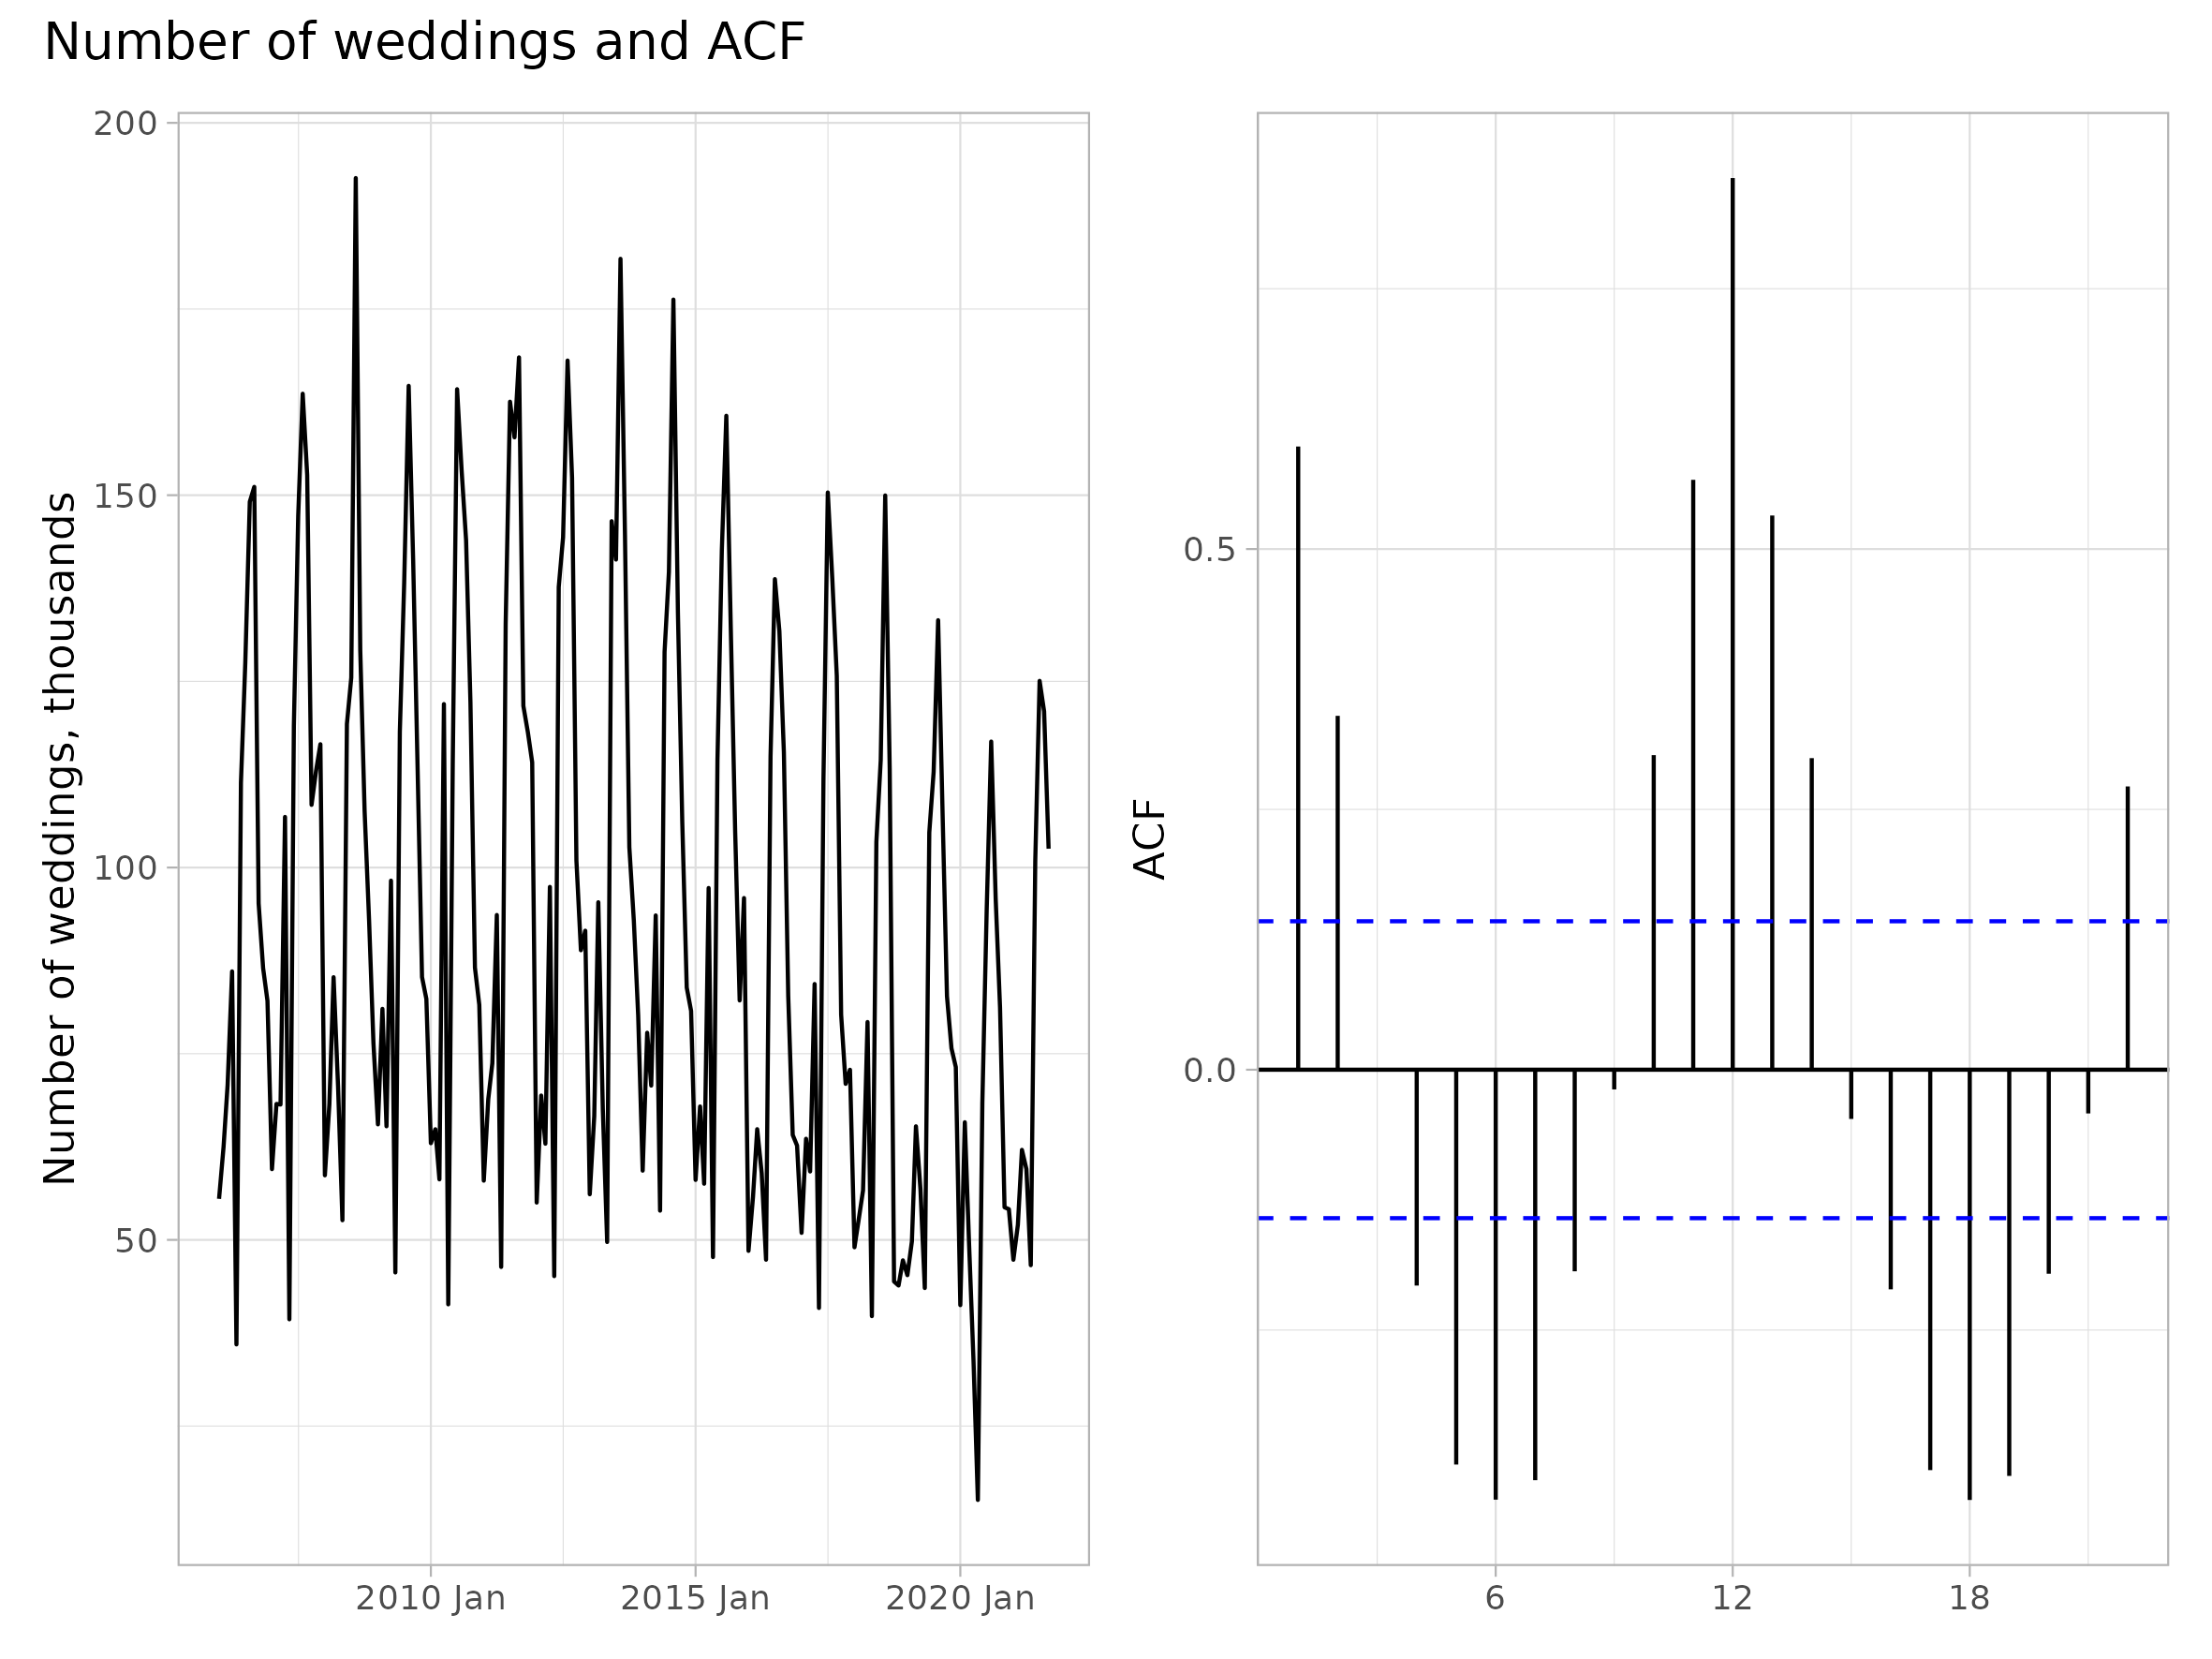
\includegraphics[width=\textwidth]{pictures/om_ts_01-120.png}
	
\end{frame}

\begin{frame}{Why is ACF a correlation?}
	
	\alert{Classic definition}
	
	\begin{block}{Sample ACF}
		$ACF_k$ — sample correlation between series $y_t$ and series $y_{t-k}$
	\end{block}
	
	\pause
	The difference between the definitions is \alert{small}
	
\end{frame}


\begin{frame}{PACF}
	
	\begin{block}{Sample PACF}
		Let's evaluate a set of multiple regressions:
		\[
		\hat y_t = \hat\alpha + \hat\beta_1 y_{t-1}, \quad PACF_1 = \hat\beta_1;
		\]
		\pause
		\[
		\hat y_t = \hat\alpha + \hat\beta_1 y_{t-1} + \hat\beta_2 y_{t-2}, \quad PACF_2 = \hat\beta_2;
		\]
		\pause
		\[
		\hat y_t = \hat\alpha + \hat\beta_1 y_{t-1} + \ldots + \hat\beta_k y_{t-k}, \quad PACF_k = \hat\beta_k
		\]
	\end{block}
	
	\pause
	\alert{Meaning}
	$PACF_2$: how many units is $y_t$ above average on average if $y_{t-2}$ is one unit above average,
	and $y_{t-1}$ is at the middle level
	
\end{frame}

\begin{frame}{Series and its PACF}
	
	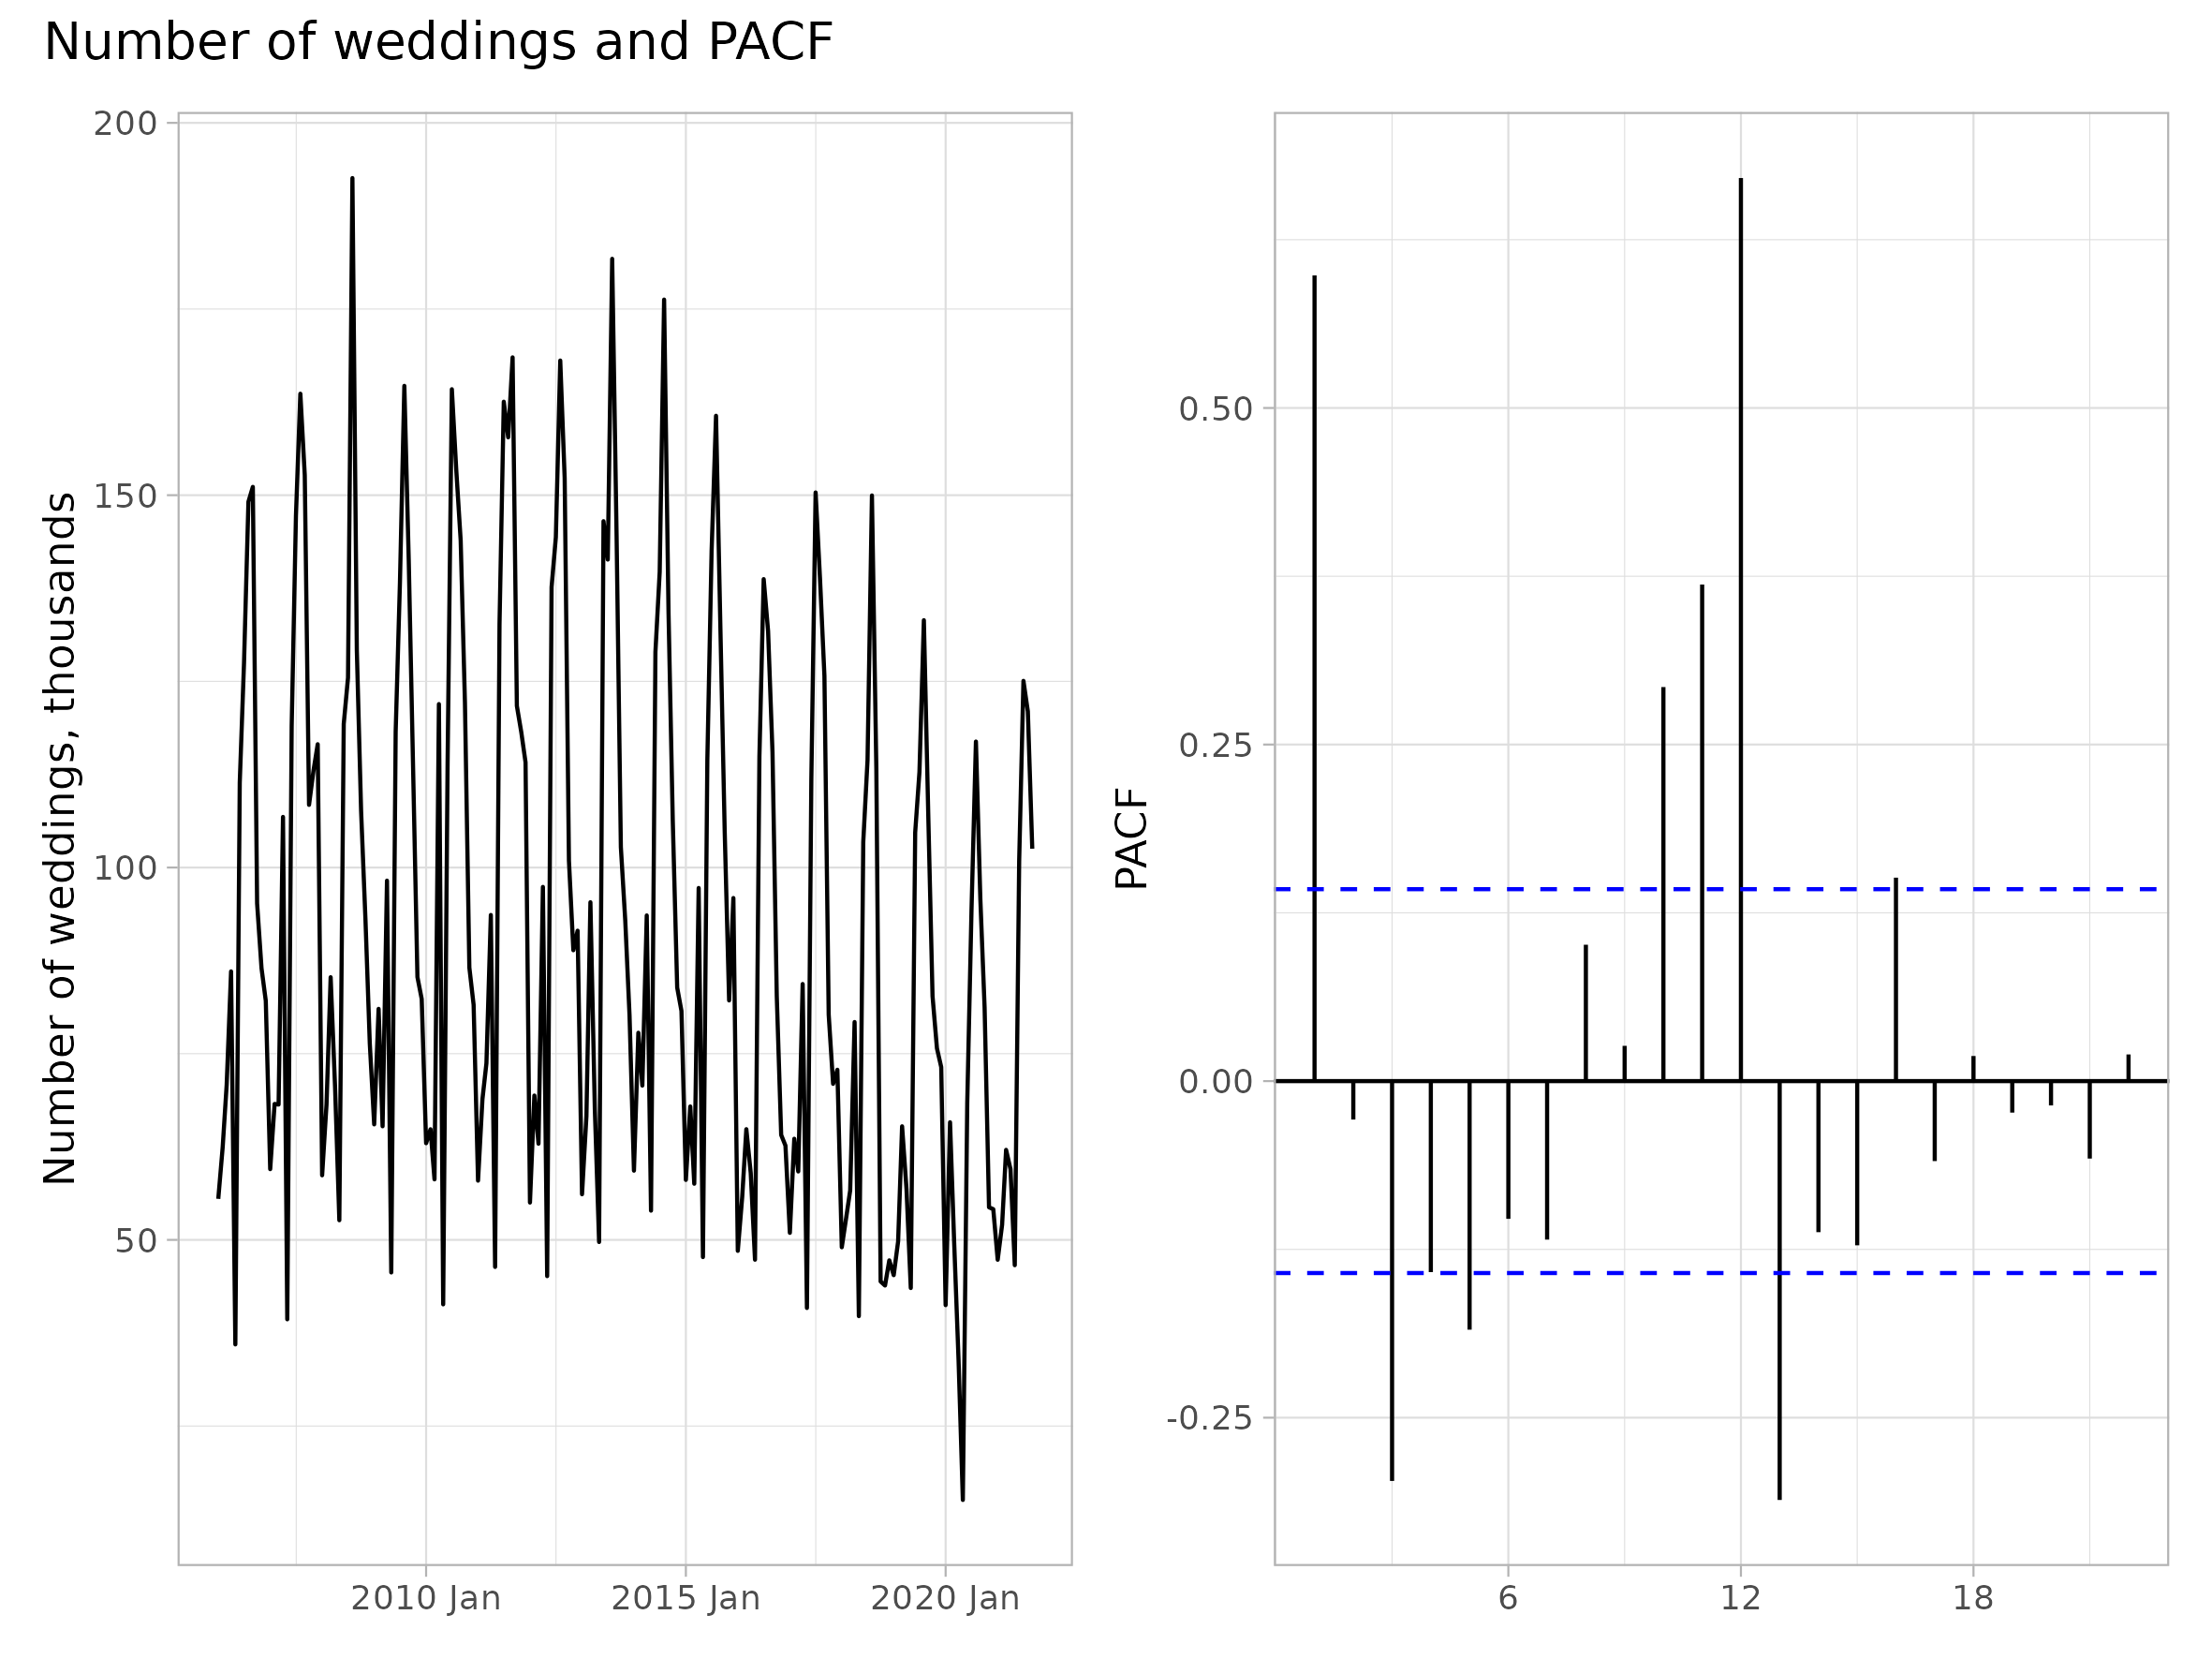
\includegraphics[width=\textwidth]{pictures/om_ts_01-127.png}
	
\end{frame}

\begin{frame}{Why is PACF a correlation?}
	
	\alert{Classic definition}
	
	\begin{block}{Custom PACF}
		$PACF_4$ — sample correlation between $a_t$ residuals and $b_t$ residuals:
		
		$a_t$ — regression residuals
		\[
		y_t \mid 1, y_{t-1}, y_{t-2}, y_{t-3};
		\]
		
		$b_t$ — regression residuals
		\[
		y_{t-4} \mid 1, y_{t-1}, y_{t-2}, y_{t-3}
		\]
	\end{block}
	
	\pause
	The difference between the definitions of \alert{small}
	
\end{frame}


\begin{frame}{STL features}
	
	\alert{Output:}
	\[
	y_t = T_t + S_t + R_t
	\]
	
	\pause
	Let's measure:
	\begin{itemize}
		\item Strength of $F_{trend}$ trend
		\item Strength of $F_{seas}$ seasonality
	\end{itemize}
	
\end{frame}

\begin{frame}{Strength of trend and seasonality}
	
	We got the decomposition:
	\[
	y_t = trend_t + seas_t + remainder_t.
	\]
	
	\pause
	\alert{Definition idea:}
	
	For an ideal decomposition with uncorrelated components:
	\[
	F_{trend} = \frac{\sVar(trend)}{\sVar(trend) + \sVar(remainder)},
	\]
	
	\pause
	\[
	F_{seas} = \frac{\sVar(seas)}{\sVar(seas) + \sVar(remainder)},
	\]
\end{frame}

\begin{frame}{Strength of trend and seasonality}
	
	We have the decomposition:
	\[
	y_t = trend_t + seas_t + remainder_t.
	\]
	
	\pause
	\alert{In practice}:
	\begin{itemize}[<+->]
		\item Trend strength:
		\[
		F_{trend} = \max\left\{1 - \frac{\sVar(remainder)}{\sVar(trend + remainder)}, 0 \right\}.
		\]
		\item Seasonality strength:
		\[
		F_{seas} = \max\left\{1 - \frac{\sVar(remainder)}{\sVar(seas + remainder)}, 0 \right\}.
		\]
		
	\end{itemize}
	
	
	
\end{frame}


\begin{frame}{Strength of trend and seasonality}
	
	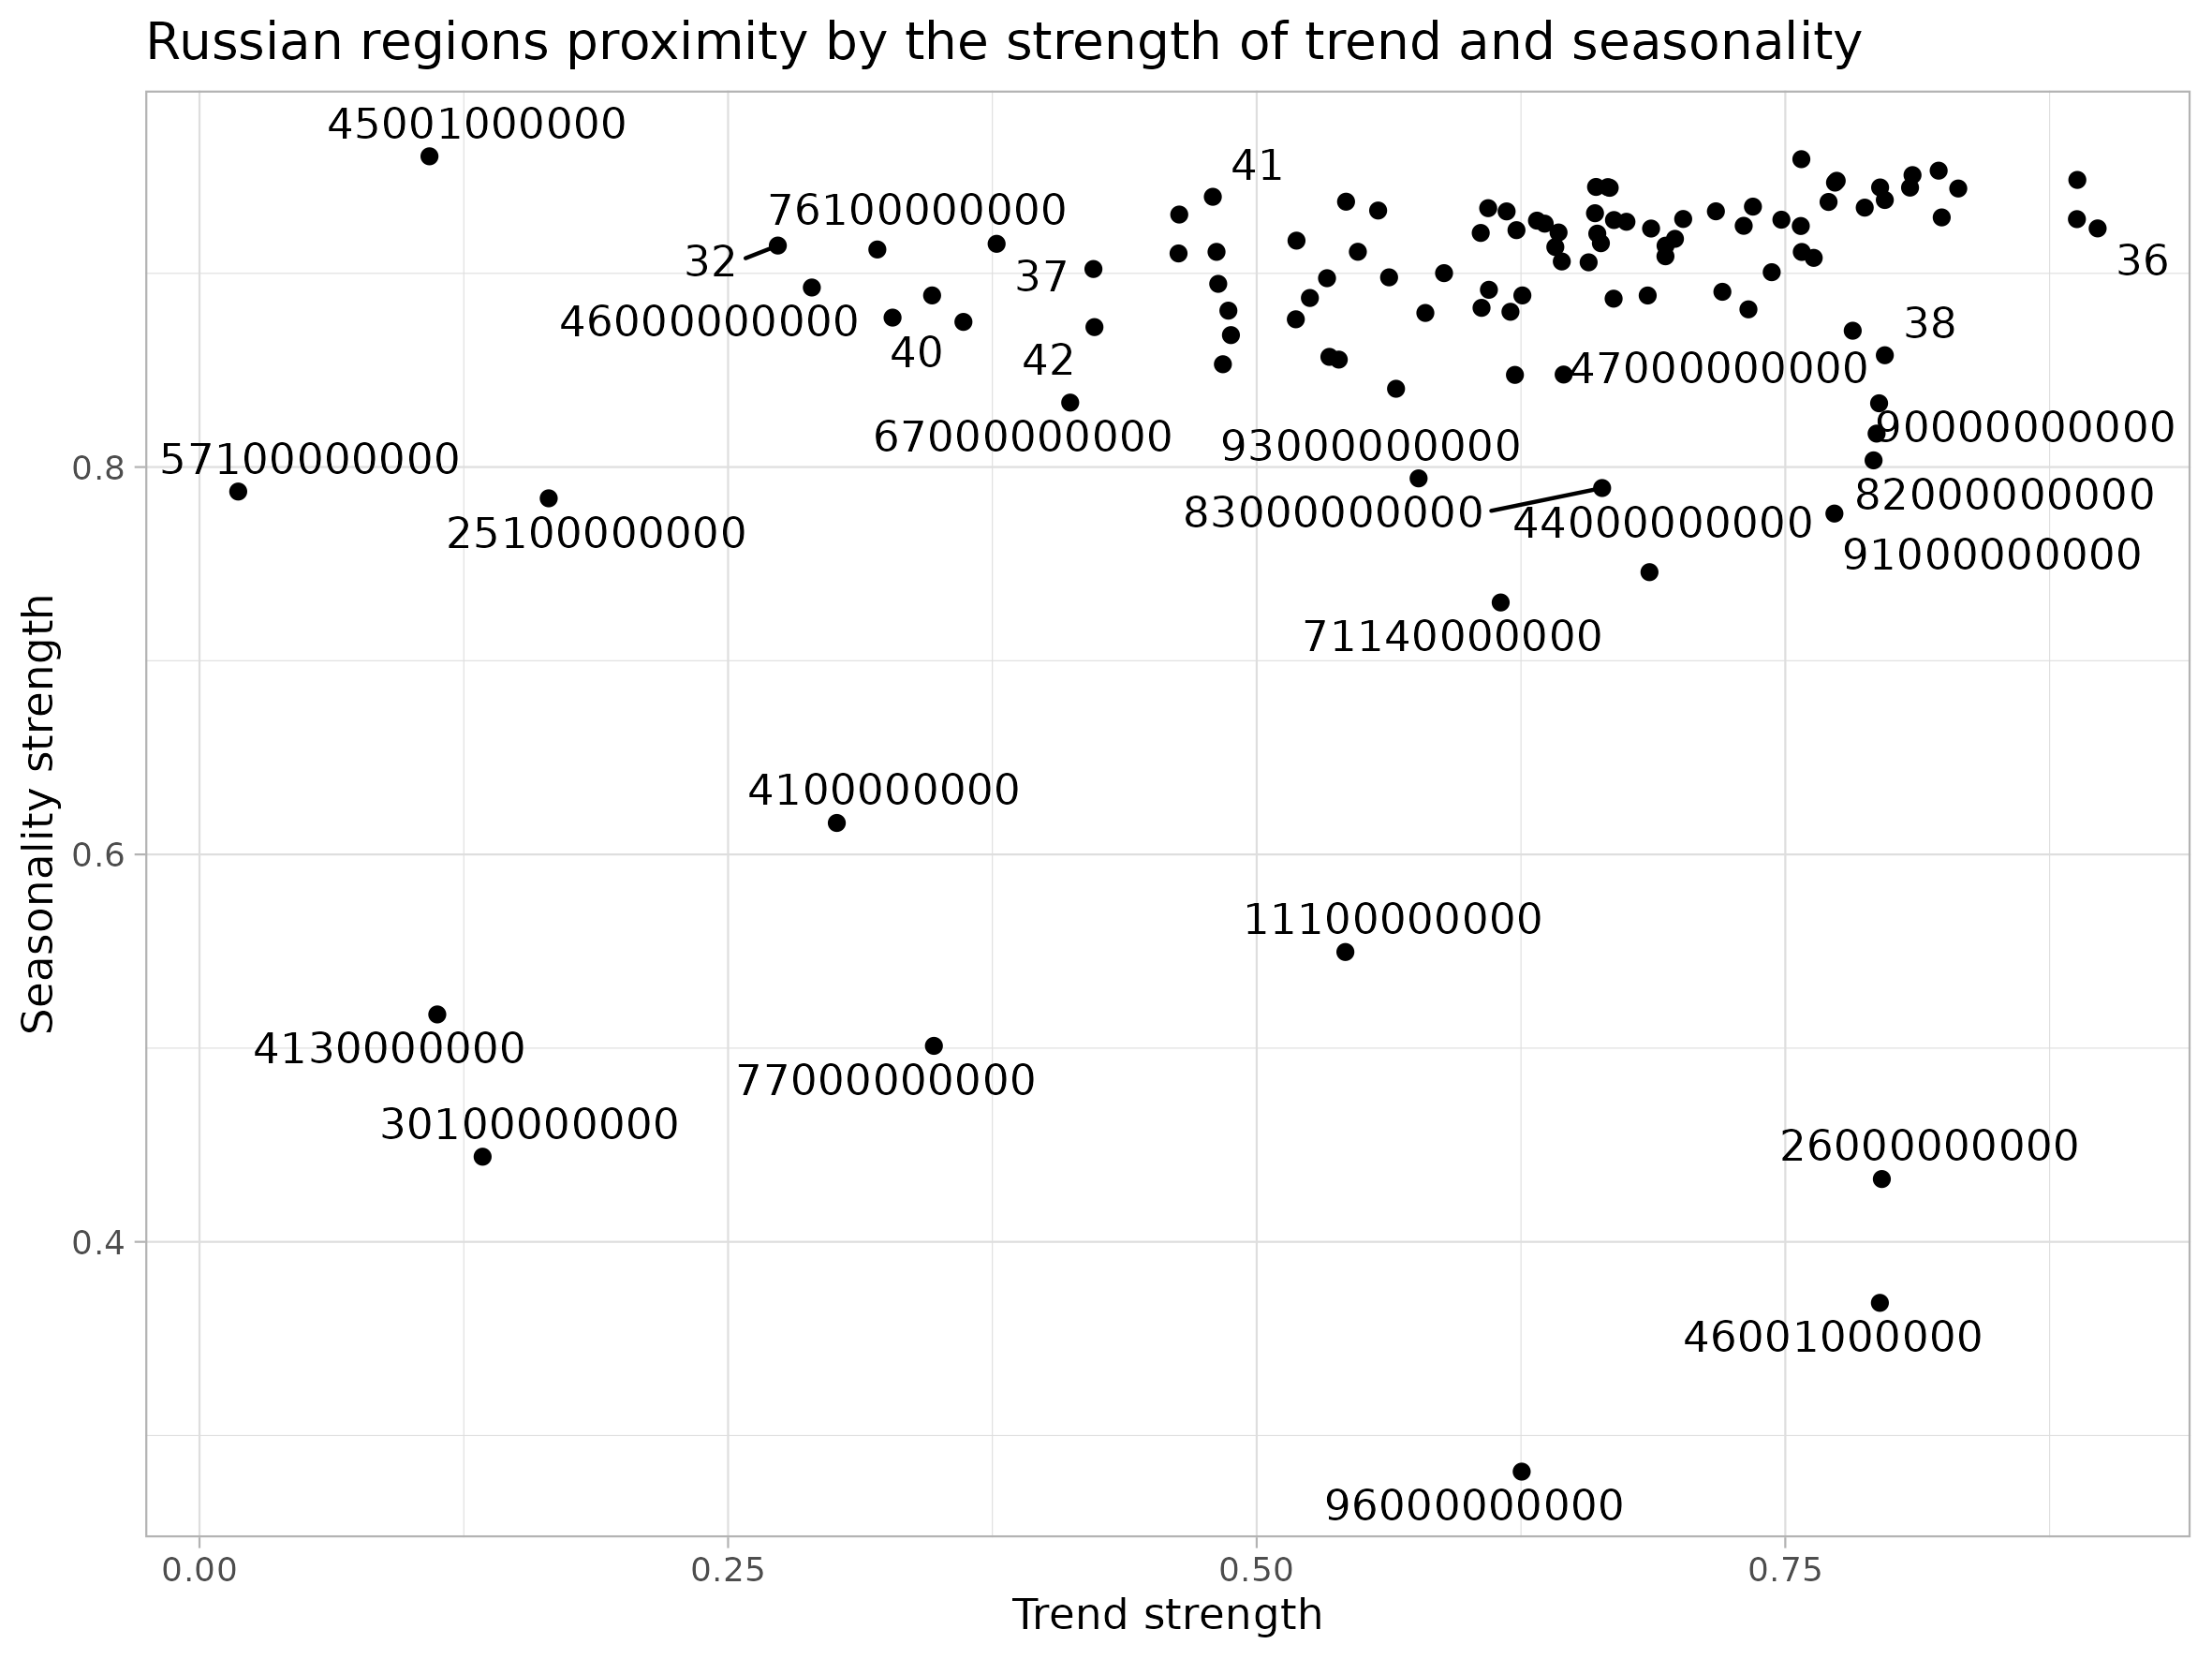
\includegraphics[width=\textwidth]{pictures/om_ts_01-138.png}
	
	
\end{frame}



\begin{frame}{Series Characteristics: Summary}
	
	\begin{itemize}[<+->]
		\item ACF — coefficients in \alert{paired} regressions or correlations
		\item PACF — coefficients in \alert{multiple} regressions or correlations
		\item STL allows you to measure \alert{strength of trend and seasonality} in comparison to the residual component
	\end{itemize}
\end{frame}


% !TEX root = ../om_ts_01.tex

\begin{frame} % frame name
	
	\videotitle{ETS Model (Part I)}
	
\end{frame}



\begin{frame}{ETS Model: Plan}
	\begin{itemize}[<+->]
		\item ETS as a model
		\item Formulas for predictions
		\item Adding a trend
		\item Idea of damped trend
	\end{itemize}
	
\end{frame}




\begin{frame}
	\frametitle{How many ETS models in total?}
	
	ETS — \alert{Error, Trend, Seasonality} (error, trend, seasonality)
	
	\pause
	
	\alert{Error}: A, M
	
	\alert{Trend}: N, A, Ad, M, Md
	
	\alert{Seasonality}: N, A, M
	
	\pause
	A — \alert{additive} component
	
	M — \alert{multiplicative} component
	
	N — no component
	
	d — \alert{damping} for the trend
	
	\pause
	
	Formally: \alert{30 options}
	
\end{frame}


\begin{frame}{Historical names}
	
	ETS(ANN) — simple exponential smoothing
	
	ETS(AAA) —  an additive Holt-Winters method
	
	ETS(AAM) —  the multiplicative Holt-Winters method
	
	ETS(AAdM) — Holt-Winters method with a fading trend
	
\end{frame}




\begin{frame}{ETS(ANN) terminology}
	
	$y_t$ — the observed series;
	
	$\ell_t$ — trend, cleaned series;
	
	$u_t$ — a random error
	
	\pause
	\[
	y_t = \ell_{t-1} + u_t;
	\]
	\pause
	\[
	\ell_t = \ell_{t-1} + \alpha u_t, \text{ starts at } \ell_0;
	\]
	\pause
	\[
	u_t \sim \dN(0;\sigma^2) \text{ and are independent}
	\]
	\pause
	
	Parameters: $\alpha$, $\sigma^2$, $\ell_0$
\end{frame}




\begin{frame}{Recognized?}
	
	ETS(ANN) is a generalization of \alert{random walk}
	\pause
	
	\[
	\begin{cases}
		y_t = \ell_{t-1} + u_t; \\
		\ell_t = \ell_{t-1} + \alpha u_t, \text{ starts at } \ell_0; \\
		u_t \sim \dN(0;\sigma^2) \text{ and are independent} \\
	\end{cases}
	\]
	
	\pause
	Substitute $\alpha = 1$:
	\[
	y_t = \ell_t = \ell_{t-1} + u_t
	\]
	
\end{frame}


\begin{frame}
	\frametitle{Estimation}
	
	\alert{Maximum likelihood method} is used for estimation
	
	\pause
	Main idea: \alert{decompose} the likelihood into a sum
	
	\begin{multline*}
		\ln L(y \mid \theta) = \ln L(y_1 \mid \theta) + \ln L(y_2 \mid y_1, \theta) + \ldots + \\
		+ \ln L(y_T \mid y_{T-1}, \ldots, y_1, \theta),
	\end{multline*}
	
	where $\theta = (\alpha, \ell_0, \sigma^2)$
	
	\pause
	Unfortunately, there are no explicit formulas for the estimators
	
\end{frame}

\begin{frame}
	\frametitle{Forecasting}
	
	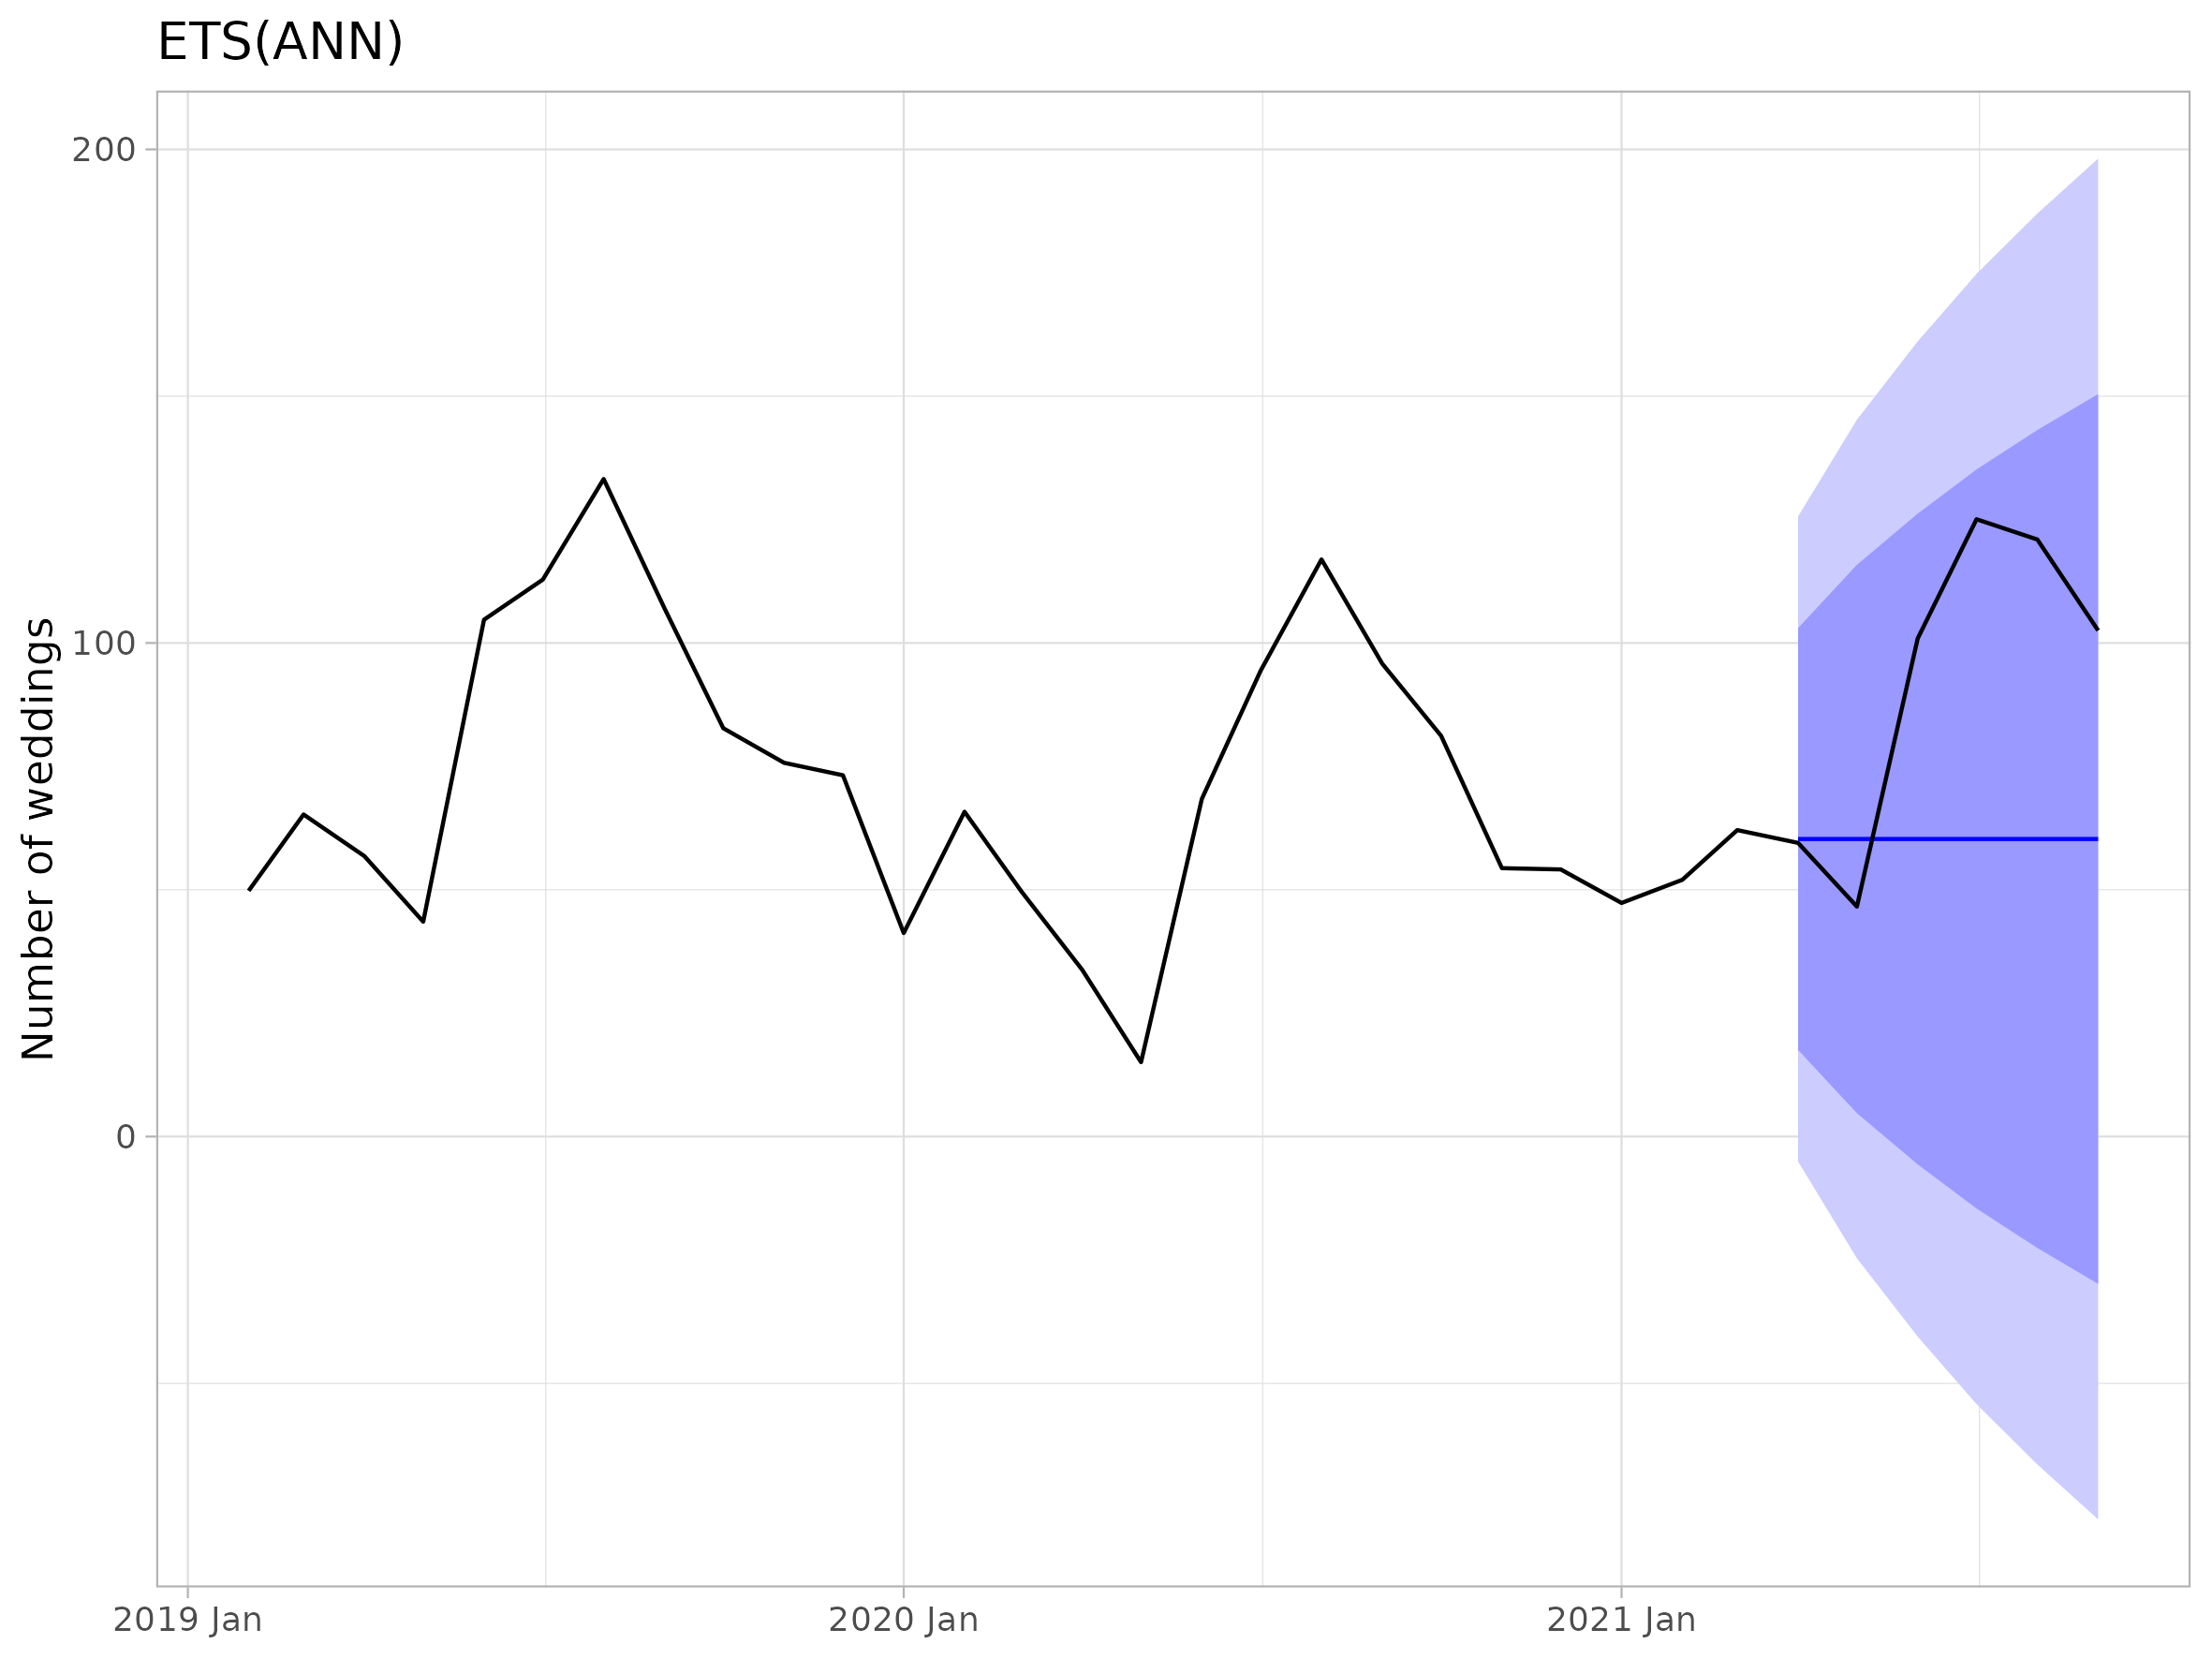
\includegraphics[width=\textwidth]{pictures/om_ts_02-025.png}
	
	
\end{frame}


\begin{frame}
	\frametitle{Forecast 1 step ahead}
	
	Luckily, there are \alert{recurrent formulas} for predictions
	\pause
	
	\[
	\begin{cases}
		y_t = \ell_{t-1} + u_t; \\
		\ell_t = \ell_{t-1} + \alpha u_t, \text{ starts at } \ell_0; \\
		u_t \sim \dN(0;\sigma^2) \text{ and are independent}\\
	\end{cases}
	\]
	\pause
	\[
	y_{T+1} = \ell_T + u_{T+1}
	\]
	\pause
	\[
	(y_{T+1} \mid \mathcal F_T) \sim \dN(\ell_T; \sigma^2)
	\]
	
\end{frame}


\begin{frame}
	\frametitle{Forecast 2 steps ahead}
	
	\[
	\begin{cases}
		y_t = \ell_{t-1} + u_t;\\
		\ell_t = \ell_{t-1} + \alpha u_t, \text{ starts at } \ell_0; \\
		u_t \sim \dN(0;\sigma^2) \text{ and are independent}\\
	\end{cases}
	\]
	\pause
	\[
	y_{T+2} = \ell_{T+1} + u_{T+2} = \ell_T + \alpha u_{T+1} + u_{T+2}
	\]
	\pause
	\[
	(y_{T+2} \mid \mathcal F_T) \sim \dN(\ell_T; \sigma^2(\alpha^2 + 1))
	\]
	
\end{frame}

\begin{frame}{Predictive intervals}
	
	From distribution law
	\[
	(y_{T+2} \mid \mathcal F_T) \sim \dN(\ell_T; \sigma^2(\alpha^2 + 1))
	\]
	we can derive a \pause \alert{predictive interval}
	\[
	[\hat\ell_T - 1.96 \hat\sigma \sqrt{\hat\alpha^2 + 1}; \hat \ell_T + 1.96 \hat\sigma \sqrt{\hat\alpha^2 + 1}].
	\]
\end{frame}


\begin{frame}
	\frametitle{What was discovered in the 1950s?}
	
	\[
	\begin{cases}
		y_t = \ell_{t-1} + u_t;\\
		\ell_t = \ell_{t-1} + \alpha u_t, \text{ starts at } \ell_0 \\
	\end{cases}
	\]
	\pause
	Let's rewrite the second equation:
	\[
	\ell_t = \ell_{t-1} + \alpha (y_t - \ell_{t-1}) = \alpha y_t + (1 - \alpha) \ell_{t-1}
	\]
	
	\pause
	\alert{Simple exponential smoothing}:
	
	\[
	\hat\ell_1 = y_1
	\]
	\pause
	\[
	\hat \ell_t = \alpha y_t + (1-\alpha) \hat \ell_{t-1}
	\]
	\pause
	\[
	\min_{\alpha} \sum (y_t - \hat \ell_t)^2
	\]
	
\end{frame}







\begin{frame}
	\frametitle{Adding trend!}
	
	$y_t$ — the observed series;
	
	$\ell_t$ — trend, cleaned series;
	
	$b_t$ — current growth rate of the cleaned series;
	
	$u_t$ — a random error
	
	\pause
	ETS(AAN):
	
	A — \alert{additive} error;
	
	A — \alert{additive} trend;
	
	N — \alert{no} seasonality
	
\end{frame}

\begin{frame}
	\frametitle{ETS(AAN): equations}
	
	
	\[
	\begin{cases}
		y_t = \ell_{t-1} + \alert{b_{t-1}} + u_t; \\
		\ell_t = \ell_{t-1} + \alert{b_{t-1}} + \alpha u_t, \text{ starts at } \ell_0; \\
		u_t \sim \dN(0;\sigma^2) \text{ and are independent} \\
		\alert{b_t = b_{t-1} + \beta u_t},\text{ starts at } b_0; \\
	\end{cases}
	\]
	
	
	Parameters: $\alpha$, $\beta$, $\sigma^2$, $\ell_0$, $b_0$
	
	
\end{frame}

\begin{frame}
	\frametitle{ETS(AAN): Forecasting}
	
	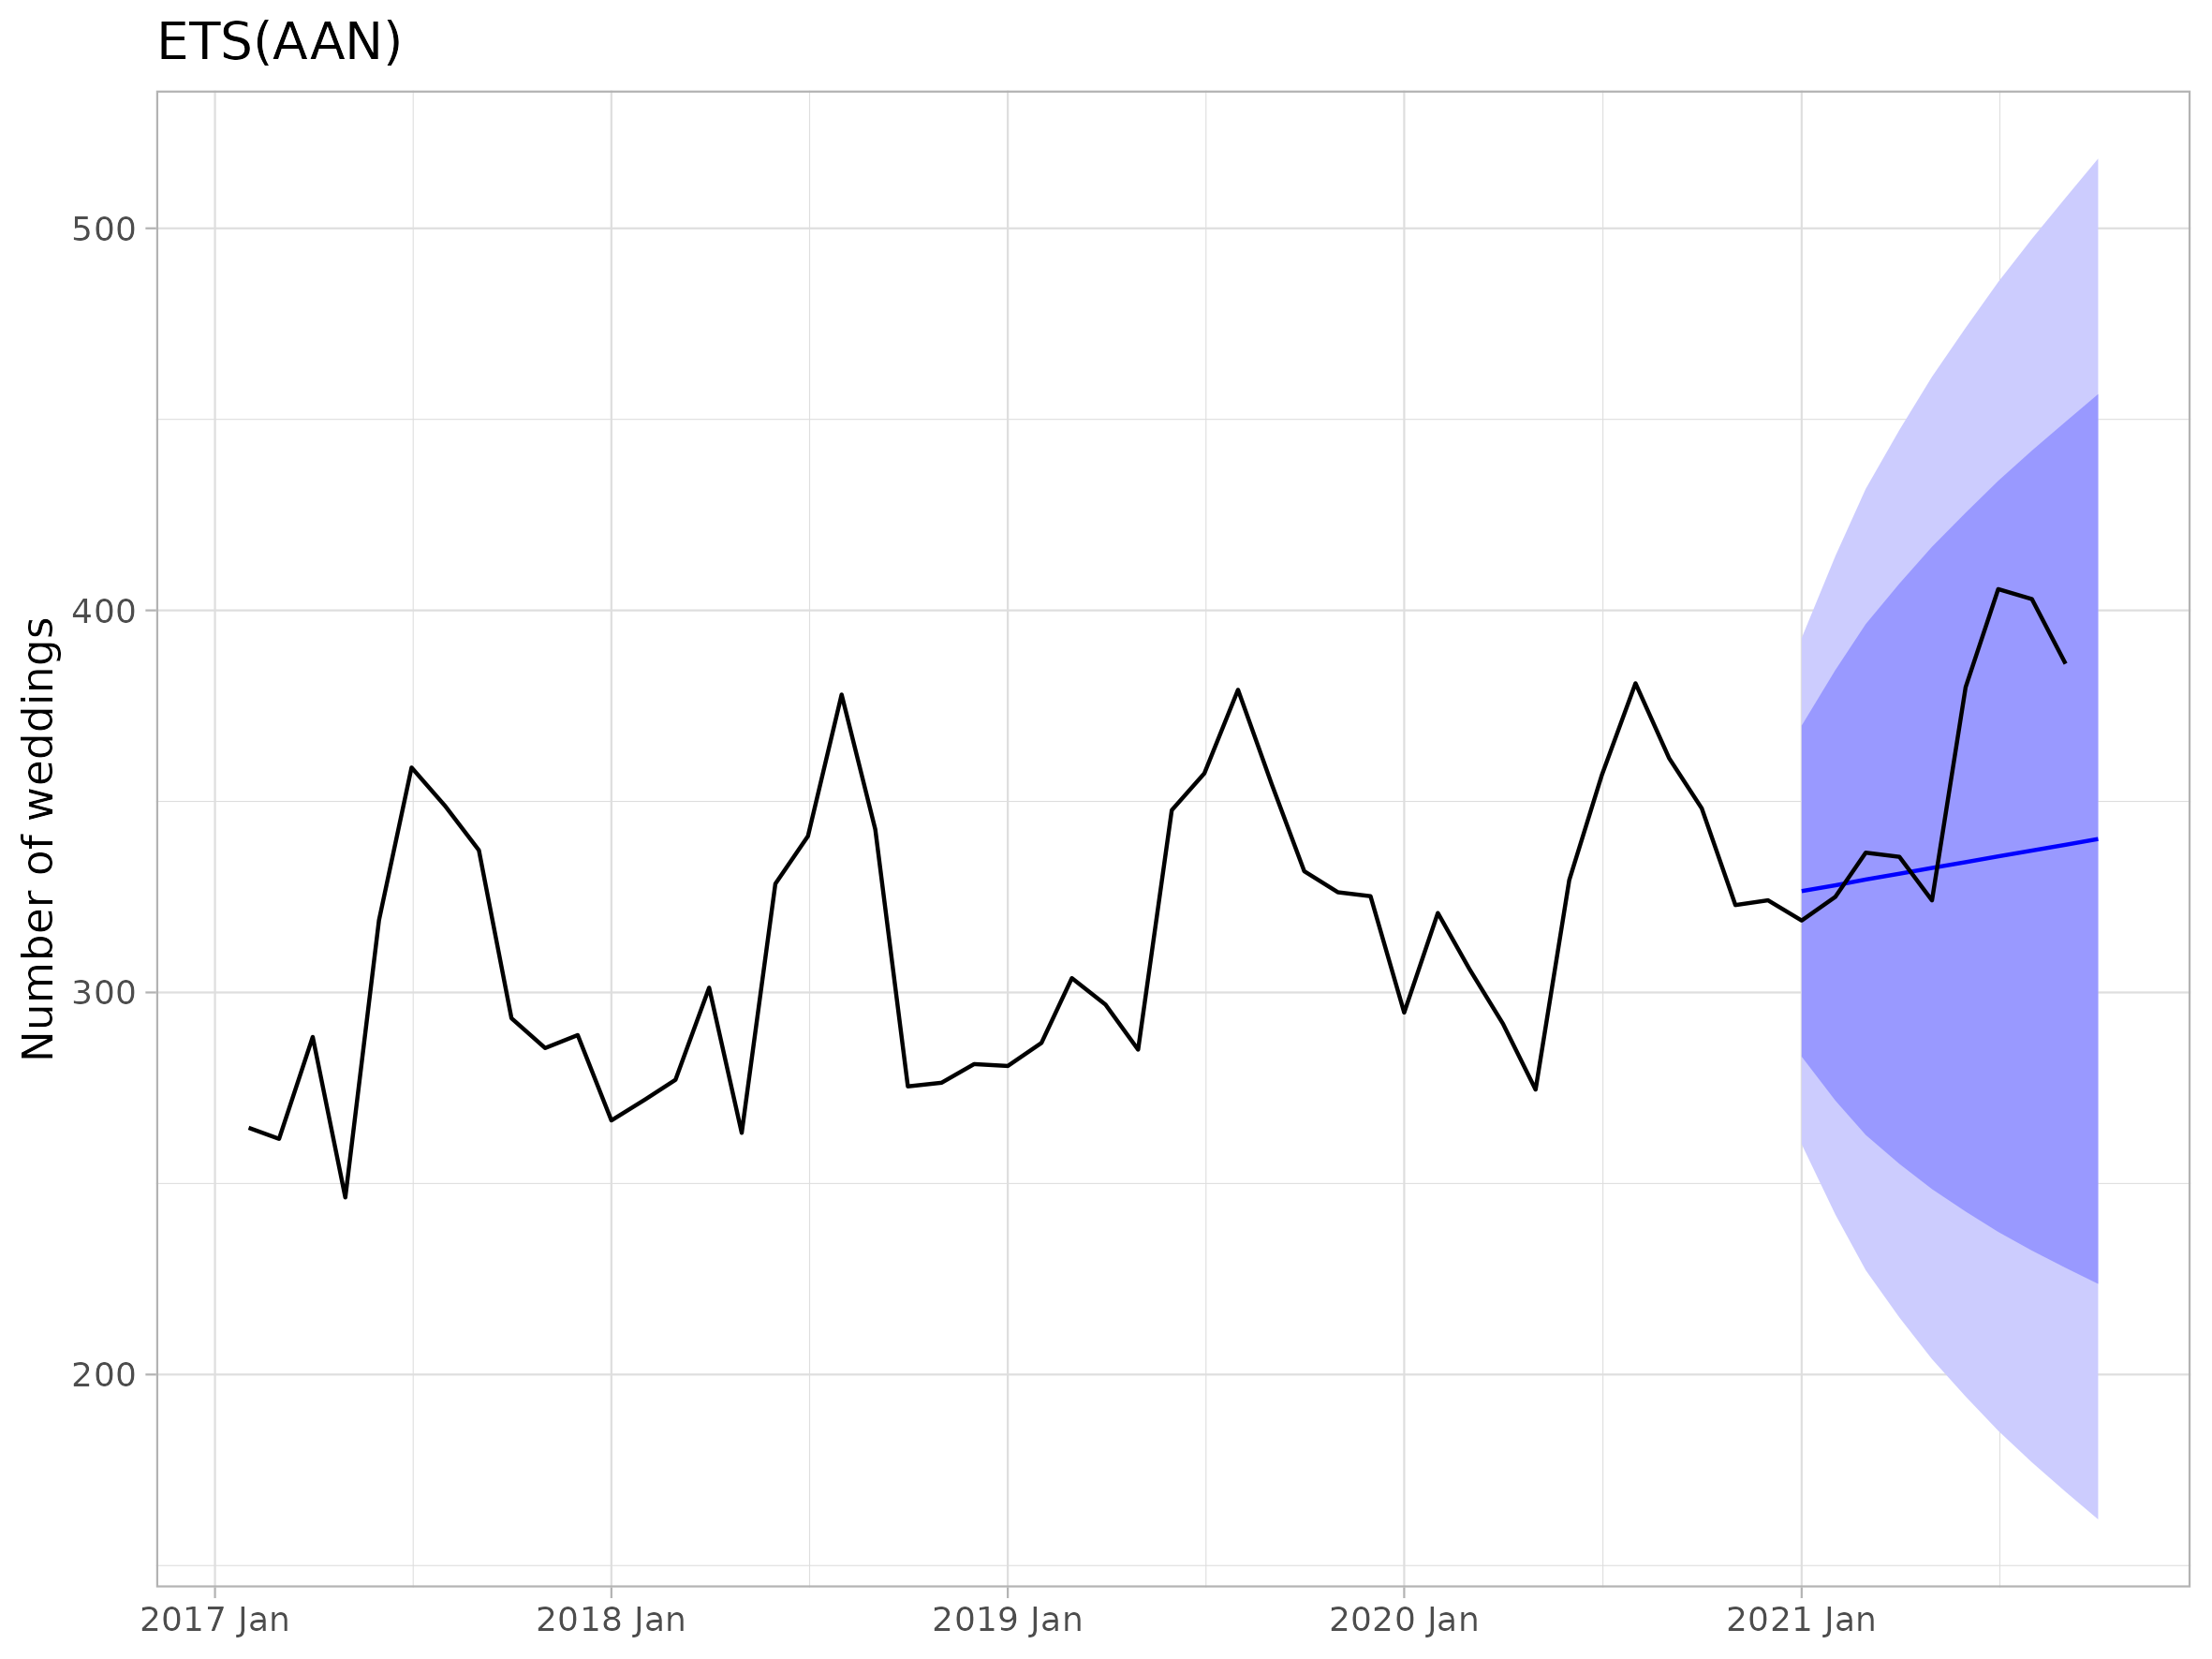
\includegraphics[width=\textwidth]{pictures/om_ts_02-052.png}
	
\end{frame}


\begin{frame}
	\frametitle{Forecast 1 step ahead}
	
	\[
	\begin{cases}
		y_t = \ell_{t-1} + b_{t-1} + u_t; \\
		\ell_t = \ell_{t-1} + b_{t-1} + \alpha u_t, \text{ starts at } \ell_0; \\
		u_t \sim \dN(0;\sigma^2) \text{ and are independent.} \\
		b_t = b_{t-1} + \beta u_t,\text{ starts at } b_0 \\
	\end{cases}
	\]
	
	\[
	y_{T+1} = \ell_T + b_T + u_{T+1}
	\]
	
	\[
	(y_{T+1} \mid \mathcal F_T) \sim \dN(\ell_T + b_T; \sigma^2)
	\]
	
\end{frame}


\begin{frame}
	\frametitle{Forecast 2 steps ahead}
	
	\[
	\begin{cases}
		y_t = \ell_{t-1} + b_{t-1} + u_t; \\
		\ell_t = \ell_{t-1} + b_{t-1} + \alpha u_t, \text{ starts at } \ell_0; \\
		u_t \sim \dN(0;\sigma^2) \text{ and are independent} \\
		b_t = b_{t-1} + \beta u_t,\text{ starts at } b_0 \\
	\end{cases}
	\]
	
	\begin{multline*}
		y_{T+2} = \ell_{T+1} + b_{T+1} + u_{T+2} = (\ell_T + b_T + \alpha u_{T+1}) +\\
		+ (b_T + \beta u_{T+1}) + u_{T+2}
	\end{multline*}
	
	\[
	(y_{T+2} \mid \mathcal F_T) \sim \dN(\ell_T + 2b_T; \sigma^2((\alpha + \beta)^2 + 1))
	\]
	
\end{frame}



\begin{frame}{Problem with trend in ETS(AAN)}
	
	In the ETS(AAN) model \alert{growth rate} of the $\ell_t$ trend is defined by the formula
	\[
	b_t = b_{t-1} + \beta u_t, \text{ starts at } b_0
	\]
	\pause
	Consequently,
	\[
	\E(b_t) = \E(b_{t-1}), \quad \E(b_{T+h} \mid b_T) = b_T
	\]
	\pause
	Long-term forecast of a positive indicator at $b_T < 0$
	will become negative
\end{frame}

\begin{frame}{Contradiction}
	In short-term we expect a change in the indicator:
	
	we \alert{ want a trend} in the model.
	
	\pause
	In long-term negative values are impossible:
	
	we  \alert{don't want a trend} in the model.
	
	\pause
	Solution: \alert{damped} or \alert{fading} trend.
\end{frame}

\begin{frame}{Extra parameters are expensive!}
	We want richer trend dynamics — we need \alert{additional} parameters.
	
	\pause
	Additional parameters — risk \alert{overfitting} of the model,
	\alert{wider confidence intervals} for the remaining parameters.
	
	\pause
	Let's solve the problem  with only \alert{one} new parameter!
\end{frame}

\begin{frame}
	\frametitle{Damped trend}
	
	We introduce the trend damping parameter $\phi \in (0; 1)$ into the slope equation:
	\[
	b_t = \phi b_{t-1} + \beta u_t, \text{ starts at } b_0
	\]
	\pause
	And for the rest of the equations:
	\[
	\begin{cases}
		y_t = \ell_{t-1} + \phi b_{t-1} + u_t; \\
		\ell_t = \ell_{t-1} + \phi b_{t-1} + \alpha u_t, \text{ starts at } \ell_0\\
	\end{cases}
	\]
	
\end{frame}


\begin{frame}{General form of ETS(AAdN)}
	
	\[
	\begin{cases}
		y_t = \ell_{t-1} + \phi b_{t-1} + u_t; \\
		\ell_t = \ell_{t-1} + \phi b_{t-1} + \alpha u_t, \text{ starts at } \ell_0; \\
		b_t = \phi b_{t-1} + \beta u_t, \text{ starts at } b_0; \\
		u_t \sim \dN(0;\sigma^2) \text{ and are independent} \\
	\end{cases}
	\]
	
	
	
	Parameters: $\alpha$, $\sigma^2$, $\ell_0$, $b_0$, $\beta$, $\phi$
\end{frame}

\begin{frame}
	\frametitle{ETS(AAdN): Forecasting}
	
	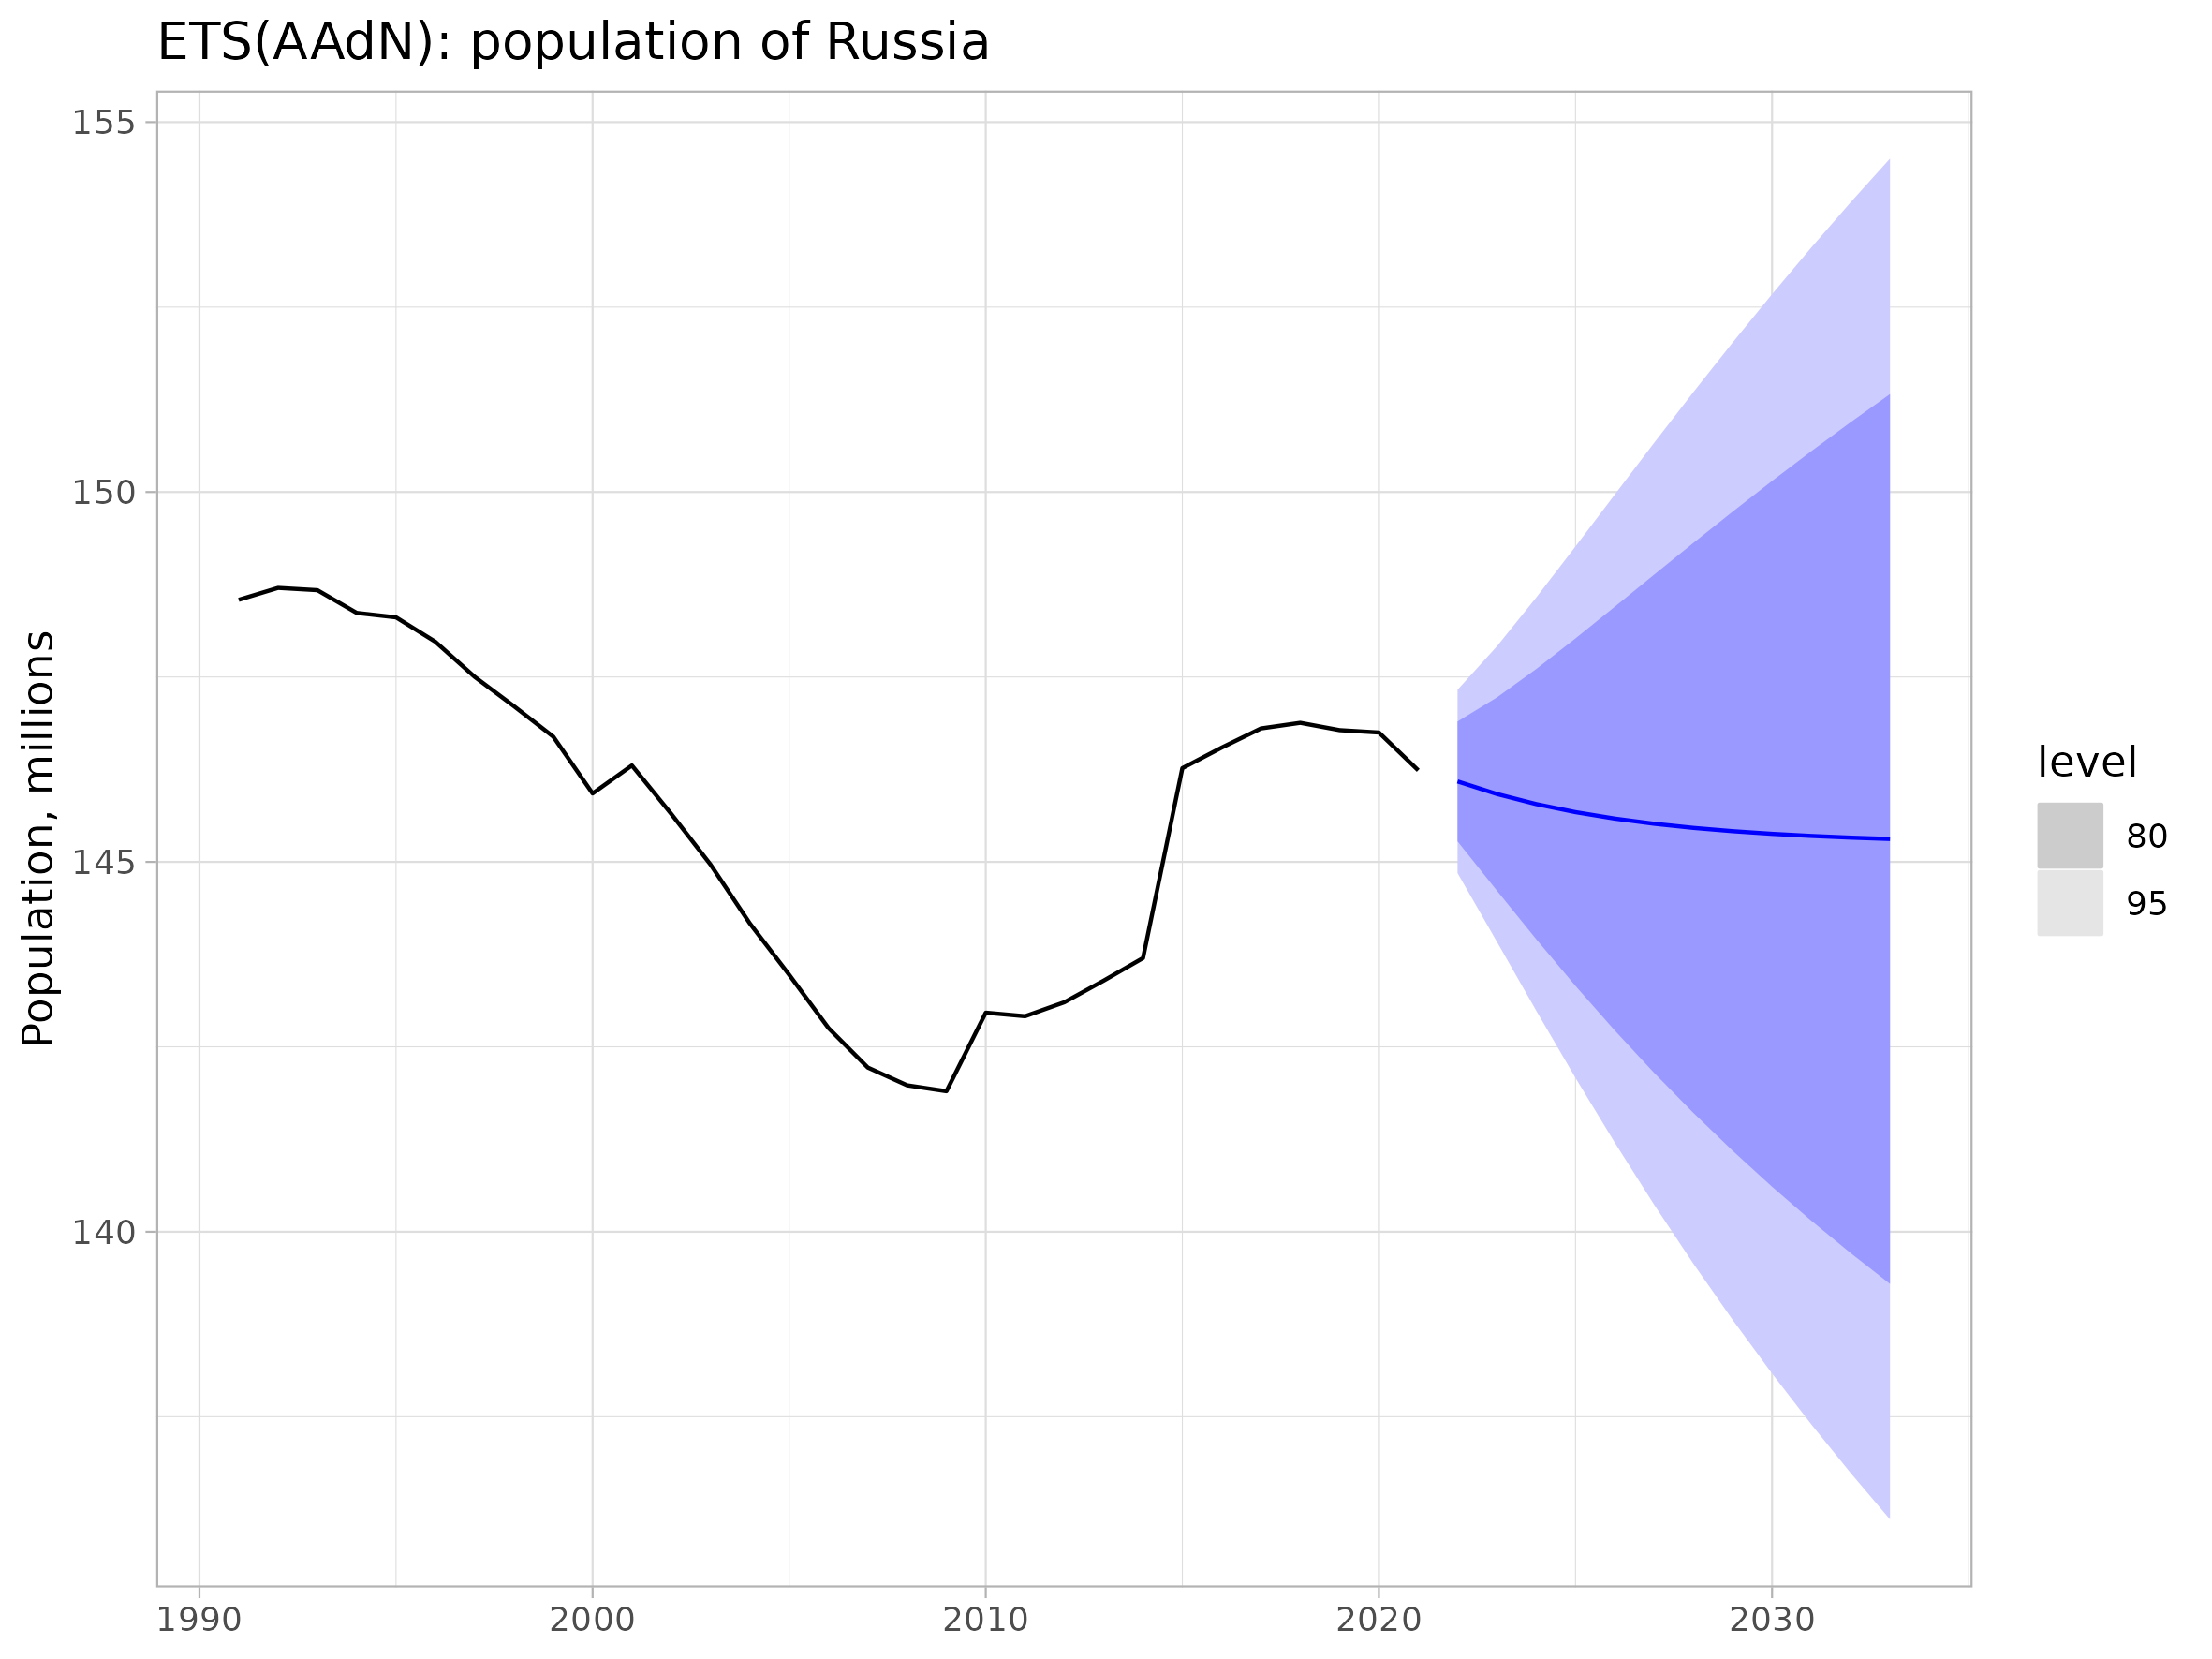
\includegraphics[width=\textwidth]{pictures/om_ts_03-019.png}
	
	% https://www.youtube.com/watch?v=e5WxxvjR9c4
	% I can’t understand what the secret is, if there is a trend, then it doesn’t exist right away.
	
\end{frame}





\begin{frame}{ETS Model: Summary}
	
	\begin{itemize}[<+->]
		\item Formulas for \alert{exponential smoothing} have been around for a long time
		\item ETS — a wide class of modern models
		\item The slope of the trend line can change
		\item Damped trend: on a small forecasting horizon \alert{there is a trend}, on a large horizon — \alert{none}
		
	\end{itemize}
\end{frame}







\begin{frame} % frame name
	
	\videotitle{ETS Model (Part II)}
	
\end{frame}



\begin{frame}{ETS Model: Plan}
	\begin{itemize}[<+->]
		\item Adding seasonality
		\item Formulas for predictions
		\item Decomposition into components
		
		\item Multiplicative components
	\end{itemize}
	
\end{frame}









\begin{frame}
	\frametitle{Adding seasonality!}
	
	$y_t$ — the observed series;
	
	$\ell_t$ — trend, cleaned series;
	
	$b_t$ — current growth rate of the cleaned series;
	
	$s_t$ — seasonal component;
	
	$u_t$ — a random error
	
	\pause
	ETS(AAA):
	
	A — \alert{additive} error;
	
	A — \alert{additive} trend;
	
	A — \alert{additive} seasonality
	
\end{frame}


% TODO: typo with u_t correct on slides!
\begin{frame}
	\frametitle{ETS(AAA): equations}
	
	
	\[
	\begin{cases}
		y_t = \ell_{t-1} + b_{t-1} + \alert{s_{t-12}} + u_t; \\
		\ell_t = \ell_{t-1} + b_{t-1} + \alpha u_t, \text{ starts at } \ell_0; \\
		u_t \sim \dN(0;\sigma^2) \text{ and are independent} \\
		b_t = b_{t-1} + \beta u_t,\text{ starts at } b_0; \\
		\alert{s_t = s_{t-12} + \gamma u_t}; \text{ starts at} s_0, s_{-1}, \ldots, s_{-11}
	\end{cases}
	\]
	
	
	Parameters: $\alpha$, $\beta$, $\gamma$, $\sigma^2$, $\ell_0$, $b_0$, $s_0$, $s_{-1}$, \ldots, $s_ {-11}$
	
	\alert{Restriction}: $s_0 + s_{-1} + \ldots + s_{-11} = 0$
	
	\pause
	
	How many independent parameters are we estimating?
	
	\pause
	
	Correct answer: 17
	
	
\end{frame}



\begin{frame}
	\frametitle{ETS(AAA): Forecasting}
	
	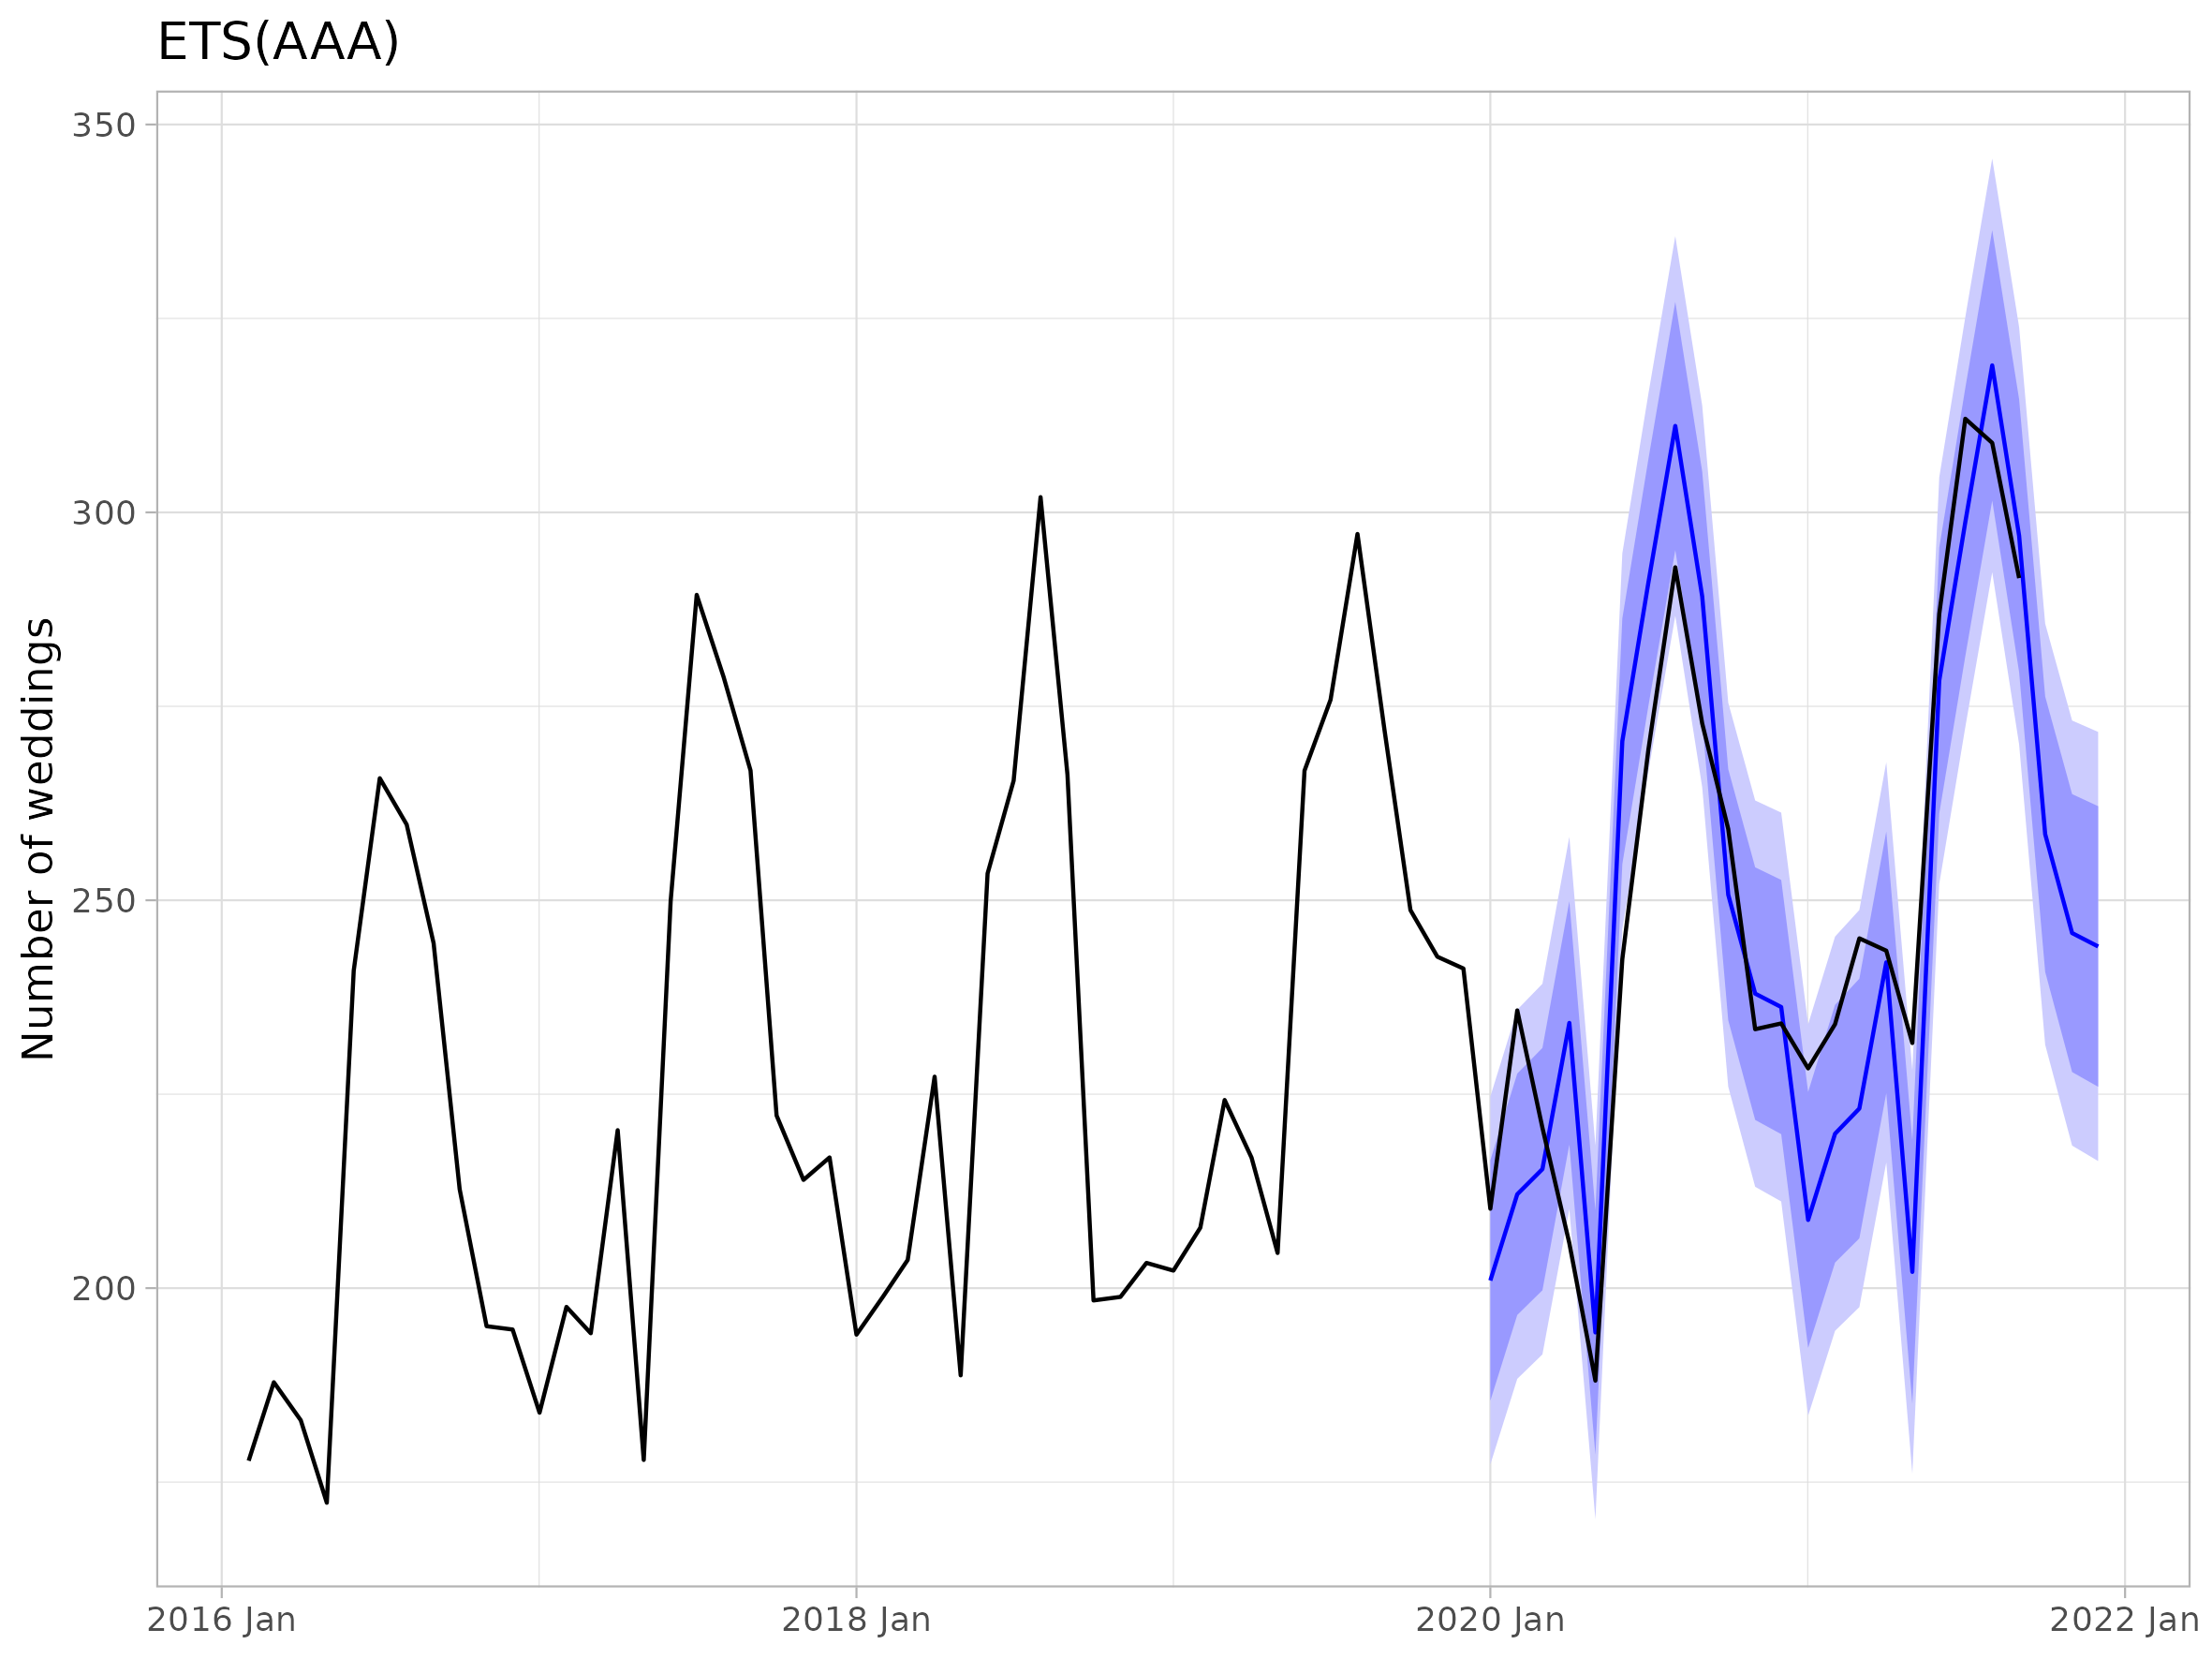
\includegraphics[width=\textwidth]{pictures/om_ts_02-076.png}
	
	
\end{frame}


\begin{frame}
	\frametitle{Forecast 1 step ahead}
	
	\[
	\begin{cases}
		y_t = \ell_{t-1} + b_{t-1} + s_{t-12} + u_t; \\
		\ell_t = \ell_{t-1} + b_{t-1} + \alpha u_t, \text{ starts at } \ell_0; \\
		u_t \sim \dN(0;\sigma^2) \text{ and are independent.} \\
		b_t = b_{t-1} + \beta u_t,\text{ starts at } b_0; \\
		s_t = s_{t-12} + \gamma u_t
	\end{cases}
	\]
	
	\[
	y_{T+1} = \ell_T + b_T + s_{T-11} + u_{T+1}
	\]
	
	\[
	(y_{T+1} \mid \mathcal F_T) \sim \dN(\ell_T + b_T + s_{T-11}; \sigma^2)
	\]
	
\end{frame}


\begin{frame}
	\frametitle{Forecast 2 steps ahead}
	
	\[
	\begin{cases}
		y_t = \ell_{t-1} + b_{t-1} + s_{t-12} + u_t; \\
		\ell_t = \ell_{t-1} + b_{t-1} + \alpha u_t, \text{ starts at } \ell_0; \\
		u_t \sim \dN(0;\sigma^2) \text{ and are independent} \\
		b_t = b_{t-1} + \beta u_t,\text{ starts at } b_0; \\
		s_t = s_{t-12} + \gamma u_t
	\end{cases}
	\]
	
	\begin{multline*}
		y_{T+2} = \ell_{T+1} + b_{T+1} + s_{T-10} + u_{T+2} = (\ell_T + b_T + \alpha u_{T+1} ) +\\
		+ (b_T + \beta u_{T+1}) + s_{T-10} + u_{T+2}
	\end{multline*}
	
	\[
	(y_{T+2} \mid \mathcal F_T) \sim \dN(\ell_T + 2b_T + s_{T-10}; \sigma^2((\alpha + \beta)^2 + 1))
	\]
	
\end{frame}




\begin{frame}
	\frametitle{Decomposition for free!}
	
	Consider the output of ETS(AAA):
	
	\alert{Parameter estimates}: $\hat\alpha$, $\hat\beta$, $\hat\gamma$, $\hat\sigma^2$, $\hat\ell_0$, $\hat b_0$,
	$\hat s_0$, $\hat s_{-1}$, \ldots, $\hat s_{-11}$.
	
	Constraints: $\hat s_0 + \hat s_{-1} + \ldots + \hat s_{-11} = 0$.
	
	\pause
	Estimated \alert{component values}: $\hat \ell_t$, $\hat b_t$, $\hat s_t$.
	
	\pause
	We automatically get \alert{decomposition}: $y_t = \hat \ell_t + \hat s_t + remainder_t$.
	
\end{frame}











\begin{frame}
	\frametitle{Oscillation amplitude can vary}
	
	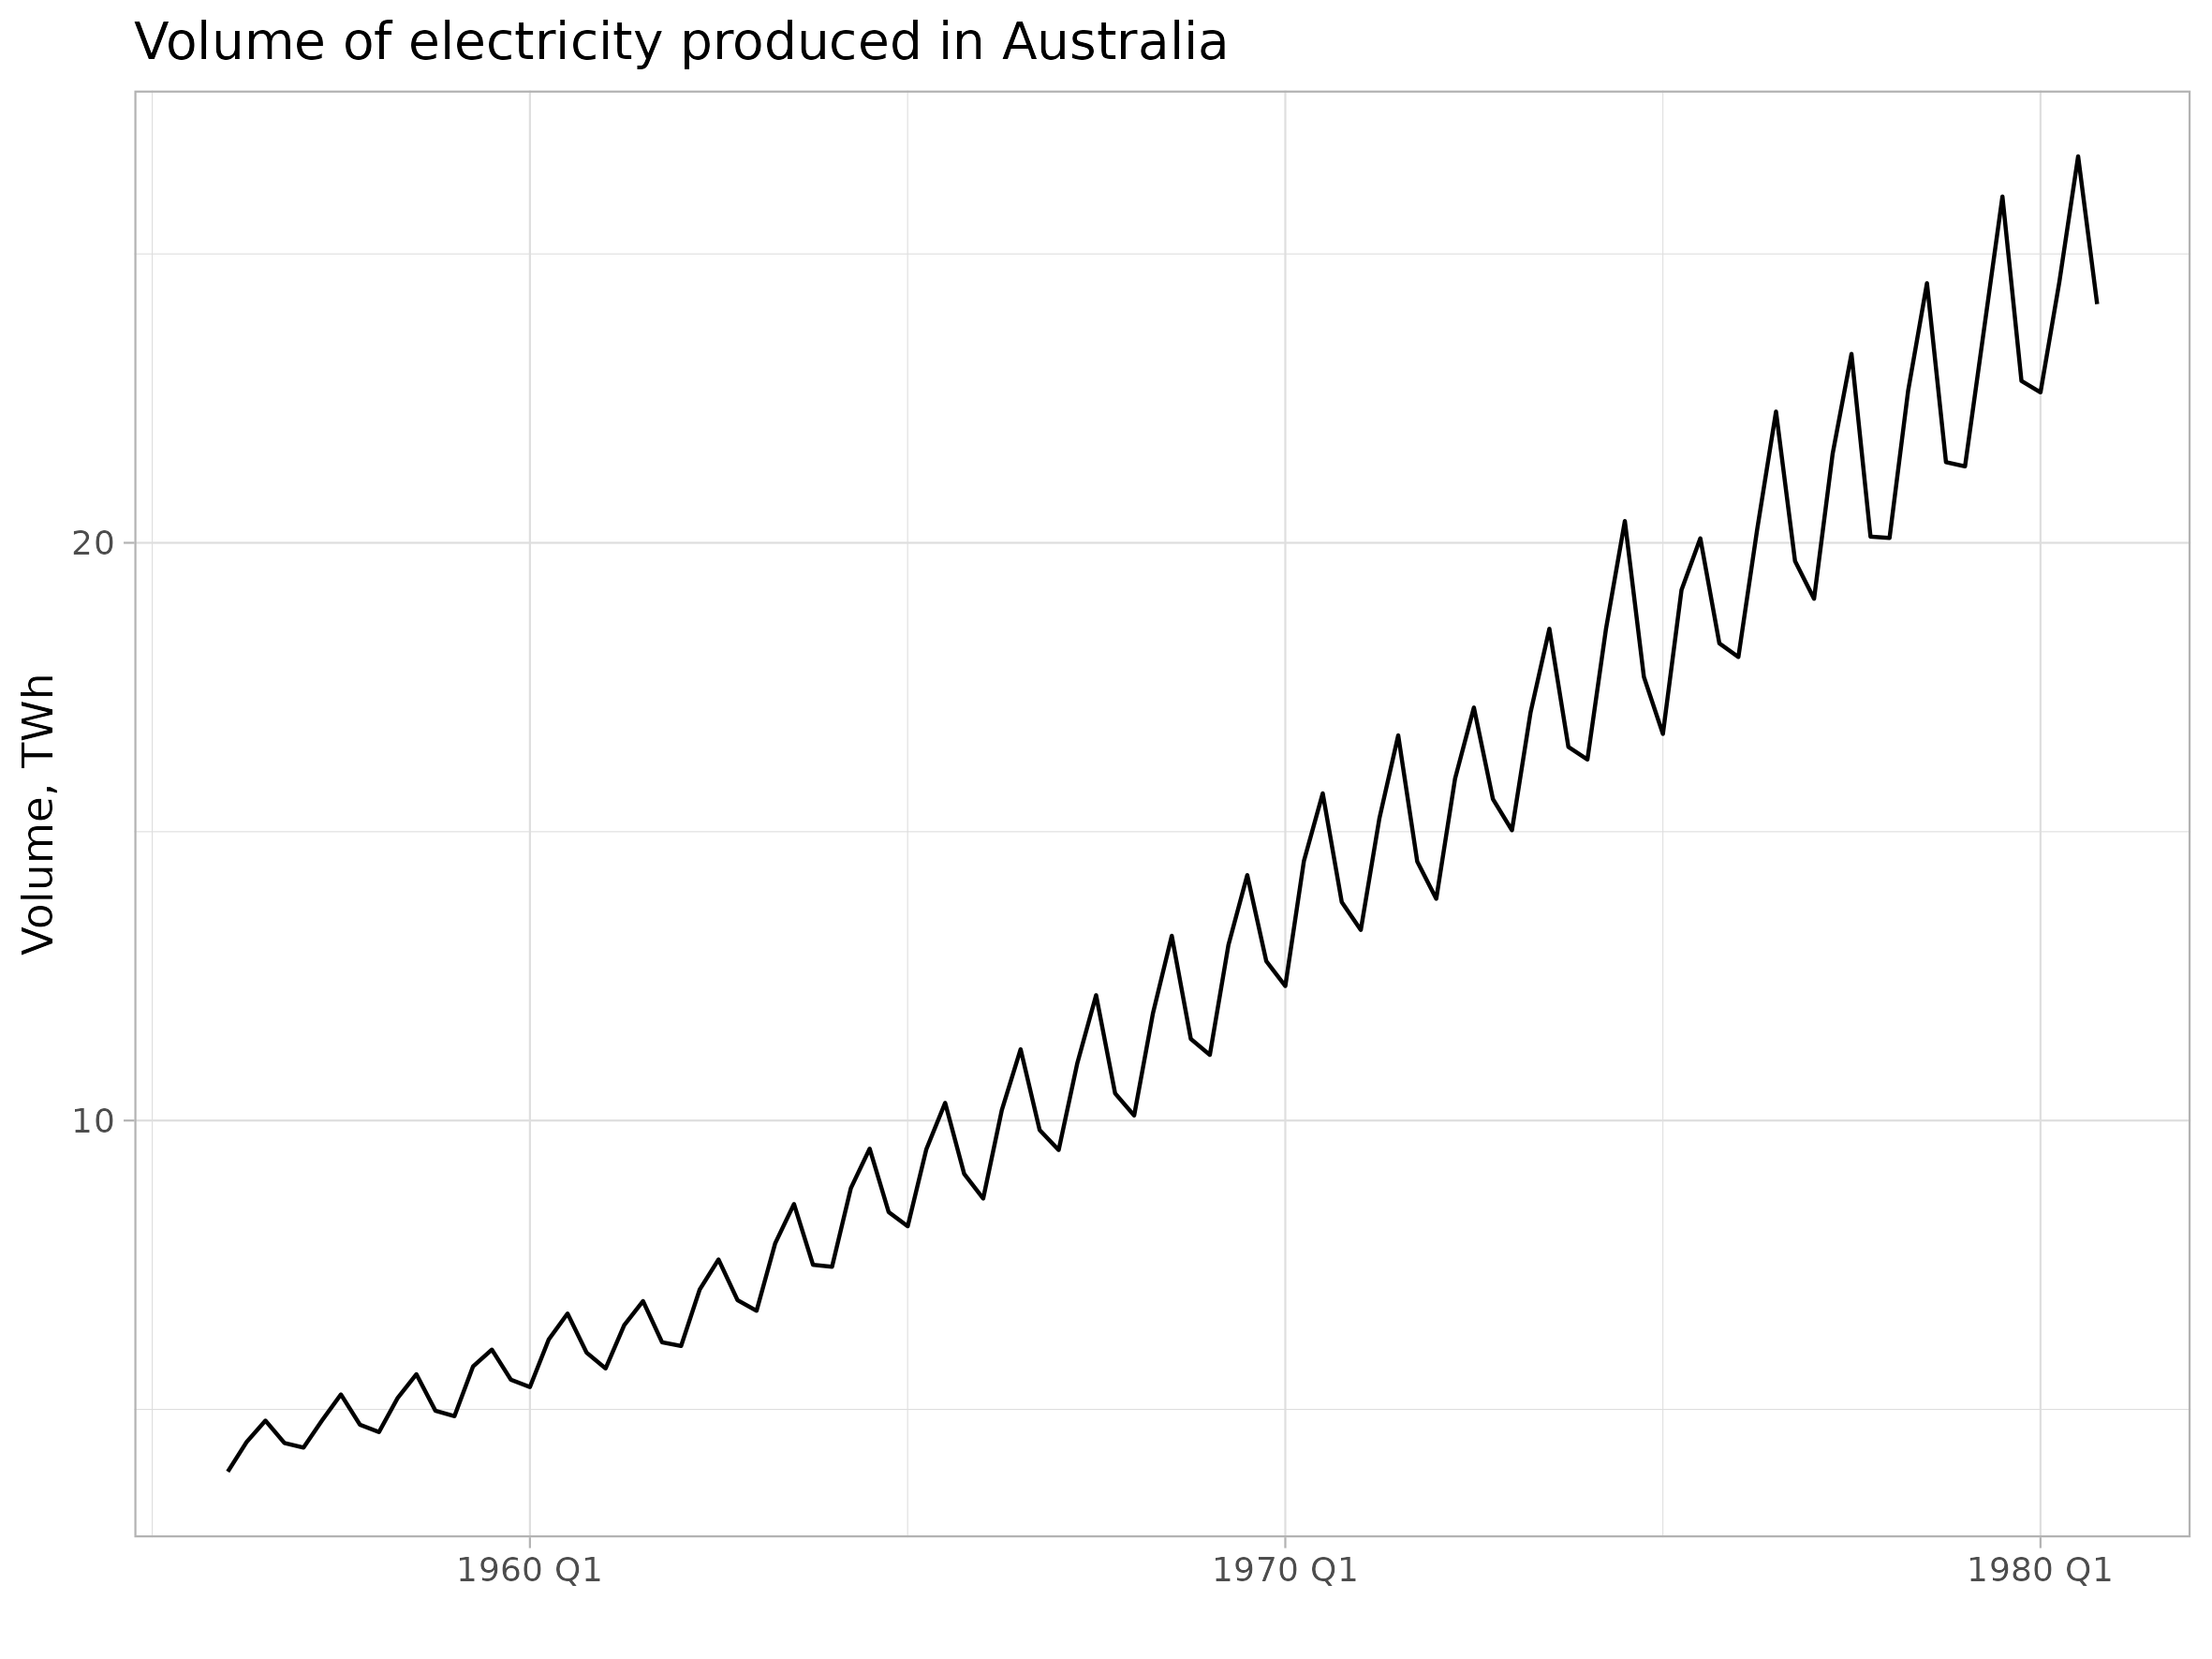
\includegraphics[width=\textwidth]{pictures/om_ts_03-033.png}
	
\end{frame}


\begin{frame}
	\frametitle{Various oscillation amplitude}
	
	Possible \alert{solutions}:
	\begin{itemize}[<+->]
		\item Switch to logarithms, $y_t \to \ln y_t$
		\item Box-Cox transformation, $y_t \to bc(y_t, \lambda)$
		\item Multiplicative components
	\end{itemize}
	
\end{frame}



\begin{frame}
	\frametitle{ETS(MNM): equations}
	
	ETS(MNM) for monthly data:
	
	\[
	\begin{cases}
		y_t = \ell_{t-1} \cdot s_{t-12} \cdot (1 + u_t); \\
		\ell_t = \ell_{t-1}\cdot (1 + \alpha u_t), \text{ starts at } \ell_0; \\
		s_t = s_{t-12}\cdot (1 + \gamma u_t), \text{ starts at } s_0, \ldots, s_{-11}; \\
		u_t \sim \dN(0;\sigma^2) \text{ and are independent} \\
	\end{cases}
	\]
	
	\pause
	ETS(ANA):
	\[
	\begin{cases}
		y_t = \ell_{t-1} + s_{t-12} + u_t; \\
		\ell_t = \ell_{t-1} + \alpha u_t, \text{ starts at } \ell_0; \\
		s_t = s_{t-12} + \gamma u_t, \text{ starts at } s_0, \ldots, s_{-11}; \\
	\end{cases}
	\]
	
\end{frame}





\begin{frame}
	\frametitle{Units}
	
	Series $y_t$, $\ell_t$ — \alert{initial} units.
	
	\pause
		
	The $s_t$ series is measured relative to one, for example, $s_t = 0.9$ — 10\% below the trend.
	
	The $u_t$ series is measured relative to zero, for example, $u_t = -0.1$ — a 10\% drop.
	
\end{frame}



\begin{frame}
	\frametitle{ETS(MNM): Forecasting}
	
	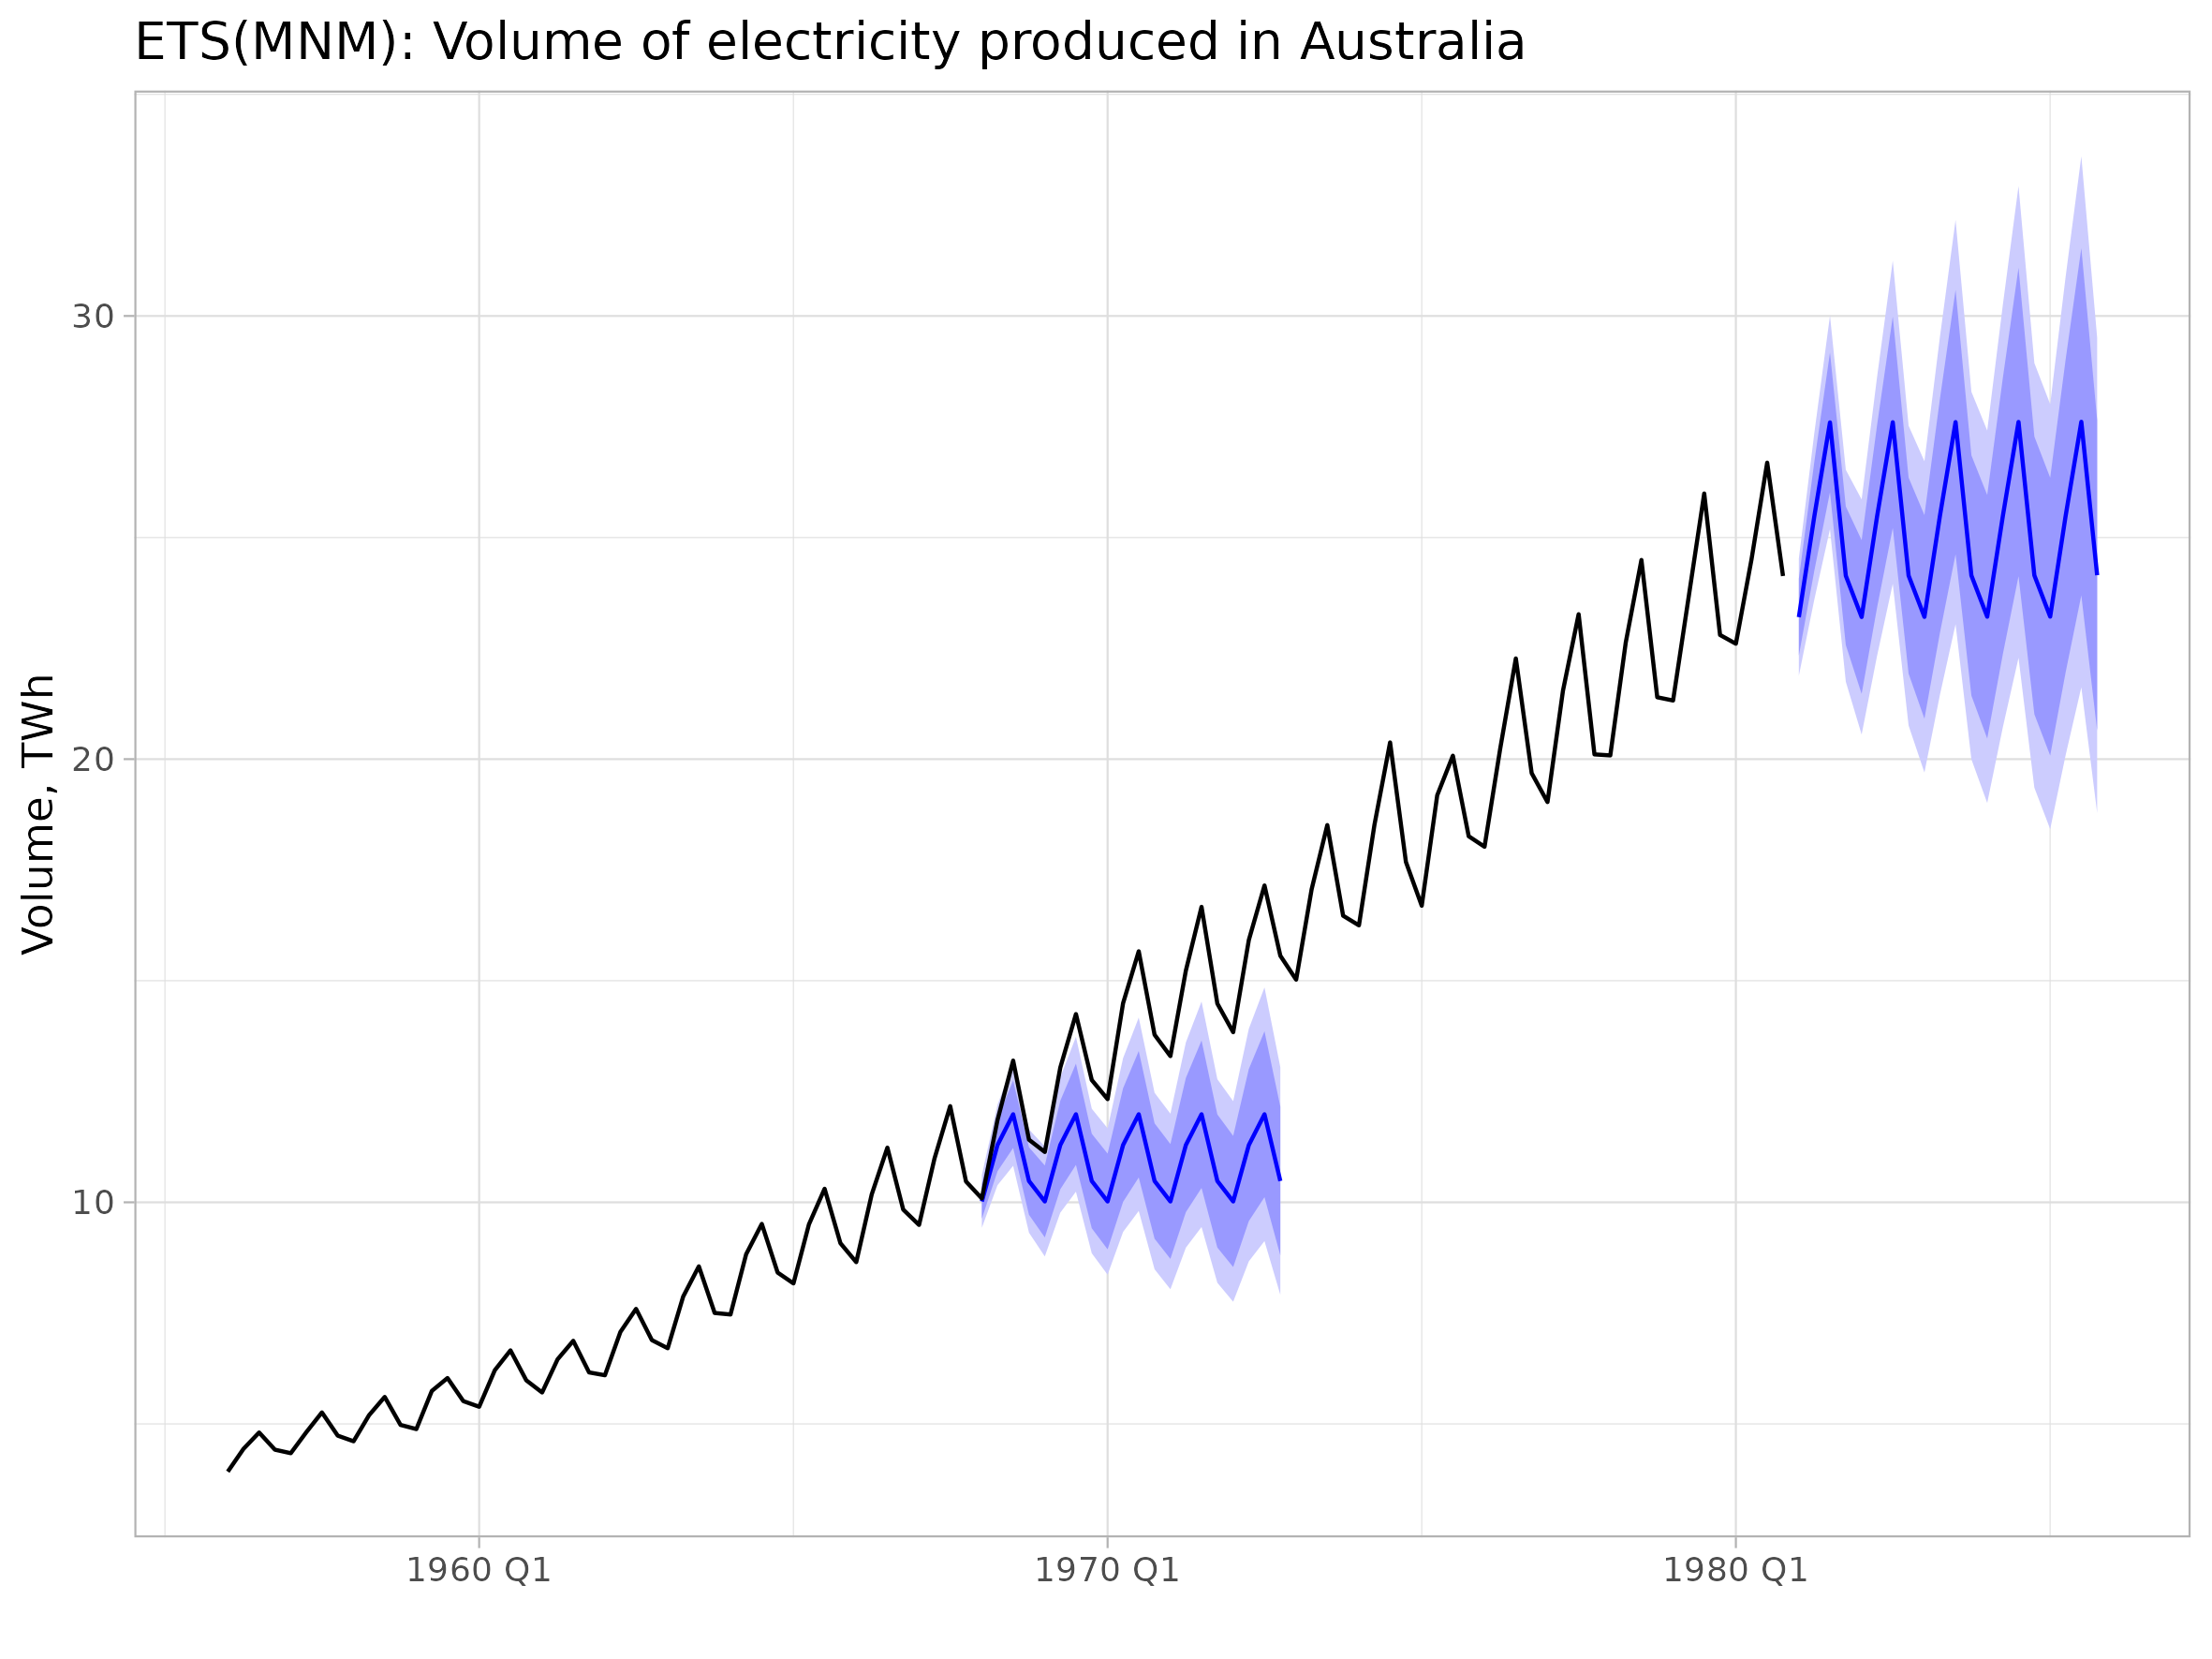
\includegraphics[width=\textwidth]{pictures/om_ts_03-047.png}
	
	
\end{frame}


\begin{frame}{Which option to choose?}
	
	\alert{Different amplitude} of fluctuations: indication of multiplicative models.
	
	\pause
	
	Automatic selection based on the \alert{AIC} criterion works.
	
	\pause
	
	
	You can get the ETS(AAdA) model \alert{with seasonality}.
	
	\pause
	
	Some of the multiplicative models can be \alert{numerically unstable}
	or \alert{not implemented} in the software.
	
\end{frame}



\begin{frame}{ETS Model: Summary}
	
	\begin{itemize}[<+->]
		\item The slope of the trend  and seasonality may change
		\item Automatic decomposition into components
		\item Multiplicative models take into account \alert{changing} oscillation amplitudes
		\item A lot of possible \alert{combinations}
	\end{itemize}
\end{frame}






% !TEX root = ../om_ts_01.tex

\begin{frame} % frame name
	
	\videotitle{Theta method}
	
\end{frame}


\begin{frame}{Theta method: Plan}
	\begin{itemize}[<+->]
		\item An unexpected leader
		\item Author's version
		\item Special case of ETS
	\end{itemize}
\end{frame}


\begin{frame}
	\frametitle{Theta method}
	
	Appeared in 2000 and became a sensation at the \alert{competition M3} for predicting series.
	
	\pause
	
	Works for \alert{non-seasonal} series.
	
	\pause
	
	Initially suggested \alert{without a statistical model}.
	
\end{frame}


\begin{frame}
	\frametitle{Author's version}
	
	\begin{enumerate}[<+->]
		\item Decompose the series into two \alert{theta lines} ($\theta=0$, $\theta = 2$) 
		\item Predict zero-line using linear regression 
		\item Predict the second line using ETS(ANN)
		\item Average the forecasts
	\end{enumerate}
	
	\pause
	You can pre-delete seasonality and add it back in the end
	
\end{frame}

\begin{frame}
	\frametitle{What is a theta line?}
	
	Zero theta line — \alert{regression} on time:
	
	\[
	\hat y_t = \hat \beta_1 + \hat \beta_2 t
	\]
	\pause
	
	Theta line for arbitrary theta:
	\[
	\Delta^2 y^{new}_t = \theta \Delta^2 y_t
	\]
	
\end{frame}


\begin{frame}{Intuition}
	
	\begin{itemize}[<+->]
		\item The zero theta line catches the long-term trend of the series
		\item Theta line ($\theta=2$) catches the short-term trend:
		
		\alert{acceleration} of theta line is $\theta$ times stronger
		than  of the initial series
		
		
		\item Averaging reduces the variance of predictions
	\end{itemize}
\end{frame}



\begin{frame}
	\frametitle{How is the theta line selected?}
	
	We take $\theta = 2$:
	\[
	\Delta^2 y^{new}_t = 2 \Delta^2 y_t
	\]
	\pause
	Or
	\[
	y^{new}_t - 2 y^{new}_{t-1} + y^{new}_{t-2} = 2(y_t - 2 y_{t-1} + y_{t-2} )
	\]
	
	\pause
	The new series $y^{new}_t$ is completely determined by $y_1^{new}$, $y_{2}^{new}$
	
	\pause
	We solve the optimization problem:
	\[
	\sum_{t=1}^T (y_t - y_t^{new})^2 \to \min
	\]
\end{frame}


\begin{frame}
	\frametitle{Statistical Model}
	
	Formal model appeared in 2003:
	
	\[
	\begin{cases}
		y_t = \ell_t + b + u_t; \\
		\ell_t = \ell_{t-1} + b + \alpha u_t; \\
		\ell_1 = y_1 \\
	\end{cases}
	\]
	
	\pause
	Or:
	\[
	\Delta y_t = b + (\alpha - 1) u_{t-1} + u_t
	\]
\end{frame}

\begin{frame}
	\frametitle{Theta method — ETS variant}
	
	A special case of a more general model — ETS(AAN):
	\[
	\begin{cases}
		y_t = \ell_{t-1} + b_{t-1} + u_t; \\
		\ell_t = \ell_{t-1} + b_{t-1} + \alpha u_t, \text{ starts at } \ell_1; \\
		b_t = b_{t-1} + \beta u_t, \text{ starts at } b_0; \\
		u_t \sim \dN(0;\sigma^2) \text{ and are independent.} \\
	\end{cases}
	\]
	\pause
	Remove the trend stochasticity setting $\beta = 0$.
	
	\pause
	\alert{Nuances} of initialization are possible.
\end{frame}




\begin{frame}{Theta method: Summary}
	
	\begin{itemize}[<+->]
		\item Works well for \alert{non-seasonal} data
		\item A special \alert{variation} of the ETS model
	\end{itemize}
\end{frame} 

\end{document}
